\chapter{A Binary Frailty model with a focus on Breast Cancer development}
\markboth{\textsc{A Binary Frailty model with a focus on Breast Cancer development}}{\textsc{A Binary Frailty model with a focus on Breast Cancer development}}\label{chapter:2}

% \author[1]{\fnm{Maria Veronica} \sur{Vinattieri}}\email{maria.vinattieri@phd.unibocconi.it}

% \author[2]{\fnm{Marco} \sur{Bonetti}}\email{marco.bonetti@unibocconi.it}
% % \equalcont{These authors contributed equally to this work.}

% \author[3]{\fnm{Kamila} \sur{Czene}}\email{kamila.czene@ki.se}
% % \equalcont{These authors contributed equally to this work.}

% \affil[1]{\orgdiv{Department of Decision Sciences}, \orgname{Bocconi University}, \orgaddress{\city{Milan}, \postcode{20136}, \state{Italy}}}

% \affil[2]{\orgdiv{Carlo F. Dondena Research Center, Bocconi Institute of Data Science and Analytics, Department of Social and Political Sciences}, \orgname{Bocconi University}, \orgaddress{\city{Milan}, \postcode{20136}, \state{Italy}}}

% \affil[3]{\orgdiv{Department of Medical Epidemiology and Biostatistics}, \orgname{Karolinska Institutet}, \orgaddress{\city{Solna}, \postcode{171 77}, \country{Sweden}}}

\begin{abstract}
We are interested on a specific aspect of survival modeling, namely the investigation of family-specific risk with a particular emphasis on the genetic component present from birth, as opposed to the environmental component. We assume that the true genetic family risk is latent and remains constant from birth. Our goal is to estimate this true family risk, as assessing the risk is crucial in improving individual survival rates by tailoring screening and prevention strategies to each individual's risk level. To achieve this goal, we employ a frailty model on the time to breast cancer onset, using a binary risk classification to divide families into low and high-risk groups. We compare this model to one that uses a strong risk factor, the family history indicator, to replace the latent risk indicator. While the family history indicator solves the issue of latency, it is a weaker indicator of the complete detailed breast cancer family history.
\textbf{keywords}: frailty models, family history of breast cancer, survival analysis
\end{abstract}

\section{Introduction}\label{sec1}
The objective of risk prediction models for breast cancer (BC) is to identify families with the highest risk of developing BC and provide them with targeted and more intensive screening and prevention approaches. These models have been extensively developed, and numerous risk factors have been incorporated to enhance their predictive power. Among the most potent risk factors for BC development is the family history indicator. Other risk factors may have a genetic nature, such as BRCA1, BRCA2, TP53, and SNPs, or a clinical and demographic nature, such as mammography density (MD) and BMI, respectively. 

Remarkable contributions to the breast cancer risk modeling field include the Gail model (refer to \cite{gail1989projecting}), which employs logistic regression to integrate risk factors, such as the number of first-degree relatives with breast cancer, and subsequently computes the long-term probability of developing breast cancer. The Tyrer and Cuzick (TC) model (refer to \cite{tyrer2004breast}) integrates personal risk factors and complete genetic analysis (involving BRCA1 and BRCA2) to model the risk of developing breast cancer by combining the genetic and familial components. The Rosner and Colditz model (refer to \cite{rosner2008risk}) is based on a log model for incidence that is affected by reproductive risk factors, including age at menarche, age at menopause, and age at childbirth. These models have been implemented in various studies, such as those described in \cite{darabi2012breast} and \cite{evans1996fictitious}.

Our objective is to develop a risk prediction model for breast cancer (BC) that considers the familial nature of the risk, which is assumed to be latent and unchanged from birth. We allow for this latent risk, also known as frailty, to be discrete and comprise two risk levels (low and high), which we denote as 0 and 1, respectively. We propose to utilize family information in a multivariate setting to more appropriately study this phenomenon. Specifically, we combine frailty theory with multivariate survival theory to develop a Cure rate Multivariate Shared Frailty model, which accommodates binary latent risk. In this model, families are treated as clusters, and individuals within a family share the same risk or frailty. Our ultimate objective is to demonstrate that this multivariate approach outperforms summary-based methods for incorporating family information  - as usually is easier and used in the literature - and it increases accuracy in risk classification. To provide a comprehensive assessment, we also implement a Cure rate Univariate Frailty model to determine the significant loss of information incurred when subjects are viewed as not part of a family sharing the risk of BC development. 

Alternatively, we compare our models to a cure rate model with the first-degree family history of breast cancer as baseline covariate. Here, family history is defined as the collection of the breast cancer experiences within a family and is represented as a binary variable that takes a value of one when at least one family member has or had breast cancer onset at the time of analysis, and zero if none did. While family history is a useful indicator of breast cancer risk, it is considered weak since it only provides a summary of the clinical history experienced by a family. For comprehensive and complex data, family history may not fully capture the familial aggregation of breast cancer development.

% One straightforward and classical choice could be working with the family history, the collection of breast cancer experiences in a family, as a time-varying covariate in a well-known model. This model specification cannot really capture the complexity that the problem is requiring. Due to this fact, we aim to compare model with the family history indicator as covariate to a Multivariate Shared Frailty model (and a derived Univariate Frailty model) to prove that performances from the first model are not even comparable to the Multivariate Frailty model performances. Notice that we also compare the Univariate frailty model to assess the crucial role that familiar information has when dealing with this problem. 

% For the Observed family history model we just replace the latent and unchanged from birth risk component $R$ with the known family history indicator. While, on the contrary, the Univariate and Multivariate model involves the unknown $R$. We allow this quantity to be discrete with two risk levels (0/1 for low/high risk of breast cancer development). Families are considered as clusters within which individuals share the same risk or frailty, where the name ``shared'' comes from.

% Our goal is to capture the complex structure that this type of data requires, but at the same time simplify the problem as much as possible to make also interpretability of results a strength point of this work. 

We introduce the methods in Section \ref{sec1}. In Section \ref{sec2} we explore the models on simulated data and we close with some discussion in Section \ref{sec6}. 

\section{Background and Model specification}\label{sec2}
% The Univariate Frailty model \cite{duchateau2008frailty} allows the hazard function to have a particular form including the frailty quantity $R$ which captures the unobserved heterogeneity among subjects. The form is given by: \[
% \lambda(t\mid R) = \lambda_0(t)R.
% \] A similar model is presented by the BOADICEA Research group. They define a multiplicative exponential hazard function that depends on a frailty component. This component, that explains the cancer family aggregation, is completely genetic and the form is given by \[
% \lambda(t\mid G = g) = \lambda_0(t)exp(\beta(g)),
% \] where $G$ is the frailty genetic quantity. The difference with out specification is that they allow $G$ to be continuous and with a genetic nature. While on the other hand we assume the risk $R$ to have not only a genetic nature, but always the explanation of the family aggregation of breast cancer. Second of all, we allow $R$ to be discrete with two ordered risk level (low risk and high risk). At the end of the day, the hazard specification is given by: \[
% \lambda_0(t) = \lambda_0(t) \qquad \lambda_1(t\mid R) = \lambda_0(t)\alpha(R) = \lambda_0(t)\alpha.
% \] where ``0'' refers to the low-risk hazard, and ``1'' refers to the high-risk hazard, and with $\alpha$ the frailty parameter. This last parameter $\alpha$ should be greater than one in order to keep valid that $\lambda_1$ is the hazard function of the highest risk group. Otherwise the order is flipped. 

% We rely on the Multivariate Survival model theory to involve all the survival information from the same family. For a family of two people the survival function is given by \cite{hougaard2012analysis, rodriguez2010multivariate}: \[
% S_{12}(t_1,t_2\mid \alpha) = S_1(t_1\mid \alpha)S_2(t_2\mid \alpha),
% \] due to the assumption of \textbf{Conditional Independence} in the frailty model. This result can be readily generalized to more than two members of a family, because of the multiplicative form of the survival function. Moreover, we can explicit the Lehmann structure of the survival function, starting from $\lambda(t) = \lambda_0(t)\alpha$, in the following way: \[
% S(t) = [S_0(t)]^\alpha \qquad S_{12}(t_1,t_2\mid \alpha) = [S_0(t_1)S_0(t_2)]^\alpha,
% \] where the generalized formula is then given by: \[
% S_{\text{family}}(\underline{t}\mid R) = \left[\prod_{j=1}^{n_i}S_0(t_j)\right]^\alpha
% \] where $\underline{t} = (t_1, \dots, t_{n_i})^T$, with $n_i$ the sample size of the $i$th family. 

% Hence, we introduce the frailty models in the multivariate setting \cite{hougaard2012analysis}. The name ``multivariate'' holds for referring to many outcomes (time-to-event), not just to many explanatory variables \cite{rodriguez2010multivariate}.Taking into account the problem of family history in breast cancer, if two women belong to the same family, their time-to-event are dependent. The assumption of conditional independence holds in this setting, conditional to the family. Let $T_1 = t_1$, and $T_2 = t_2$, be the time-to-events of two women in a family, and $r$ the frailty value, then the assumption of conditional independence allows the joint survival function to be \begin{align*}
%     S_{12}(t_1,t_2\mid r) \overset{T_1\perp T_2\mid R}{=} S_1(t_1\mid r)S_2(t_2\mid r).
% \end{align*} This case can be readily generalized to more than two survival times. 
The Univariate Frailty model \cite{duchateau2008frailty} on the time to event $T = t$ allows the hazard function $\lambda(t\mid r)$ to have a particular form including the frailty quantity $R$ which captures the unobserved heterogeneity among subjects. Tha hazard is given by 
\[
\lambda(t\mid R = r) = \alpha(r)\lambda_0(t),
\] 
where $\lambda_0(t)$ is the baseline hazard function that can assume a a parametric with parameter collection $\underline{\theta}$ or a semi-parametric form; and $\alpha(r)$ is a general function of the risk but we will use the linear form $\lambda(t\mid r) = r\lambda_0(t)$. The model can be extended to the inclusion of subject-specific covariates. In this case the frailty quantity explains the unobserved heterogeneity that the covariates are not able to capture. The hazard is given by: \[
\lambda_j(t\mid R = r) =r\lambda_0(t;x_j),
\] 
where $x_j$ are the covariates of the $j$th subject. The shared frailty hazard function allows to define the frailty as a family-specific quantity. Thus, this specification is used with clustered data, as it is our case, where the shared frailty hazard is given by:
\[
\lambda_{ij}(t\mid R = r_i) = r_i\lambda_0(t;x_{ij}),
\] 
with $x_{ij}$ the $i$th subject-specific covariates in the $j$th family. 

In the binary case, the latent quantity can be represented as $r = (r_0, r_1)$, where typically $r_0 = 1$. This assumption allows the hazard and survival functions of group ``0'' to coincide with the baseline functions, while $r_1 = r>1$ ensures coherence with the assumption of a highest-risk group in the population and thus with the assumption of proportional hazard. Therefore, we obtain: \begin{align*}
    &\lambda_0(t) = \lambda_0(t;x_{ij}), S_0(t) = S_0(t;x_{ij}), \\
    &\lambda_1(t) =  r \lambda_0(t;x_{ij}), S_1(t) = [S_0(t;x_{ij}) ]^r.
\end{align*}

Thus, we introduce frailty models in a multivariate setting \cite{hougaard2012analysis}. The term ``multivariate'' refers to the inclusion of multiple outcomes, i.e., time-to-event, within the same family \cite{rodriguez2010multivariate}. We handle multiple time-to-event data by leveraging the assumption of conditional independence. For instance, consider the case where two women belong to the same family, resulting in dependent time-to-events. However, assuming conditional independence given the family, let $T_1 = t_1$ and $T_2 = t_2$ be the time-to-events of the two women in the family, and let $r$ denote the frailty value, we can express the joint survival function as follows: \begin{align*}
    S_{12}(t_1,t_2\mid R = r) \overset{T_1\perp T_2\mid R}{=} S_1(t_1\mid R = r)S_2(t_2\mid R = r).
\end{align*} Hence, if $R = 1$, we have \[
    S_{12}(t_1,t_2) = S_0(t_1)S_0(t_2),
\] while, if $R = r>1$, we have \[
    S_{12}(t_1,t_2) = S_1(t_1)S_1(t_2) = [S_0(t_1)S_0(t_2)]^r.
\] It is important to note that this case can be easily extended to more than two survival times per cluster sharing the same risk $R$. The marginal survival function for $n_i$ subjects per family is given by: \[
S_{1\dots n_i}(t_1,\dots,t_{n_i}) = h\prod_{j=1}^{n_i}S_0(t_j) + (1-h)\prod_{j=1}^{n_i}\left[S_0(t_j)\right]^r
\] where $S_0(t_j) = p_0 + (1-p_0)\widetilde{S}_0(t_j)$ and $h$ the probability of belonging to a low-risk family in population.

Given the nature of the phenomenon, not all women will experience breast cancer, regardless of how long they live, as is the case with death. Therefore, we use the cure rate survival function \cite{mota2022new}, which can be considered as a mixture of a proper survival function, which models the fraction of individuals who will experience the event, and a degenerate distribution, which models the fraction of individuals who will not experience the event. The mixture survival function is given by: \[
S_0(t) = p_0 + (1-p_0)\widetilde{S}_0(t)
\] with $\widetilde{S}_0(t)$ the proper survival function, and $p_0$ the probability of being cured. Recall the Lehmann structure on the survival function characterizing the risk group $S_r(t) = [S_0(t)]^{\alpha(r)}$, such that in the end we have \begin{align*}
    &S_0(t) = p_0 + (1-p_0)\widetilde{S}_0(t) &S_1(t) = [p_0 + (1-p_0)\widetilde{S}_0(t)]^r
\end{align*} For a fixed $r$, also the high-risk survival function $S_1(t)$ defines a cure rate model. % We identify the latent risk as a parameter $\alpha$ to be estimated. The proportional hazard (PH) structure allows the hazard function in a risk group to be written in function of the baseline hazard $\lambda_0(t)$, such that $\lambda_r(t) = \alpha(r) \lambda_0(t)$ (in particular $\lambda_0(t)$, and $\lambda_1(t) = \alpha \lambda_0(t)$), where $\lambda_0(t)$ is distributed according to a parametric distribution identified by the parameter collection $\underline{\theta}$, or a semiparametric distribution. Hence, it follows that the survival function is identified by a Lehmann structure, such that $S_r(t)=[S_0(t)]^{\alpha(r)}$. We thus have $S_0(t)$, and $S_1(t) = [S_0(t)]^{\alpha}$. Recall that the baseline survival function is defined by the more general Lehmann cure-rate family obtained by applying the Lehmann power transformation to a cure-rate survival function $S_r(t) = \left[p_0 + (1-p_0) \widetilde{S}(t) \right]^{\alpha(r)}$, with $\widetilde{S}(t)$ a proper survival function, so that we have $S_0(t) = p_0 + (1-p_0) \widetilde{S}(t)$, and $S_1(t) = [p_0 + (1-p_0) \widetilde{S}(t)]^\alpha$. For a fixed value $\alpha$, the aforementioned model is such that the survival function $S_1(t)$ also defines a cure-rate model. 
It is easy to check that $\lim_{t \rightarrow \infty} S_{1}(t) = p_0^r = p_1$, and that $S_1(t)$ can be written as
\[
S_1(t) = p_1 + \left( 1-p_1\right) \widetilde{S}_1(t),
\]
with conditional (proper) survival function for the cases equal to:
\[
\widetilde{S}_1(t) = \dfrac{\left[p_0 + (1-p_0) \widetilde{S}_0(t) \right] ^r - p_0^{r}}{1-p_0^{r}},
\]
and conditional density function: 
\[
\widetilde{f}_1(t) = - \dfrac{d}{d t} \widetilde{S}_1(t) = \dfrac{1-p_0}{1-p_0^{r}} r \left[p_0 + (1-p_0) \widetilde{S}_0(t) \right]^{\left(r -1 \right)} \widetilde{f}_0(t).   
\]
Since the cure rate survival function is not proper, the density function associated with the cure rate model is also not proper. For simplicity, we have not included the term related to the risk thus far. To incorporate the risk group, we can rewrite the survival function $S_r(t) = [S_0(t)]^r$ as a function that depends on the risk group. Therefore, the generalized model is expressed as:
\begin{align*}
    % S(T=t\mid R=r) = 
    S_r(t) = S(T=t\mid R=r) = [S_0(t)]^r, \ r \in \{r_0,r_1\}.
\end{align*} 
Note that if $T\sim S_0(t)$, then $P(T=+\infty)=p>0$, and a proper density function $f_T(t)$ does not exist. 

\begin{lem}
If $S(t)$ follows a cure rate structure, then it does not admit a density with respect to the Lebesgue measure. 
\begin{proof}
Note that we have \begin{align}
    \label{formula:lemma_1}
    \lim_{t\to\infty}S(t)= \lim_{t\to\infty}(p+(1-p)\widetilde{S}(t))=p>0
\end{align}
Suppose that a density function $f(t)$ exists so that $S(t)=\lim_{t\to\infty}\int_t^\infty f(u)\text{d}u$ and $\int_0^\infty f(u)\text{d}u=1$. Then, we will prove that \begin{align*}
    &\lim_{t\to\infty}{\int_{t}^\infty f(u)\text{d}u}=0 \\
    &\lim_{t\to\infty}{\int_{t}^\infty f(u)\text{d}u} = \lim_{t\to\infty}{\int_{0}^\infty \mathbbm{1}(s\ge t)f(s)\text{d}s} 
\end{align*}
We apply the dominated convergence \cite{weir1973lebesgue}: \begin{align*}
    &\text{since }\mathbbm{1}(s\ge t)f(s) \le f(s) \ \forall s\ge 0 \text{ and } \int_0^\infty f(s)\text{d}s=1; \\
    &\Rightarrow \int_0^\infty \mathbbm{1}(s\ge t)f(s) \le \int_0^\infty f(s)\text{d}s = 1. \\
    &\text{Then, } \lim_{t\to\infty}S(t) = \lim_{t\to\infty}{\int_{t}^\infty f(s)\text{d}s} = \lim_{t\to\infty}{\int_{0}^\infty \mathbbm{1}(s\ge t)f(s)\text{d}s} \\
    &\qquad\qquad\qquad\quad\overset{\overset{DCI}{\downarrow}}{=} \int_{0}^\infty\lim_{t\to\infty} (\mathbbm{1}(s\ge t)f(s))\text{d}s=0,
\end{align*}
\end{proof}
\end{lem}

which contradicts formula \ref{formula:lemma_1}. Thus, as expected, a proper density function associated with a cure rate survival function does not exist. Indeed, the density function conditionally to the uncured rate proportion $f(t) = (1-p)\widetilde{f}(t)$ is improper, as the cure rate marginal density function.

Once the baseline function of the two risk groups are defined we can move to the building of the likelihood. 

% We want to prove that a Multivariate Survival model, with the information on the family risk $R$ not available, has better performance than the model where we replace the unknown frailty with a known parameter. Additionally, we will prove the crucial function that families have in assessing the role of the frailty, so we also show the Univariate version of the former model said.

% The vanilla version of a multivariate shared frailty survival model, since it only admits the existence of two risk groups, with conditionally independent survival times within each family. The extension to k-groups of infinite groups is straightforward and shown afterward. 

% Parameter estimation is achieved through the (probably numerical) maximization of the likelihood. The specification of the likelihood is explained in the following lines. 

Let us consider families with three members, but it should be noted that this can be extended to families with different numbers of members. In each of the $G$ families included in our sample, we identify one woman $i$ as the main subject, and use $\{m,s_1\}$ to denote the other two family members, the mother and the first sister, respectively. The observed data can be expressed as: $\underline{\textbf{Z}}=\left(\underline{\textbf{Z}}_1,\dots,\underline{\mathbf{Z}}_G\right)^T$, where $\underline{\textbf{Z}}_i=(\underline{\textbf{z}}_i, \underline{\textbf{zs}}_{1i}, \underline{\textbf{zm}}_i)^T$. 
For the generic subject $j$, $\underline{\textbf{z}}_{j}=(z_{j}=\text{min}(t_{j}, c_{j}),\delta_{j})^T$, $\delta_{j}=\mathbb{I}(t_{j} \le c_{j})$ following the usual notation that has $t_j$ indicate the survival time, where in our case is the age in years at breast cancer onset, and $c_j$ indicate the independent censoring time, both measured from the same origin. The notation for the other family members is obtained by having $z, \ t, \ c, \ b$ be followed by $s_1$ and $m$ as shown above. The distinction between mother and sister is not strictly needed here, it will make the extension to a more complex model easier.

We define the multivariate likelihood function as $L(\underline{\zeta};\underline{\mathbf{Z}})=\prod_{i=1}^G f_Z(\underline{\textbf{Z}}_i;\underline{\zeta})$, where $\underline{\zeta}=\{r, h, p_0, \underline{\theta}\}^T$ represents the parameter collection. Here, $r$ is the target parameter for inference: the risk difference between the low-risk and the high-risk group of developing breast cancer in this special case of two risk groups, involved in the hazard PH structure: $\lambda_1(t) = r\lambda_0(t)$. Then we have $p_0$ that represents the proportion of cured fraction of individuals in the population, $P(R=1) = h$ is the proportion of high risk families in the population, and $\underline{\theta}$ represents the collection of baseline survival parameters. The survival and density functions follow a Lehmann structure for the high risk group, as: \begin{align*}
    &S_1(t) = \left[ p_0 + (1-p_0) \widetilde{S}_0(t) \right]^{r} = p_0^r + (1-p_0^r) \widetilde{S}_1(t), \\
    &\widetilde{S}_1(t) = \dfrac{\left[ p_0 + (1-p_0) \widetilde{S}_0(t) \right] ^{r} - p_0^{r}}{1-p_0^{r}}, \\
    &f_1(t) = (1-p_0^r)\widetilde{f}_1(t), \\
    &\widetilde{f}_1(t) = \dfrac{r ( 1 - p_0)}{1- p_0^r}  \left[ p_0 + (1-p_0 ) \widetilde{S}_0(t) \right]^{r -1}  \widetilde{f}_0 (t).
\end{align*} Hence, we can obtain the likelihood function by: \begin{align}
    \label{share_frailty_model}
    L(\underline{\zeta};\underline{\mathbf{Z}})=\prod_{i=1}^G f_Z(\underline{\textbf{Z}}_i; \underline{\zeta}) = \prod_{i=1}^G & [P(R_i=0) f_Z(\underline{\textbf{Z}}_i \mid R_i=0;\underline{\zeta}) \\
    & +P(R_i=1)f_Z(\underline{\textbf{Z}}_i \mid R_i=1;\underline{\zeta})]. \nonumber
\end{align} 
To fix ideas, the family risk $R$ is treated as a latent variable and integrated out in the likelihood function. However, if $R$ was known for each family, then there would be no need to integrate over the distribution of $R$ in the likelihood. This is in contrast to models that use an observable indicator in place of the true risk indicator.
% A generalization of how to build the likelihood function in the censoring case is explained in Appendix \ref{appendix:b}.

For ease of notation we drop writing the baseline survival parameter collection $\underline{\theta}$ below. The first component is obtained, under the assumption of conditional independence of the survival times within each family, as:
\begin{align*}
    &f_Z(\underline{\textbf{z}}_i\mid R_i=0) =  \left[f_T(z_i\mid R_i=0)S_C(z_i)\right]^{\delta_i} \left[S_T(z_i\mid R_i=0)f_C(z_i)\right]^{1-\delta_i} \\
    &\qquad\qquad\qquad\propto f_T(z_i\mid R_i=0)^{\delta_i}S_T(z_i\mid R_i=0)^{1-\delta_i} \\
    &\qquad\qquad\qquad=\left[((1-p_0)\widetilde{f}_0(z_{i}))^{\delta_{i}}(p_0+(1-p_0)\widetilde{S}_0(z_i))^{(1-\delta_{i})}\right] \\
    &f_Z(\underline{\textbf{zs}}_i\mid R_i=0) = f_T(zs_i\mid R_i=0)^{\delta s_i}S_T(zs_i\mid R_i=0)^{1-\delta s_i} = \\
    &=\left[((1-p_0)\widetilde{f}_0(zs_i))^{\delta s_i}(p_0+(1-p_0)\widetilde{S}_0(zs_i))^{(1-\delta s_i)}\right] \\
    &f_Z(\underline{\textbf{zm}}_i\mid R_i=0) = f_T(zm_i\mid R_i=0)^{\delta m_i}S_T(zm_i\mid R_i=0)^{1-\delta m_i} = \\
    &=\left[((1-p_0)\widetilde{f}_0(zm_i))^{\delta m_i}(p_0+(1-p_0)\widetilde{S}_0(zm_i))^{(1-\delta m_i)}\right] \\
    &f_Z(\underline{\textbf{Z}}_i;\underline{\zeta}\mid R_i=0) \overset{\perp\mid R}{=} f_Z(\underline{\textbf{z}}_i\mid R_i=0)f_Z(\textbf{zs}_i\mid R_i=0)f_Z(\textbf{zm}_i\mid R_i=0) \\ 
    &\qquad\qquad\qquad= \left[((1-p_0)\widetilde{f}_0(z_{i}))^{\delta_{i}}(p_0+(1-p_0)\widetilde{S}_0(z_i))^{(1-\delta_{i})}\right]\cdot \\
    &\qquad\qquad\qquad\cdot\left[((1-p_0)\widetilde{f}_0(zs_i))^{\delta s_i}(p_0+(1-p_0)\widetilde{S}_0(zs_i))^{(1-\delta s_i)}\right]\cdot \\
    &\qquad\qquad\qquad\cdot\left[((1-p_0)\widetilde{f}_0(zm_i))^{\delta m_i}(p_0+(1-p_0)\widetilde{S}_0(zm_i))^{(1-\delta m_i)}\right].
\end{align*}
Similarly for the second component we have:
\begin{align*}
    &S_1(z_i) = S_T(z_i\mid R_i=1) = [S_T(z_i\mid R_i=0)]^{r} = [S_0(z_i)]^{r} \\
    &\qquad\=[p_0+(1-p_0)\widetilde{S}_0(z_i)]^{r} = p_1 + (1-p_1)\widetilde{S}_1(z_i) \\ 
    &p_1 = p^{r}\text{ and, } \widetilde{S}_1(z_i)=\dfrac{(p_0+(1-p_0)\widetilde{S}_0(z_i))^{r}-p_1}{1-p_1} \\
    &f_1(z_i) = (1-p_1)\left(\dfrac{1-p_0}{1-p_1}\right)r\widetilde{f}_0(t)\left(p_0+(1-p_0)\widetilde{S}_0(z_i)\right)^{r-1} \\
    &f_Z(\textbf{z}_i\mid R_i=1) = \left[f_T(z_i\mid R_i=1)S_C(z_i)\right]^{\delta_i} \left[S_T(z_i\mid R_i=1)f_C(z_i)\right]^{1-\delta_i} \\
    &\propto f_T(z_i\mid R_i=1)^{\delta_i}S_T(z_i\mid R_i=1)^{1-\delta_i}=f_1(z_i)^{\delta_i}S_1(z_i)^{1-\delta_i} \\
    &=\left[\dfrac{r\widetilde{f}_0(z_i)}{(1-p_0)^{-1}}\left(p_0+(1-p_0)\widetilde{S}_0(z_i)\right)^{r-1} \right]^{\delta_i}\cdot\left[p_1 + (1-p_1)\widetilde{S}_1(z_i)\right]^{1-\delta_i} \\
    % &\qquad\qquad\qquad= e^{r\delta_i}(1-p)^{\delta_i}\widetilde{f}(z_i)^{\delta_i}\left[p+(1-p)\widetilde{S}(z_i)\right]^{e^r-\delta_i} \\
    &f_Z(\textbf{zs}_i\mid R_i=1) = f_1(zs_i)^{\delta s_i}S_1(zs_i)^{1-\delta s_i} = \\ &=\left[\dfrac{r\widetilde{f}_0(zs_i)}{(1-p_0)^{-1}}\left(p_0+(1-p_0)\widetilde{S}_0(zs_i)\right)^{r-1} \right]^{\delta s_i}
    \left[p_1 + (1-p_1)\widetilde{S}_1(zs_i)\right]^{1-\delta s_i} \\
    % &f_Z(\textbf{z}_{m_i}\mid R_i=1) = f_1(zm_i)^{\delta m_i}S_1(zm_i)^{1-\delta m_i} = e^{r\delta m_i} (1-p)^{\delta m_i}\widetilde{f}(zm_i)^{\delta m_i}\left[p+(1-p)\widetilde{S}(zm_i)\right]^{e^r-\delta m_i} \\
    &f_Z(\textbf{zm}_i\mid R_i=1) = f_1(zm_i)^{\delta m_i}S_1(zm_i)^{1-\delta m_i} = \\
    &=\left[\dfrac{r\widetilde{f}_0(zm_i)}{(1-p_0)^{-1}}\left(p_0+(1-p_0)\widetilde{S}_0(zm_i)\right)^{r-1} \right]^{\delta m_i}\left[p_1 + (1-p_1)\widetilde{S}_1(zm_i)\right]^{1-\delta m_i} \\
    &f_Z(\underline{\textbf{Z}}_i;\underline{\zeta}\mid R_i=1) \overset{\perp\mid R}{=} f_Z(\textbf{z}_i\mid R_i=1)f_Z(\textbf{zs}_i\mid R_i=1)f_Z(\textbf{zm}_i\mid R_i=1)
\end{align*}
% qui
The specific mathematical calculations for the most common baseline survival distributions, i.e., the Exponential and the Weibull distributions, are presented in Appendix \ref{appendix:c} and Appendix \ref{appendix:d}, respectively.

In the case where not all familial breast cancer information is available, one may use the univariate likelihood instead of the multivariate likelihood. In this scenario only one subject per family contributes to the likelihood. As before, the goal of parameter estimation is to determine the risk difference $r$ between the low and high-risk groups, so the parameter collection is still denoted by $\underline{\zeta}=\{r, h, p_0, \underline{\theta}\}^T$. The likelihood function can be derived as follows. Note that the survival and density functions for the low and high-risk groups are given by: \begin{align*}
    % \label{unvariate_shared_frailty}
    &S_0(z_i) = p_0+(1-p_0)\widetilde{S}_0(z_i) \nonumber \\
    &f_0(z_i) = (1-p_0)\widetilde{f}_0(z_i) \nonumber \\
    &S_1(z_i) = [S_0(z_i)]^{r} = [p_0+(1-p_0)\widetilde{S}_0(z_i)]^{r} 
    = p_1 + (1-p_1)\widetilde{S}_1(z_i) \nonumber \\ 
    &f_1(z_i) = (1-p_1)\left(\dfrac{1-p_0}{1-p_1}\right)r\widetilde{f}_0(t)\left(p_0+(1-p_0)\widetilde{S}_0(z_i)\right)^{r-1}\nonumber \\
    &\text{with, }p_1 = p^{r}\text{ and, } \widetilde{S}_1(z_i)=\dfrac{(p_0+(1-p_0)\widetilde{S}_0(z_i))^{r}-p_1}{1-p_1}.\nonumber 
\end{align*} Thus, the likelihood is given by: \begin{align}
    L_u(\underline{\zeta};\underline{\mathbf{z}}) &=\prod_{i=1}^G f_Z(\underline{\textbf{z}}_i;\underline{\zeta}) = \prod_{i=1}^G[f_Z(\underline{\textbf{z}}_i\mid R_i=0;\underline{\zeta})P(R_i=0) \\
    &+f_Z(\underline{\textbf{z}}_i\mid R_i=1;\underline{\zeta})P(R_i=1)] \nonumber \\
    &= \prod_{i=1}^G\left[f_0(z_i)^{\delta_i}S_0(z_i)^{1-\delta_i}\right](1-h)+\left[f_1(z_i)^{\delta_i}S_1(z_i)^{1-\delta_i}\right] h. \nonumber
\end{align} where subscript ``u'' stays for univariate likelihood. 

Given the latent nature of the risk quantity, it may be necessary to replace it with an observable indicator. In this setting, we replace the frailty with the indicator of an observed family history of breast cancer. Specifically, we consider a subject $i$ and define $FH(u)$ as the indicator function that takes value $1$ if one or more relatives of the subject have experienced the disease by the subject age $u$. For a family with three members, we have for example $FH(u) = 1 - \mathbb{I}(bm+tm\ge b+t)\mathbb{I}(bs_1+ts_1\ge b+t)=1 - \mathbb{I}(tm\ge t+30)\mathbb{I}(ts_1\ge t)$. The general form of the survival function depending on $FH(u)$ is given by: \[
S_F(z_i) = [S_0(z_i)]^{\beta_F FH(z_i)}.
\]
Again, the baseline cure rate survival and density functions are given by 
\begin{align*}
    &S_0(z_i) = p_0+(1-p_0)\widetilde{S}_0(z_i) 
    &f_0(z_i) = (1-p_0)\widetilde{f}_0(z_i) \nonumber \\
    % &\widetilde{S}(z_i) = S(z_i \mid FH(t)=f) = [S_0(z_i)]^{{\beta_F}f}
\end{align*} Consequently, for the high-risk group we have
\begin{align*}
    &S_1(z_i) = [S_0(z_i)]^{\beta_F} =[p_0+(1-p_0)\widetilde{S}_0(z_i)]^{\beta_F} =p_1 + (1-p_1)\widetilde{S}_1(z_i) \nonumber \\ 
    &f_1(z_i) = (1-p_1)\left(\dfrac{1-p_0}{1-p_1}\right)\beta_F\widetilde{f}_1(t)\left(p_0+(1-p_0)\widetilde{S}_0(z_i)\right)^{{\beta_F}-1} \nonumber \\
    &\text{with, }p_1 = p^{{\beta_F}}\text{ and, } \widetilde{S}_1(z_i)=\dfrac{(p_0+(1-p_0)\widetilde{S}_0(z_i))^{{\beta_F}}-p_1}{1-p_1} \nonumber
\end{align*}
The parameter $\beta_F$ is the observed family history risk modifier, and it is typically used to account for the increased family risk for subjects that have a positive family history of breast cancer. In other words, $FH(t)$ is meant to estimate the latent risk group $R$ from the observed onset histories at time of the analysis $t$. Importantly, in the trivial case of two risk groups, while $R$ takes value zero or one from birth and does not change over time, $FH(t)$ is a counting process that takes value one as soon as the first onset occurs among any of the other family members. Replacing the true unknown risk group $R$ with the dummy $FH(t)$ makes us falling into a measurement error. A detailed section about measurement error is reported in Appendix \ref{appendix:e}. Moreover, a comparison of $FH$ vs. $R$ in terms of probability of agreement is run in Appendix \ref{appendix:f}.

The parameter collection is $\underline{\zeta}_{FH}=\{\beta_F, p_0, \underline{\theta}\}^T$. The univariate likelihood involving the family history indicator is given by  \begin{align}
    \label{model_FH}
    &L^*(\underline{\zeta}_{F};\underline{\mathbf{z}},\underline{FH}) = \prod_{i=1}^G f_Z(\underline{FH}, \underline{\textbf{z}}_i;\underline{\zeta}_F) \\
    &\qquad\qquad=\prod_{i=1}^Gf_Z(\underline{\textbf{z}}_i\mid FH_i=0;\underline{\zeta}_F)^{(1-FH_i)}f_Z(\underline{\textbf{z}}_i\mid FH_i=1;\underline{\zeta}_F)^{FH_i} \nonumber \\ 
    &\qquad\qquad= \prod_{i=1}^G\left[f_0(z_i)^{\delta_i}S_0(z_i)^{1-\delta_i}\right]^{(1-FH_i)}\left[f_1(z_i)^{\delta_i}S_1(z_i)^{1-\delta_i}\right]^{FH_i} \nonumber
\end{align} 
We need to fix the baseline distribution. Some common proposals are the Exponential, the Weibull, and the Gamma distribution. The parameter estimation is achieved then by maximizing the log-likelihood. A numerical method for likelihood maximization is chosen among the available ones. We chose to run a Nelder-Mead optimization. 

A note on parameter identifiability is reported in Appendix \ref{appendix:a}.

The estimated parameters can be used to generate posterior risk predictions, which are the focus of this project. The objective is to internally validate the model by accurately predicting the risk of breast cancer development for each woman the constitutes the dataset used for parameter estimation. Furthermore, the goal is to predict the risk for a new woman whose family is not represented in the data. The estimated parameters are used to construct the parametric forms of the survival functions for the low and high-risk groups, which are expressed as: \begin{align*}
    &S_0(t)=\widehat{p}_0+(1-\widehat{p}_0)\widetilde{S}(t) \\
    &S_1(t)= \widehat{p}_0^{{\widehat{r}}}+(1-\widehat{p}_0^{{\widehat{r}}} )\widetilde{S}_1(t) \\
    &\widetilde{S}_1(t) =\dfrac{(\widehat{p}_0+(1-\widehat{p}_0)\widetilde{S}_0(t))^{{\widehat{r}}}-\widehat{p}_0^{{\widehat{r}}}}{1-\widehat{p}_0^{{\widehat{r}}}}
\end{align*} where $\widetilde{S}_0(t)$ has a defined distribution, previously fixed. 

Perhaps most importantly, one should not forget that the ultimate objective of our work is to provide an individual-based prediction of the risk group of their family, which can be achieved for the univariate estimators by computing the conditional probability for each family as follows:
\begin{align*}
        P(R=1\mid \underline{z};\underline{\widehat{\zeta}}) &= \dfrac{f(\underline{z}\mid R=1;\underline{\widehat{\zeta}})P(R=1)}{f(\underline{z})} \\
        &= \dfrac{f(\underline{z}\mid R=1;\underline{\widehat{\zeta}})P(R=1)}{f(\underline{z}\mid R=1;\underline{\widehat{\zeta}})P(R=1)+f(\underline{z}\mid R=0;\underline{\widehat{\zeta}})P(R=0)}.
    \end{align*} 
To simplify the expressions we use $\underline{z} = (z, \delta)$ to indicate the univariate survival couple data. The vector collection $\underline{\textbf{z}}=((z,\delta)^T,(zs_1,\delta s_1)^T,(zm, \delta m)^T)^T$ represents the whole family data, always for a three members family. The purpose to define the family with at least two members, i.e. the mother and the first sister ($m$ and $s_1$ respectively) is to cover at least the first-degree-generational heritability of BC. Notice again that this is easily extendable to a higher number of sisters, or other degree members of the family (see e.g. grandmothers, aunts, cousins). Hence, the full multivariate model is a generalization of the formula above, involving here all survival information from all family members and accounting for the conditional independence assumption. The multivariate posterior probability of belonging to the high-risk group is given by: \begin{align}
    \label{formula:4_1}
        % P(R=1\mid \text{family};\underline{\widehat{\zeta}}) &= \dfrac{f(\text{family}\mid R=1;\underline{\widehat{\zeta}})P(R=1)}{f(\text{family};\underline{\widehat{\zeta}})} 
        &P(R=1\mid \underline{\textbf{z}};\underline{\widehat{\zeta}})= \dfrac{f(\underline{\textbf{z}}\mid R=1;\underline{\widehat{\zeta}})P(R=1)}{f(\underline{\textbf{z}})} \\
        &= \dfrac{f(\underline{\textbf{z}}\mid R=1;\underline{\widehat{\zeta}})P(R=1)}{f(\underline{\textbf{z}}\mid R=1;\underline{\widehat{\zeta}})P(R=1)+f(\underline{\textbf{z}}\mid R=0;\underline{\widehat{\zeta}})P(R=0)}. \nonumber
    \end{align} Where, recall that:
    \begin{align*}
        &f(\underline{\textbf{z}}\mid R=1)  \overset{\overset{\perp\mid R}{\downarrow}}{=} f(\underline{z}\mid R=1)f(\underline{zm}\mid R=1)f(\underline{zs}_1\mid R=1) \\
        &f(\underline{\textbf{z}}\mid R=0)  \overset{\overset{\perp\mid R}{\downarrow}}{=} f(\underline{z}\mid R=0)f(\underline{zm}\mid R=1)f(\underline{zs}_1\mid R=0),
    \end{align*}
    where the univariate density function is given by: 
    \begin{align*}
        &f(\underline{z}\mid R=1)=f_1(z)^\delta S_1(z)^{(1-\delta)} \\
        &f(\underline{z}\mid R=0)=f_0(z)^\delta S_0(z)^{(1-\delta)},
    \end{align*} and:
    \begin{align*}
        &S_0(z) = \widehat{p}_0+(1-\widehat{p}_0)\widetilde{S}_0(z)  \\
        &f_0(z) = (1-\widehat{p}_0)\widetilde{f}_0(z)\nonumber \\
        &S_1(z) = [S_0(z)]^{\widehat{r}} = [\widehat{p}_0+(1-\widehat{p}_0)\widetilde{S}_0(z)]^{\widehat{r}} = \widehat{p}_0^{\widehat{r}} + (1-\widehat{p}_0^{\widehat{r}})\widetilde{S}_1(z)\nonumber \\ 
        &f_1(z) = (1-\widehat{p}_0^{\widehat{r}})\left(\dfrac{1-\widehat{p}_0}{1-\widehat{p}_0^{\widehat{r}}}\right)\widehat{r}\widetilde{f}_0(z)\left(\widehat{p}_0+(1-\widehat{p}_0)\widetilde{S}_0(z)\right)^{\widehat{r}-1} \\
        &\text{with } \widetilde{S}_1(z)=\dfrac{(\widehat{p}_0+(1-\widehat{p}_0)\widetilde{S}_0(z))^{\widehat{r}}-\widehat{p}_0^{\widehat{r}}}{1-\widehat{p}_0^{\widehat{r}}}
    \end{align*}

Very interesting and useful in targeting the patients to tailor more intensive screening schedules is the probability of surviving within the next $k$ years, for those women who have not already experienced the breast cancer onset. The probability is identified through the survival function:  
\begin{align}
% \label{formula:4_2}
        % &S(z+k\mid \text{family};\underline{\widehat{\zeta}}) = S(z+k\mid R=1,\text{family};\underline{\widehat{\zeta}})P(R=1\mid \text{family};\underline{\widehat{\zeta}}) \\ 
        % &\qquad\qquad\qquad+S(z+k\mid R=0,\text{family};\underline{\widehat{\zeta}})P(R=0\mid \text{family};\underline{\widehat{\zeta}}). \nonumber \\ 
        &S(z+k\mid \underline{\textbf{z}};\underline{\widehat{\zeta}}) = S(z+k\mid R=1;\underline{\widehat{\zeta}})P(R=1\mid \underline{\textbf{z}};\underline{\widehat{\zeta}})  \nonumber \\
        &\qquad\qquad\qquad+S(z+k\mid R=0;\underline{\widehat{\zeta}})P(R=0\mid \underline{\textbf{z}};\underline{\widehat{\zeta}}) \nonumber \\
        &S(z+k\mid R=1;\underline{\widehat{\zeta}}) = S_1(z+k;\underline{\widehat{\zeta}})\nonumber \\
        &S(z+k\mid R=0;\underline{\widehat{\zeta}}) = S_0(z+k;\underline{\widehat{\zeta}})\nonumber
\end{align} where
% with ``family'' referring to complete observed data of breast cancer experience of all family members, and 
$P(R=1\mid \underline{\textbf{z}};\underline{\widehat{\zeta}})$ is obtained in the previous step in \ref{formula:4_1}. Due to the target sample of this probability, i.e. non-cases women, the observed time $z$ always corresponds to the censoring time. 

\section{Simulation study}\label{sec3}
We will examine and contrast the three models discussed earlier using generated data. Our aim is to confirm that these models are identifiable and to determine which one has the best performances in terms of risk prediction, which is our ultimate objective.

According to the specific structure of the model, it is necessary to generate data separately for cases and non-cases belonging to two risk groups. Cases refer to subjects who have a non-zero probability of developing breast cancer, while non-cases are individuals who will never develop breast cancer, regardless of their lifespan. Controls represent the cured fraction of the population. Therefore, it is essential to establish two distinct survival time distributions for cases and controls, which will serve as the basis for data sampling.

% YES In the end, we prioritize the three-parameters Gamma for its high goodness of fit and the flexibility we may gain with the additional parameter. This distribution on the cases, also called the Pearson type III distribution (see, e.g., \cite{bobee1991risk, singh2022generalized}) ADD JOHNSON AND KOTZ HERE IF YOU FIND THE DENSITY THERE!, allows for a continuous multiplicative gamma ($shape = 1/\theta$, $scale = \theta$) frailty $R$. And, in addition but not less importantly, the \texttt{R} package \texttt{FAdist} contains functions for the cdf, density function, quantile function, and random generation from the distribution. 

% For the model-generated data we assume that if the subject does not a sister, then the sister birthday is set as $bs_{1i} = \infty$ and consequently the time-to-event is $ts_{1i} = \infty$. The extension to multiple sisters easily follows the same structure.

% We rely on the well-known distribution of the main quantities we use to generate simulated data. Recall that, as any cumulative distribution function $F_T(t)$ of $T$ is distributed according to a Uniform $U=F_T(t)\sim U(0,1)$, the same result holds for any survival function $S_T(t)$ of $T$, $U=S_T(T) \sim U(0,1)$. Recall also that the survival function for the low and high-risk group is respectively of the form: $S_0(t) = p_0 + (1-p_0)\widetilde{S}(t)$, and $S_1(t)=p_1 + (1-p_1) \widetilde{S}_1(t)$. Easily the generation in the low-risk group consists in sampling a Bernoulli random variable with probability $p_0$ of not experiencing the event for the controls. Those who will have a positive value, will be assigned the time-to-event value $T = \infty$. While, for the cases, the time-to-event are generated from $t = S^{*-1}(u)$. We explore the Exponential and Weibull case. For the Exponential survival function $\widetilde{S}(t) = \text{e}^{-\lambda^* t}$ one has: 

For the Exponential survival function $\widetilde{S}_0(t) = \text{e}^{-\widetilde \lambda t}$, and the Weibull survival function $\widetilde{S}_0(t) = \text{e}^{-(t/\widetilde \lambda)^{\widetilde k}}$ we have a closed form for the time-to-event, respectively
\begin{align*}
    &t = -\dfrac{1}{\widetilde\lambda}log(u), &t = \widetilde\lambda\log\left(\dfrac{1}{u}\right)^{1/\widetilde k}.
\end{align*}
% And for the Weibull survival function $\widetilde{S}(t) = \text{e}^{-(t/\widetilde \lambda)^{\widetilde k}}$ one has: 
% \[
% t = \widetilde\lambda\log\left(\dfrac{1}{u}\right)^{1/\widetilde k}.
% \]
Similarly, we obtain for an observation from $\widetilde S_1(t)$, where the time-to-event generation formula for Exponential and Weibull distribution is given by, respectively,  \begin{align*}
    &t = -\dfrac{1}{\widetilde\lambda} \log \left( \dfrac{ \left[ (1-p_0^{r}) u + p_0^{r} \right]^{1/{r}}-p_0}{1-p_0} \right), \\
    &t = \widetilde\lambda\left[-\log\left(\dfrac{((1-p_0^{r})u+p_0^{r})^{1/{r}}-p_0}{1-p_0}\right)\right]^{1/\widetilde k}.
\end{align*}
% For each control the time-to-event is generated by sampling a Bernoulli random variable with probability $p_1 = p_0^{\alpha}$ of not experiencing the event. Those who has a positive value, will be assigned the time-to-event value $T = \infty$. On the other hand, for each case in the sample, the time-to-event is generated from a Uniform random variable $U$ simply by solving $S_1^*(t)=u$ for the random value $u$, yielding $t = S_1^{*-1} \left( \dfrac{ \left[ (1-p_0^{\alpha}) u + p_0^{\alpha} \right]^{1/{\alpha}}-p_0}{1-p_0}  \right)$. For the Exponential survival function $S_1^*(t) = {\rm e}^{- \lambda^*t}$ one can easily check that
% \[
% t = -\dfrac{1}{\lambda_0} \log \left( \dfrac{ \left[ (1-p_0^{\alpha}) u + p_0^{\alpha} \right]^{1/{\alpha}}-p_0}{1-p_0}  \right).
% \] 
% And for the Weibull survival function $\widetilde{S}(t) = \text{e}^{-(t/\lambda^*)^{k^*}}$ one has: 
% \[
% t = \lambda^*\left[-\text{log}\left(\dfrac{((1-p_0^{\alpha})u+p_0^{\alpha})^{1/{\alpha}}-p_0}{1-p_0}\right)\right]^{1/k^*}.
% \]

While this model is clearly appealing in its interpretation, it is difficult to identify its parameters. Thus, fitting of such latent model requires that one has additional external information on the value of some of the parameters. 

Let $\widetilde S(t)$ be the time distribution for cases. If $\widetilde S(t)$ is not a simple exponential distribution, observed time generation requires inverting the survival function $\widetilde S(t)$. This inversion process may not be analytically feasible and typically involves numerical integration using the conditional density function $\widetilde f(t)$ for cases. After numerical integration, inversion is then necessary to generate samples from the distribution.

A faster (and still precise) algorithm can be obtained by recalling the well known distribution of the main quantities we use: recall that since any cumulative distribution function $F_T(t)$ of $T$ is distributed according to a Uniform $U=F_T(t)\sim U(0,1)$, the same result holds for any survival function $S_T(t)$ of $T$, $U=S_T(T) \sim U(0,1)$. One may indeed generate values $u$ from the $U(0,1)$ distribution and invert $S_1(t)$, the high-risk survival function, directly to produce the value $t=S_1^{-1}(u)$. Given the nature of the random variable $T$, however, one should produce the value $T=\infty$, the time of the controls who will never experience the event, whenever $u< p_1=p_0^{1/r}$, with $p_0$ the probability of a non-case and $r\in[0,1]$, the risk difference between the low-risk and the high-risk group, and solve $u=S_1(t)=[S_0(t)]^{1/r}$ for $t$ in the case $u>p_1=p_0^{1/r}$. Recalling the shape of $S_0(t) = p_0 + (1-p_0)\widetilde S_0(t)$, with $\widetilde S_0(t)$ a proper survival function, it is easy to check that
\[
t= \widetilde S_0^{-1} \left( \dfrac{u^{r}-p_0}{1-p_0}  \right) = \widetilde F_0^{-1} \left( \dfrac{1-u^{r}}{1-p_0}  \right),
\]
which can be computed from the quantile function, available in most software packages for a large number of distributions (one just needs to make sure that the quantile function is never invoked for $u<p_0^{1/r}$). We explore six different distribution for the survival function $\widetilde S_0(t)$: Exponential, Weibull, Gamma, Lognormal, three-parameters Gamma and three-parameters Lognormal.  

For each of the explored distribution we need also to retrieve the density for the high risk group. Recall that $\widetilde{S}_0$ and $\widetilde f_0$ are the proper baseline survival and density function, respectively, and so the high risk density function is given by \[
f_1(t) = -\dfrac{\text{d}}{\text{d}t}[S_0(t)]^{1/r} = \dfrac{1}{r}(1-p_0)[p_0+(1-p_0)\widetilde S_0]^{1/r-1}\widetilde f_0. 
\]

\subsection{Parameter Identifiability}
We investigate the identifiability of parameters for the six distributions mentioned above.

To begin with, we examine the case of the Exponential distribution. In this case, we can generate data with closed-form distributions for both the low and high-risk groups. Let $\widetilde S_0(t)$ and $\widetilde S_1(t)$ be the conditional survival time distributions for the cases, distributed as Exp$(\lambda_0)$ and Exp$(\lambda_1)$, respectively, where $\lambda_1 > \lambda_0$. We set $\lambda_0 = r \lambda_1$ with $r \in (r_0,r_1)$, as in (\ref{CCR}), and note that $p_1 = r p_0$.

Consider the case where the baseline survival distribution follows a Weibull distribution for the two groups. In this case, the conditional survival distributions of the cases $\widetilde S_0(t)$ and $\widetilde S_1(t)$ can be modeled as Weibull$(shape_0, scale_0)$ and Weibull$(shape_1, scale_1)$ for the low and high risk groups, respectively. One can choose $shape_0=shape_1$ and assume proportional hazards (PH) such that $\lambda_0(t)=r \lambda_1(t)$, where $r>1$ denotes the hazard ratio. In this case, we can set $scale_1 = scale_0 r^{-1/shape_0}$, and we have again $p_1=r \, p_0$. However, if the baseline distribution is not exponential, we can generate data using the approximate algorithm described above. This procedure can also be applied to the Gamma, Lognormal, three-parameters Gamma, and three-parameters Lognormal distributions. The algorithm steps are given by:  \begin{itemize}
    \item[1)] Fix $S_0(t) = p_0 + (1-p_0)\widetilde S_0(t)$ and $f_0(t) = (1-p_0)\widetilde f_0(t)$;
    \item[2)] generate $t\sim \widetilde f_0(t)$ for low risk cases;
    \item[3)] generate $t = \widetilde S_0^{-1}\left(\dfrac{u^r - p_0}{1 - p_0}\right)$, $u\sim \text{U}[0,1]$ for high risk cases;
    \item[4)] the likelihood is evaluated using $S_0(t)$, $f_0(t)$, $S_1(t) = [S_0(t)]^{1/r}$, and \[f_1(t) = \frac{1}{r}[S_0(t)]^{1/r - 1}(1-p_0)\widetilde S_0(t)\widetilde f_0(t)\] for the individual contribution. 
\end{itemize}

We aim to obtain the parameter value used in data generation by maximizing the likelihood. The parameter collection $(p_0, r, \underline\theta_0, h)$ with $n_p$ parameters is considered. At each iteration, we fix $(n_p-1)$ parameters and vary one parameter over a few values. Results are presented in Tables \ref{tab:1} for Exponential baseline survival function, Tables \ref{tab:2} for Weibull, Tables \ref{tab:3} for Gamma, Tables \ref{tab:4} for Lognormal, Tables \ref{tab:5} for three-parameters Gamma, and Tables \ref{tab:6} for three-parameters Lognormal. % The code presented in Appendix \ref{AppPHCCRExp} demonstrates the retrieval of model parameters for the exponential model, with specific parameter values given in the output below. 
The simulations are based on 100 simulated dataset, each of size n = 100000. 
%The code is available in Appendix \ref{appendix:g}.

% \begin{footnotesize}
% \begin{verbatim}
% [1] "nsims = 1000"
% [1] "n = 1e+05"
% [1] "true parameter values:"
% [1] "p0 = 0.8 ; l0 = 0.1 ; alpha = 0.3333 ; h =  0.8"
% > round(apply(parsims,2,mean), digits=4)
% [1] 0.7995 0.1001 0.3335 0.7994
% > round(sqrt(apply(parsims,2,var)), digits=4)
% [1] 0.0220 0.0051 0.0152 0.0059
% > round(sqrt((apply(parsims,2,mean)-truepars)^2+
% apply(parsims,2,var)), digits=4)
% [1] 0.0220 0.0051 0.0152 0.0059
% [1] "95% C.I. Lower"
% > round(apply(parsims,2,mean)-qnorm(1-.05/2)*
% sqrt(apply(parsims,2,var)/nsims), digits=4)
% [1] 0.7981 0.0998 0.3326 0.7991
% [1] "95% C.I. Upper"
% > round(apply(parsims,2,mean)+qnorm(1-.05/2)*
% sqrt(apply(parsims,2,var)/nsims), digits=4)
% [1] 0.8008 0.1004 0.3345 0.7998
% \end{verbatim}
% \end{footnotesize}

% \begin{footnotesize}
% \begin{verbatim}
% [1] "n = 1e+05"
% [1] "nsims = 100"
% [1] "true parameter values:"
% [1] "shape0 = 20 ; scale0 = 65 ; shape1 = 20 ; k = 0.7 ; h =  0.2"
% [1] "Estimated parameters"
% > round(apply(parsims,2,mean), digits=4)
% [1] 20.0786 65.0118 19.6017  0.7028  0.2051
% > round(sqrt(apply(parsims,2,var)), digits=4)
% [1] 0.8258 0.1227 1.9971 0.0209 0.0283
% > round(sqrt((apply(parsims,2,mean)-truepars)^2+
% apply(parsims,2,var)), digits=4)
% [1] 0.8296 0.1232 2.0365 0.0211 0.0288
% [1] "95% C.I. Lower"
% > round(apply(parsims,2,mean)-qnorm(1-.05/2)*
% sqrt(apply(parsims,2,var)/nsims), digits=5)
% [1] 19.91671 64.98773 19.21025  0.69870  0.19950
% [1] "95% C.I. Upper"
% > round(apply(parsims,2,mean)+qnorm(1-.05/2)*
% sqrt(apply(parsims,2,var)/nsims), digits=5)
% [1] 20.24043 65.03582 19.99311  0.70688  0.21061
% \end{verbatim}
% \end{footnotesize}

In each distribution scenario, the analysis demonstrates that the maximum likelihood estimators effectively recover the parameter values utilized for data generation, with only a minor residual bias for the estimator of the parameter $h$. This bias is insignificant since the root mean squared error (RMSE) of the estimator is essentially identical, within precision, to the estimated standard deviation of the estimator.
% \begin{table}[ht]
%     \centering
%     \begin{tabular}{lcccc} \hline
%     &$p_0$ &$\lambda$ &$r$ &$h$ \\
%     &\textbf{0.2} &0.1 &0.3333 &0.2\\
%     Mean &0.2001 &0.0999 &0.3341 &0.2012 \\
%     Sd &0.0024 &0.0010 &0.0197 &0.0177 \\
%     $\sqrt{\text{MSE}}$ &0.0024 &0.0010 &0.0197 &0.0177 \\ \hline
%     &\textbf{0.5} \\
%     Mean &0.5004 &0.0999 &0.3325 &0.2004 \\
%     Sd &0.0041 &0.0012 &0.0105 &0.0123 \\
%     $\sqrt{\text{MSE}}$ &0.0042 &0.0012 &0.0105 &0.0123 \\ \hline
%     &\textbf{0.8} \\
%     Mean &0.8008 &0.0998 &0.3332 &0.2014\\
%     Sd &0.0056 &0.0018 &0.0073 &0.0102 \\
%     $\sqrt{\text{MSE}}$ &0.0057 &0.0018 &0.0073 &0.0103 \\ \hline
%     \end{tabular}
%     \caption{Parameter identifiability for $p_0$ varying, with Exponential baseline survival function.}
%     \label{tab:1}
% \end{table}

% \begin{table}[ht]
%     \centering
%     \begin{tabular}{lcccc} \hline
%     &$p_0$ &$\lambda$ &$r$ &$h$ \\
%     &0.2 &\textbf{0.3333} &0.3333 &0.2 \\
%     Mean &0.2482 &0.3120 &0.3315 &0.2674\\
%     Sd &0.1777 &0.0706 &0.0696 &0.1950 \\
%     $\sqrt{\text{MSE}}$ &0.1841 &0.0738 &0.0696 &0.2064 \\ \hline
%     & &\textbf{0.1428} \\
%     Mean &0.1999 &0.1428 &0.3330 &0.1999\\
%     Sd &0.0021 &0.0012 &0.0124 &0.0125 \\
%     $\sqrt{\text{MSE}}$ &0.0021 &0.0012 &0.0124 &0.0125 \\ \hline
%     % & &\textbf{1/10} \\
%     % Mean \\
%     % Sd \\
%     % $\sqrt{\text{MSE}}$ \\ \hline
%     \end{tabular}
%     \caption{Parameter identifiability for $\lambda$ varying, with Exponential baseline survival function.}
%     \label{tab:2}
% \end{table}

% \begin{table}[ht]
%     \centering
%     \begin{tabular}{lcccc} \hline
%     &$p_0$ &$\lambda$ &$r$ &$h$ \\
%     &0.2 &0.1 &\textbf{0.1428} &0.2 \\
%     Mean &0.2000 &0.1001 &0.1431 &0.1999 \\
%     Sd &0.0014 &0.0005 &0.0029 &0.0042\\
%     $\sqrt{\text{MSE}}$ &0.0014 &0.0005 &0.0029 &0.0042 \\ \hline
%     & & &\textbf{0.1} \\
%     Mean &0.2001 &0.1000 &0.0999 &0.1999 \\
%     Sd &0.0015 &0.0004 &0.0019 &0.0032 \\
%     $\sqrt{\text{MSE}}$ &0.0015 &0.0004 &0.0019 &0.0032 \\ \hline
%     % & & &\textbf{1/10} \\
%     % Mean \\
%     % Sd \\
%     % $\sqrt{\text{MSE}}$ \\ \hline
%     \end{tabular}
%     \caption{Parameter identifiability for $r$ varying, with Exponential baseline survival function.}
%     \label{tab:3}
% \end{table}

% \begin{table}[ht]
%     \centering
%     \begin{tabular}{lcccc} \hline
%     &$p_0$ &$r$ &$\lambda$ &$h$ \\
%     % & & & &\textbf{0.2} \\
%     % Mean \\
%     % Sd \\
%     % $\sqrt{\text{MSE}}$ \\ \hline
%     &0.2 &0.1 &0.3333 &\textbf{0.5} \\
%     Mean &0.2000 &0.1001 &0.3335 &0.5002 \\
%     Sd &0.0025 &0.0011 &0.0034 &0.0103 \\
%     $\sqrt{\text{MSE}}$ &0.0025 &0.0011 &0.0034 &0.0103 \\ \hline
%     & & & &\textbf{0.8} \\
%     Mean &0.1993 &0.1005 &0.3342 &0.7983 \\
%     Sd &0.0043 &0.0023 &0.0055 &0.0097 \\
%     $\sqrt{\text{MSE}}$ &0.0044 &0.0023 &0.0056 &0.0099 \\ \hline
%     \end{tabular}
%     \caption{Parameter identifiability for $h$ varying, with Exponential baseline survival function.}
%     \label{tab:4}
% \end{table}

% \begin{table}[ht]
%     \centering
%     \begin{tabular}{lccccc} \hline
%     &$p_0$ &$r$ &$shape$ &$scale$ &$h$ \\
%     &\textbf{0.2} &0.3333 &15 &50 &0.2 \\
%     Mean & 0.25 & 0.67 & 14.58 & 49.95 & 0.72 \\ 
%     Sd & 0.01 & 0.04 & 0.08 & 0.07 & 0.01 \\ 
%     $\sqrt{\text{MSE}}$  & 0.06 & 0.33 & 0.43 & 0.09 & 0.53 \\ \hline
%     &\textbf{0.5} \\
%     Mean & 0.57 & 0.52 & 14.92 & 49.99 & 0.63 \\ 
%     Sd & 0.03 & 0.08 & 0.14 & 0.09 & 0.02 \\ 
%     $\sqrt{\text{MSE}}$ & 0.08 & 0.20 & 0.16 & 0.09 & 0.43 \\ 
%    \hline
%     &\textbf{0.8} \\
%     Mean & 0.77 & 0.68 & 14.87 & 49.87 & 0.29 \\ 
%     Sd & 0.00 & 0.01 & 0.08 & 0.02 & 0.04 \\ 
%     $\sqrt{\text{MSE}}$  & 0.03 & 0.34 & 0.15 & 0.13 & 0.10 \\ \hline
%     \end{tabular}
%     \caption{Parameter identifiability for $p_0$ varying, with Weibull baseline survival function.}
%     \label{tab:my_label}
% \end{table}

% \begin{table}[ht]
%     \centering
%     \begin{tabular}{lccccc} \hline
%     &$p_0$ &$r$ &$shape$ &$scale$ &$h$ \\
%     &0.2 &\textbf{1/10} &15 &50 &0.2 \\
%     Mean & 0.16 & 1.00 & 12.07 & 48.84 & 0.63 \\ 
%     Sd & 0.00 & 0.01 & 0.03 & 0.01 & 0.38 \\ 
%     $\sqrt{\text{MSE}}$ & 0.04 & 0.90 & 2.93 & 1.16 & 0.57 \\ \hline
%     & &\textbf{1/7} \\
%     Mean & 0.19 & 0.82 & 12.92 & 49.24 & 0.70 \\ 
%     Sd & 0.02 & 0.17 & 0.42 & 0.19 & 0.21 \\ 
%     $\sqrt{\text{MSE}}$  & 0.02 & 0.70 & 2.12 & 0.78 & 0.55 \\ \hline
%     & &\textbf{1/3} \\
%     Mean & 0.25 & 0.66 & 14.58 & 49.96 & 0.72 \\ 
%     Sd & 0.01 & 0.04 & 0.09 & 0.07 & 0.02 \\ 
%     $\sqrt{\text{MSE}}$ & 0.06 & 0.33 & 0.42 & 0.08 & 0.52 \\ \hline
%     \end{tabular}
%     \caption{Parameter identifiability for $r$ varying, with Weibull baseline survival function.}
%     \label{tab:my_label}
% \end{table}

% \begin{table}[ht]
%     \centering
%     \begin{tabular}{lccccc} \hline
%     &$p_0$ &$r$ &$shape$ &$scale$ &$h$ \\
%     &0.2 &1/3 &\textbf{15} &50 &0.2 \\
%     Mean & 0.16 & 0.98 & 12.08 & 48.85 & 0.48 \\ 
%     Sd & 0.01 & 0.07 & 0.06 & 0.08 & 0.42 \\ 
%     $\sqrt{\text{MSE}}$ & 0.04 & 0.88 & 2.92 & 1.15 & 0.51 \\ \hline
%     & & &\textbf{20} \\
%     Mean & 0.17 & 0.96 & 16.21 & 49.17 & 0.74 \\ 
%     Sd & 0.08 & 0.18 & 0.59 & 0.22 & 0.32 \\ 
%     $\sqrt{\text{MSE}}$ & 0.09 & 0.88 & 3.83 & 0.86 & 0.63 \\ \hline
%     & & &\textbf{30} \\
%     Mean & 0.16 & 1.00 & 24.14 & 49.42 & 0.63 \\ 
%     Sd & 0.00 & 0.02 & 0.06 & 0.01 & 0.40 \\ 
%     $\sqrt{\text{MSE}}$ & 0.04 & 0.90 & 5.86 & 0.58 & 0.59 \\ \hline
%     \end{tabular}
%     \caption{Parameter identifiability for $shape$ varying, with Weibull baseline survival function.}
%     \label{tab:my_label}
% \end{table}

% \begin{table}[ht]
%     \centering
%     \begin{tabular}{lccccc} \hline
%     &$p_0$ &$r$ &$shape$ &$scale$ &$h$ \\
%     &0.2 &1/10 &15 &\textbf{50} &0.2 \\
%     Mean & 0.16 & 0.99 & 12.08 & 48.84 & 0.53 \\ 
%     Sd & 0.00 & 0.05 & 0.03 & 0.02 & 0.40 \\ 
%     $\sqrt{\text{MSE}}$ & 0.04 & 0.89 & 2.92 & 1.16 & 0.52 \\ \hline
%     & & & &\textbf{65} \\
%     Mean & 0.16 & 0.86 & 12.30 & 63.62 & 0.11 \\ 
%     Sd & 0.01 & 0.26 & 0.75 & 0.39 & 0.21 \\ 
%     $\sqrt{\text{MSE}}$ & 0.04 & 0.81 & 2.81 & 1.44 & 0.23 \\ \hline
%     & & &20 &\textbf{70} \\
%     Mean & 0.36 & 0.66 & 16.73 & 69.46 & 0.59 \\ 
%     Sd & 0.28 & 0.38 & 0.83 & 0.87 & 0.40 \\ 
%     $\sqrt{\text{MSE}}$ & 0.32 & 0.68 & 3.37 & 1.03 & 0.56 \\ \hline
%     \end{tabular}
%     \caption{Parameter identifiability for $scale$ varying, with Weibull baseline survival function.}
%     \label{tab:my_label}
% \end{table}

% \begin{table}[ht]
%     \centering
%     \begin{tabular}{lccccc} \hline
%     &$p_0$ &$r$ &$shape$ &$scale$ &$h$ \\
%     &0.2 &1/3 &15 &50 &\textbf{0.2} \\
%     Mean &0.2545 &0.6631 &14.5791 &49.9566 &0.7243 \\
%     Sd &0.0158 &0.0436 &0.0950 &0.0811 &0.0171 \\
%     $\sqrt{\text{MSE}}$  &0.0567 &0.3326 &0.4315 &0.0920 &0.5246 \\ \hline
%     & & & & &\textbf{0.5} \\
%     Mean &0.4631 &0.3222 &14.7598 &50.2090 &0.9534 \\
%     Sd &0.0930 &0.0616 &0.1449 &0.1281 &0.0594 \\
%     $\sqrt{\text{MSE}}$ &0.2790 &0.0626 &0.2805 &0.2451 &0.4573 \\ \hline
%     & & & & &\textbf{0.8} \\
%     Mean &0.8570 &0.0541 &15.6289 &50.7602 &0.9940 \\
%     Sd &0.1361 &0.0637 &0.1928 &0.2183 &0.0056 \\
%     $\sqrt{\text{MSE}}$ &0.6709 &0.2864 &0.6578 &0.7909 &0.1940 \\ \hline
%     \end{tabular}
%     \caption{Parameter identifiability for $h$ varying, with Weibull baseline survival function.}
%     \label{tab:my_label}
% \end{table}

% \begin{table}[ht]
%     \centering
%     \begin{tabular}{lccccc}
%     &$p_0$ &$r$ &$shape$ &$scale$ &$h$ \\
%     &\textbf{0.2} &1/3 &1.5 &5 &0.2 \\
%     Mean & 0.21 & 0.85 & 1.41 & 4.99 & 0.92 \\ 
%     Sd & 0.01 & 0.02 & 0.01 & 0.04 & 0.01 \\ 
%     $\sqrt{\text{MSE}}$ & 0.01 & 0.52 & 0.09 & 0.04 & 0.72 \\ \hline
%     &\textbf{0.5} \\
%     Mean & 0.44 & 0.97 & 1.45 & 4.72 & 0.96 \\ 
%     Sd & 0.01 & 0.03 & 0.01 & 0.03 & 0.02 \\ 
%     $\sqrt{\text{MSE}}$ & 0.06 & 0.64 & 0.05 & 0.28 & 0.76 \\ \hline
%     &\textbf{0.8} \\
%     Mean & 0.78 & 0.85 & 1.53 & 4.66 & 0.99 \\ 
%     Sd & 0.02 & 0.07 & 0.01 & 0.04 & 0.00 \\ 
%     $\sqrt{\text{MSE}}$ & 0.03 & 0.52 & 0.03 & 0.34 & 0.79 \\ \hline
%     \end{tabular}
%     \caption{Parameter identifiability for $p_0$ varying, with Gamma baseline survival function.}
%     \label{tab:my_label}
% \end{table}

% \begin{table}[ht]
%     \centering
%     \begin{tabular}{lccccc}
%     &$p_0$ &$r$ &$shape$ &$scale$ &$h$ \\
%     &0.2 &\textbf{1/7} &1.5 &5 &0.2 \\
%     Mean & 0.21 & 0.87 & 1.20 & 5.47 & 0.97 \\ 
%     Sd & 0.08 & 0.16 & 0.03 & 0.27 & 0.02 \\ 
%     $\sqrt{\text{MSE}}$ & 0.08 & 0.75 & 0.30 & 0.54 & 0.78 \\ \hline
%     & &\textbf{1/10} \\
%     Mean & 0.16 & 0.99 & 1.09 & 5.60 & 0.94 \\ 
%     Sd & 0.00 & 0.00 & 0.00 & 0.03 & 0.02 \\ 
%     $\sqrt{\text{MSE}}$ & 0.04 & 0.89 & 0.41 & 0.60 & 0.74 \\ \hline
%     \end{tabular}
%     \caption{Parameter identifiability for $r$ varying, with Gamma baseline survival function.}
%     \label{tab:my_label}
% \end{table}

% \begin{table}[ht]
%     \centering
%     \begin{tabular}{lccccc}
%     &$p_0$ &$r$ &$shape$ &$scale$ &$h$ \\
%     &0.2 &1/3 &\textbf{2} &5 &0.2 \\
%     Mean & 0.27 & 0.70 & 1.92 & 5.19 & 0.92 \\ 
%     Sd & 0.00 & 0.00 & 0.01 & 0.03 & 0.00 \\ 
%     $\sqrt{\text{MSE}}$ & 0.07 & 0.37 & 0.08 & 0.19 & 0.72 \\ \hline
%     & & &\textbf{3} \\
%     Mean & 0.29 & 0.64 & 2.89 & 5.26 & 0.89 \\ 
%     Sd & 0.06 & 0.09 & 0.02 & 0.15 & 0.10 \\ 
%     $\sqrt{\text{MSE}}$ & 0.11 & 0.32 & 0.12 & 0.29 & 0.70 \\ \hline
%     \end{tabular}
%     \caption{Parameter identifiability for $shape$ varying, with Gamma baseline survival function.}
%     \label{tab:my_label}
% \end{table}

% \begin{table}[ht]
%     \centering
%     \begin{tabular}{lccccc}
%     &$p_0$ &$r$ &$shape$ &$scale$ &$h$ \\
%     & & & &\textbf{6.5} \\
%     Mean & 0.24 & 0.77 & 1.43 & 6.63 & 0.91 \\ 
%     Sd & 0.02 & 0.04 & 0.01 & 0.08 & 0.02 \\ 
%     $\sqrt{\text{MSE}}$ & 0.04 & 0.44 & 0.08 & 0.15 & 0.71 \\ \hline
%     & & & &\textbf{8} \\
%     Mean & 0.23 & 0.80 & 1.42 & 8.10 & 0.91 \\ 
%     Sd & 0.03 & 0.08 & 0.01 & 0.18 & 0.06 \\ 
%     $\sqrt{\text{MSE}}$ & 0.04 & 0.47 & 0.08 & 0.20 & 0.72 \\ \hline
%     \end{tabular}
%     \caption{Parameter identifiability for $scale$ varying, with Gamma baseline survival function.}
%     \label{tab:my_label}
% \end{table}

% \begin{table}[ht]
%     \centering
%     \begin{tabular}{lccccc}
%     &$p_0$ &$\alpha$ &$shape$ &$scale$ &$h$ \\
%     &0.2 &1/3 &1.5 &5 &\textbf{0.2} \\
%     Mean &0.2068 &0.8536 &1.4111 &4.9848 &0.9200 \\
%     Sd &0.0023 &0.0058 &0.0057 &0.0290 &0.0153 \\
%     $\sqrt{\text{MSE}}$ &0.0072 &0.5203 &0.0891 &0.0327 &0.7201 \\ \hline
%     & & & & &\textbf{0.5} \\
%     Mean &0.1166 &0.9711 &1.3410 &4.1974 &0.9487 \\
%     Sd &0.0590 &0.1102 &0.0220 &0.1933 &0.0169 \\
%     $\sqrt{\text{MSE}}$ &0.1022 &0.6472 &0.1605 &0.8255 &0.4491 \\ \hline
%     & & & & &\textbf{0.8} \\
%     Mean &0.1860 &0.4542 &1.4867 &4.3382 &0.8491 \\ Sd &0.0518 &0.0895 &0.0218 &0.2262 &0.1114 \\
%     $\sqrt{\text{MSE}}$ &0.0537 &0.1504 &0.0255 &0.6994 &0.1217 \\ \hline
%     \end{tabular}
%     \caption{Parameter identifiability for $h$ varying, with Gamma baseline survival function.}
%     \label{tab:my_label}
% \end{table}

% \begin{table}[ht]
%     \centering
%     \begin{tabular}{lccccc}
%     &$p_0$ &$\alpha$ &$\mu$ &$\sigma^2$ &$h$ \\
%     &\textbf{0.2} &1/3 &5 &1.5 &0.2 \\
%     Mean & 0.34 & 0.64 & 5.26 & 1.67 & 0.75 \\ 
%     Sd & 0.32 & 0.39 & 0.38 & 0.16 & 0.40 \\ 
%     $\sqrt{\text{MSE}}$ & 0.35 & 0.50 & 0.46 & 0.23 & 0.68 \\ \hline
%     &\textbf{0.5} \\
%     Mean & 0.00 & 1.00 & 6.58 & 2.51 & 0.53 \\ 
%     Sd & 0.00 & 0.00 & 0.01 & 0.01 & 0.48 \\ 
%     $\sqrt{\text{MSE}}$ & 0.50 & 0.67 & 1.58 & 1.01 & 0.58 \\ \hline
%     &\textbf{0.8} \\
%     Mean & 0.50 & 0.85 & 6.59 & 2.24 & 0.94 \\ 
%     Sd & 0.39 & 0.29 & 2.16 & 0.98 & 0.24 \\ 
%     $\sqrt{\text{MSE}}$ & 0.49 & 0.59 & 2.68 & 1.22 & 0.77 \\ \hline
%     \end{tabular}
%     \caption{Parameter identifiability for $p_0$ varying, with Lognormal baseline survival function.}
%     \label{tab:my_label}
% \end{table}

% \begin{table}[ht]
%     \centering
%     \begin{tabular}{lccccc}
%     &$p_0$ &$\alpha$ &$\mu$ &$\sigma^2$ &$h$ \\
%     &0.2 &\textbf{1/7} &5 &1.5 &0.2 \\
%     Mean & 0.07 & 0.89 & 5.06 & 1.84 & 0.76 \\ 
%     Sd & 0.13 & 0.28 & 0.58 & 0.22 & 0.39 \\ 
%     $\sqrt{\text{MSE}}$ & 0.18 & 0.80 & 0.58 & 0.40 & 0.68 \\ \hline
%     & &\textbf{1/10} \\
%     Mean & 0.31 & 0.66 & 5.15 & 1.94 & 0.96 \\ 
%     Sd & 0.40 & 0.43 & 0.31 & 0.17 & 0.16 \\ 
%     $\sqrt{\text{MSE}}$ & 0.41 & 0.71 & 0.34 & 0.47 & 0.78 \\ \hline
%     \end{tabular}
%     \caption{Parameter identifiability for $\alpha$ varying, with Lognormal baseline survival function.}
%     \label{tab:my_label}
% \end{table}

% \begin{table}[ht]
%     \centering
%     \begin{tabular}{lccccc}
%     &$p_0$ &$\alpha$ &$\mu$ &$\sigma^2$ &$h$ \\
%     &0.2 &1/3 &\textbf{6.5} &1.5 &0.2 \\
%     Mean & 0.19 & 0.83 & 6.27 & 1.47 & 0.53 \\ 
%     Sd & 0.10 & 0.30 & 0.24 & 0.08 & 0.44 \\ 
%     $\sqrt{\text{MSE}}$ & 0.10 & 0.58 & 0.33 & 0.08 & 0.55 \\ \hline
%     & & &\textbf{8} \\
%     Mean & 0.22 & 0.06 & 69.40 & 8.40 & 0.98 \\ 
%     Sd & 0.37 & 0.18 & 114.36 & 13.44 & 0.09 \\ 
%     $\sqrt{\text{MSE}}$ & 0.37 & 0.33 & 129.80 & 15.11 & 0.79 \\ \hline
%     \end{tabular}
%     \caption{Parameter identifiability for $\mu$ varying, with Lognormal baseline survival function.}
%     \label{tab:my_label}
% \end{table}

% \begin{table}[ht]
%     \centering
%     \begin{tabular}{lccccc}
%     &$p_0$ &$\alpha$ &$\mu$ &$\sigma^2$ &$h$ \\
%     & & & &\textbf{2} \\
%     Mean & 0.00 & 0.99 & 6.67 & 2.19 & 0.60 \\ 
%     Sd & 0.00 & 0.01 & 0.02 & 0.01 & 0.46 \\ 
%     $\sqrt{\text{MSE}}$ & 0.20 & 0.65 & 0.17 & 0.19 & 0.61 \\ \hline
%     & & & &\textbf{3} \\
%     Mean \\
%     Sd \\
%     $\sqrt{\text{MSE}}$ \\ \hline
%     \end{tabular}
%     \caption{Parameter identifiability for $\sigma^2$ varying, with Lognormal baseline survival function.}
%     \label{tab:my_label}
% \end{table}

% \begin{table}[ht]
%     \centering
%     \begin{tabular}{lccccc}
%     &$p_0$ &$\alpha$ &$\mu$ &$\sigma^2$ &$h$ \\
%     &0.2 &1/3 &5 &1.5 &\textbf{0.2} \\
%     Mean &0.3590 &0.5921 &5.3577 &1.7145 &0.8462 \\
%     Sd &0.3447 &0.4068 &0.3331 &0.1494 &0.3187 \\
%     $\sqrt{\text{MSE}}$ &0.3796 &0.4821 &0.4888 &0.2613 &0.7205 \\ \hline
%     & & & & &\textbf{0.5} \\
%     Mean &0.8134 &0.1139 &7.3850 &2.0385 &0.9709 \\
%     Sd &0.3496 &0.3027 &5.0464 &0.9887 &0.0833 \\
%     $\sqrt{\text{MSE}}$ &0.7060 &0.3738 &5.5816 &1.1258 &0.4782 \\ \hline
%     & & & & &\textbf{0.8} \\
%     Mean &0.5060 &0.4913 &4.9099 &1.5481 &0.9867 \\
%     Sd &0.4988 &0.5012 &0.5653 &0.0445 &0.0970 \\
%     $\sqrt{\text{MSE}}$ &0.5852 &0.5255 &0.5724 &0.0655 &0.2104 \\ \hline
%     \end{tabular}
%     \caption{Parameter identifiability for $h$ varying, with Lognormal baseline survival function.}
%     \label{tab:my_label}
% \end{table}

% \begin{table}[ht]
%     \centering
%     \begin{tabular}{lcccccc}
%     &$p_0$ &$\alpha$ &$shape$ &$scale$ &$\gamma$ &$h$ \\
%     &\textbf{0.2} \\
%     Mean \\
%     Sd \\
%     $\sqrt{\text{MSE}}$ \\ \hline
%     &\textbf{0.5} \\
%     Mean \\
%     Sd \\
%     $\sqrt{\text{MSE}}$ \\ \hline
%     &\textbf{0.8} \\
%     Mean \\
%     Sd \\
%     $\sqrt{\text{MSE}}$ \\ \hline
%     \end{tabular}
%     \caption{Parameter identifiability for $p_0$ varying, with 3-pars Gamma baseline survival function.}
%     \label{tab:my_label}
% \end{table}

% \begin{table}[ht]
%     \centering
%     \begin{tabular}{lcccccc}
%     &$p_0$ &$\alpha$ &$shape$ &$scale$ &$\gamma$ &$h$ \\
%     &0.2 &\textbf{1/3} &1.5 &5 &40 &0.2 \\
%     Mean & 0.64 & 0.27 & 1.53 & 7.40 & 39.98 & 0.99 \\ 
%     Sd & 0.20 & 0.17 & 0.14 & 8.06 & 0.13 & 0.02 \\ 
%     $\sqrt{\text{MSE}}$ & 0.48 & 0.18 & 0.14 & 8.41 & 0.13 & 0.79 \\ \hline
%     & &\textbf{1/7} \\
%     Mean & 0.48 & 0.43 & 1.27 & 6.24 & 40.00 & 0.99 \\ 
%     Sd & 0.14 & 0.17 & 0.03 & 0.31 & 0.00 & 0.00 \\ 
%     $\sqrt{\text{MSE}}$ & 0.31 & 0.33 & 0.23 & 1.28 & 0.00 & 0.79 \\ \hline
%     & &\textbf{1/10} \\
%     Mean & 0.62 & 0.26 & 1.21 & 7.08 & 40.00 & 0.99 \\ 
%     Sd & 0.09 & 0.09 & 0.05 & 0.53 & 0.00 & 0.00 \\ 
%     $\sqrt{\text{MSE}}$ & 0.43 & 0.19 & 0.30 & 2.14 & 0.00 & 0.79 \\ \hline
%     \end{tabular}
%     \caption{Parameter identifiability for $\alpha$ varying, with 3-pars Gamma baseline survival function.}
%     \label{tab:my_label}
% \end{table}

% \begin{table}[ht]
%     \centering
%     \begin{tabular}{lcccccc}
%     &$p_0$ &$\alpha$ &$shape$ &$scale$ &$\gamma$ &$h$ \\
%     & & &\textbf{1} \\
%     Mean \\
%     Sd \\
%     $\sqrt{\text{MSE}}$ \\ \hline
%     & & &\textbf{2} \\
%     Mean \\
%     Sd \\
%     $\sqrt{\text{MSE}}$ \\ \hline
%     & & &\textbf{3} \\
%     Mean \\
%     Sd \\
%     $\sqrt{\text{MSE}}$ \\ \hline
%     \end{tabular}
%     \caption{Parameter identifiability for $\mu$ varying, with 3-pars Gamma baseline survival function.}
%     \label{tab:my_label}
% \end{table}

% \begin{table}[ht]
%     \centering
%     \begin{tabular}{lcccccc}
%     &$p_0$ &$\alpha$ &$shape$ &$scale$ &$\gamma$ &$h$ \\
%     & & & &\textbf{1} \\
%     Mean \\
%     Sd \\
%     $\sqrt{\text{MSE}}$ \\ \hline
%     & & & &\textbf{2} \\
%     Mean \\
%     Sd \\
%     $\sqrt{\text{MSE}}$ \\ \hline
%     & & & &\textbf{3} \\
%     Mean \\
%     Sd \\
%     $\sqrt{\text{MSE}}$ \\ \hline
%     \end{tabular}
%     \caption{Parameter identifiability for $\sigma^2$ varying, with 3-pars Gamma baseline survival function.}
%     \label{tab:my_label}
% \end{table}

% \begin{table}[ht]
%     \centering
%     \begin{tabular}{lcccccc}
%     &$p_0$ &$\alpha$ &$shape$ &$scale$ &$\gamma$ &$h$ \\
%     & & & & &\textbf{1} \\
%     Mean \\
%     Sd \\
%     $\sqrt{\text{MSE}}$ \\ \hline
%     & & & & &\textbf{2} \\
%     Mean \\
%     Sd \\
%     $\sqrt{\text{MSE}}$ \\ \hline
%     & & & & &\textbf{3} \\
%     Mean \\
%     Sd \\
%     $\sqrt{\text{MSE}}$ \\ \hline
%     \end{tabular}
%     \caption{Parameter identifiability for $\gamma$ varying, with 3-pars Gamma baseline survival function.}
%     \label{tab:my_label}
% \end{table}

% \begin{table}[ht]
%     \centering
%     \begin{tabular}{lcccccc}
%     &$p_0$ &$\alpha$ &$shape$ &$scale$ &$\gamma$ &$h$ \\
%     & & & & & &\textbf{0.2} \\
%     Mean \\
%     Sd \\
%     $\sqrt{\text{MSE}}$ \\ \hline
%     & & & & & &\textbf{0.5} \\
%     Mean \\
%     Sd \\
%     $\sqrt{\text{MSE}}$ \\ \hline
%     & & & & & &\textbf{0.8} \\
%     Mean \\
%     Sd \\
%     $\sqrt{\text{MSE}}$ \\ \hline
%     \end{tabular}
%     \caption{Parameter identifiability for $h$ varying, with 3-pars Gamma baseline survival function.}
%     \label{tab:my_label}
% \end{table}

% \begin{table}[ht]
%     \centering
%     \begin{tabular}{lcccccc}
%     &$p_0$ &$\alpha$ &$\mu$ &$\sigma^2$ &$\gamma$ &$h$ \\
%     &\textbf{0.2} \\
%     Mean \\
%     Sd \\
%     $\sqrt{\text{MSE}}$ \\ \hline
%     &\textbf{0.5} \\
%     Mean \\
%     Sd \\
%     $\sqrt{\text{MSE}}$ \\ \hline
%     &\textbf{0.8} \\
%     Mean \\
%     Sd \\
%     $\sqrt{\text{MSE}}$ \\ \hline
%     \end{tabular}
%     \caption{Parameter identifiability for $p_0$ varying, with 3-pars Lognormal baseline survival function.}
%     \label{tab:my_label}
% \end{table}

% \begin{table}[ht]
%     \centering
%     \begin{tabular}{lcccccc}
%     &$p_0$ &$\alpha$ &$\mu$ &$\sigma^2$ &$\gamma$ &$h$ \\
%     &0.2 &\textbf{1/3} &1.5 &5 &40 &0.2 \\
%     Mean & 0.60 & 0.27 & 1.63 & 5.42 & 40.13 & 0.97 \\ 
%     Sd & 0.11 & 0.11 & 0.03 & 0.14 & 0.06 & 0.05 \\ 
%     $\sqrt{\text{MSE}}$ & 0.41 & 0.12 & 0.13 & 0.44 & 0.14 & 0.77 \\ \hline
%     & &\textbf{1/7} \\
%     Mean & 0.60 & 0.24 & 1.73 & 5.29 & 40.16 & 0.92 \\ 
%     Sd & 0.08 & 0.06 & 0.02 & 0.09 & 0.06 & 0.04 \\ 
%     $\sqrt{\text{MSE}}$ & 0.41 & 0.11 & 0.23 & 0.30 & 0.18 & 0.72 \\ \hline
%     & &\textbf{1/10} \\
%     Mean & 0.21 & 0.87 & 1.67 & 4.56 & 40.17 & 0.72 \\ 
%     Sd & 0.10 & 0.19 & 0.07 & 0.23 & 0.09 & 0.07 \\ 
%     $\sqrt{\text{MSE}}$ & 0.10 & 0.79 & 0.18 & 0.50 & 0.19 & 0.53 \\ \hline
%     \end{tabular}
%     \caption{Parameter identifiability for $\alpha$ varying, with 3-pars Lognormal baseline survival function.}
%     \label{tab:my_label}
% \end{table}

% \begin{table}[ht]
%     \centering
%     \begin{tabular}{lcccccc}
%     &$p_0$ &$\alpha$ &$\mu$ &$\sigma^2$ &$\gamma$ &$h$ \\
%     & & &\textbf{1} \\
%     Mean \\
%     Sd \\
%     $\sqrt{\text{MSE}}$ \\ \hline
%     & & &\textbf{2} \\
%     Mean \\
%     Sd \\
%     $\sqrt{\text{MSE}}$ \\ \hline
%     & & &\textbf{3} \\
%     Mean \\
%     Sd \\
%     $\sqrt{\text{MSE}}$ \\ \hline
%     \end{tabular}
%     \caption{Parameter identifiability for $\mu$ varying, with 3-pars Lognormal baseline survival function.}
%     \label{tab:my_label}
% \end{table}

% \begin{table}[ht]
%     \centering
%     \begin{tabular}{lcccccc}
%     &$p_0$ &$\alpha$ &$\mu$ &$\sigma^2$ &$\gamma$ &$h$ \\
%     & & & &\textbf{1} \\
%     Mean \\
%     Sd \\
%     $\sqrt{\text{MSE}}$ \\ \hline
%     & & & &\textbf{2} \\
%     Mean \\
%     Sd \\
%     $\sqrt{\text{MSE}}$ \\ \hline
%     & & & &\textbf{3} \\
%     Mean \\
%     Sd \\
%     $\sqrt{\text{MSE}}$ \\ \hline
%     \end{tabular}
%     \caption{Parameter identifiability for $\sigma^2$ varying, with 3-pars Lognormal baseline survival function.}
%     \label{tab:my_label}
% \end{table}

% \begin{table}[ht]
%     \centering
%     \begin{tabular}{lcccccc}
%     &$p_0$ &$\alpha$ &$\mu$ &$\sigma^2$ &$\gamma$ &$h$ \\
%     & & & & &\textbf{1} \\
%     Mean \\
%     Sd \\
%     $\sqrt{\text{MSE}}$ \\ \hline
%     & & & & &\textbf{2} \\
%     Mean \\
%     Sd \\
%     $\sqrt{\text{MSE}}$ \\ \hline
%     & & & & &\textbf{3} \\
%     Mean \\
%     Sd \\
%     $\sqrt{\text{MSE}}$ \\ \hline
%     \end{tabular}
%     \caption{Parameter identifiability for $\gamma$ varying, with 3-pars Lognormal baseline survival function.}
%     \label{tab:my_label}
% \end{table}

% \begin{table}[ht]
%     \centering
%     \begin{tabular}{lcccccc}
%     &$p_0$ &$\alpha$ &$\mu$ &$\sigma^2$ &$\gamma$ &$h$ \\
%     & & & & & &\textbf{0.2} \\
%     Mean \\
%     Sd \\
%     $\sqrt{\text{MSE}}$ \\ \hline
%     & & & & & &\textbf{0.5} \\
%     Mean \\
%     Sd \\
%     $\sqrt{\text{MSE}}$ \\ \hline
%     & & & & & &\textbf{0.8} \\
%     Mean \\
%     Sd \\
%     $\sqrt{\text{MSE}}$ \\ \hline
%     \end{tabular}
%     \caption{Parameter identifiability for $h$ varying, with Lognormal baseline survival function.}
%     \label{tab:my_label}
% \end{table}
\clearpage

The simulation is based on 100 simulated dataset of G = 100000 families. Results are reported for the Multivariate Frailty model, the Univariate Frailty model, and the Observed Family History model with a baseline survival distribution varying among Exponential, Weibull, Gamma, Lognormal, three-parameters Gamma and three-parameters Lognormal. The parameter collection is fixed at $(p_0, \lambda_0, h) = (0.8, 0.03, 0.2)$ for Exponential distribution; $(p_0, shape_0, scale_0, h) = (0.8, 10, 70, 0.2)$ for the Weibull, with $scale_0 = 2$ for the Gamma distribution; $(p_0, \mu_0, \sigma^2_0, h) = (0.8, 10, 1, 0.2)$ for the Lognormal distribution; $(p_0, shape_0, scale_0, \gamma_0 h) = (0.8, 10, 70, 15, 0.2)$ for the 3-parameters Gamma distribution; $(p_0, \mu_0, \sigma^2_0, \gamma_0, h) = (0.8, 10, 1, 15, 0.2)$ for the 3-parameters Lognormal distribution; 
\begin{table}[ht]
    \centering
    \begin{tabular}{l|ccccc} \hline
    Multivariate &True value of $r$ &$\widehat p_0$ &$\widehat r$ &$\widehat\lambda_0$ &$\widehat h$ \\
    Mean &0.5 &0.8174 &0.4918 &0.0316 &0.3651 \\
    Sd &&0.0168 &0.0223 &3e-04 &0.13 \\
    $\sqrt{\text{MSE}}$ &&0.7842 &0.309 &0.4684 &0.2101 \\ \hline
    Mean &0.25 &0.8 &0.2441 &0.0315 &0.212 \\
    Sd &&0.0016 &0.0025 &2e-04 &0.0055 \\
    $\sqrt{\text{MSE}}$ &&0.7667 &0.5559 &0.2185 &0.0132 \\ \hline
    Mean &0.2 &0.7995 &0.1947 &0.0316 &0.2078 \\
    Sd &&0.0014 &0.0016 &2e-04 &0.0039 \\
    $\sqrt{\text{MSE}}$ &&0.0018 &0.0186 &6e-04 &7e-04 \\ \hline
    Univariate &True value of $r$ &$\widehat p_0$ &$\widehat r$ &$\widehat\lambda_0$ &$\widehat h$ \\
    Mean &0.5 &0.8432 &0.3516 &0.0336 &0.2225 \\ 
    Sd &&0.0875 &2.1274 &0.0021 &0.2227 \\  
    $\sqrt{\text{MSE}}$ &&0.0976 &2.2886 &0.0022 &0.2542 \\  \hline
    Mean &0.25 &0.8004 &0.2501 &0.0335 &0.0997 \\ 
    Sd &&0.002 &0.0214 &7e-04 &0.0016 \\
    $\sqrt{\text{MSE}}$ &&0.002 &0.0214 &7e-04 &0.0017 \\ \hline
    Mean &0.2 &0.8004 &0.1999 &0.0335 &0.0999 \\ 
    Sd &&0.0017 &0.0186 &6e-04 &7e-04 \\
    $\sqrt{\text{MSE}}$ &&0.0186 &0.0018 &6e-04 &7e-04 \\ \hline
    Univariate FH &True value of $r$ &$\widehat p_0$ &$\widehat\beta_F$ &$\widehat\lambda_0$ \\
    Mean &0.5 &0.7860 &2.1491 &0.0388  \\ 
    Sd &&0.0021 &0.0129 &5e-04 \\
    $\sqrt{\text{MSE}}$ &&0.0142 &1.5347 &0.0055 \\ \hline
    Mean &0.25 &0.828 &0.9928 &0.0655 \\ 
    Sd &&0.002 &0.0136 &7e-04 \\
    $\sqrt{\text{MSE}}$ &&0.0281 &2.9928 &0.0321 \\ \hline
    Mean &0.2 &0.8342 &0.9314 &0.0731 \\ 
    Sd &&0.0018 &0.0149 &9e-04 \\ 
   $\sqrt{\text{MSE}}$ &&0.0342 &3.9264 &0.0397 \\ \hline
    \end{tabular}
    \caption{Parameter identifiability for $r$ varying, with Exponential baseline survival function.}
    \label{tab:1}
\end{table}
\newpage

% \begin{sidewaystable}[ht]
% \begin{table}[ht]
% \centering
% \begin{tabular}{ll|cccc|cccc|cccc}
% \hline \multicolumn{14}{c}{Multivariate Frailty model} \\ \hline
% &  &$r$ &p &$\lambda^*$ &h &$r$ &p &$\lambda^*$ &h &$r$ &p &$\lambda^*$ &h \\ 
% G & &1/2 &0.8 &0.03 &0.2 &1/4 &0.8 &0.03 &0.2 &1/5 &0.8 &0.033 &0.2 \\ \hline
% $10^3$ &mean &0.4091 &0.8355 &0.0313 &0.4166 &0.2427 &0.8003 &0.0315 &0.2135 &0.1939 &0.8005 &0.0315 &0.2096 \\
% & sd &0.1155 &0.0557 &0.001 &0.2846 &0.008 &0.0057 &5e-04 &0.018 &0.0051 &0.0044 &5e-04 &0.0113 \\ 
% & $\sqrt{\text{MSE}}$ &0.4076 &0.8041 &0.4687 &0.3576 &0.5574 &0.767 &0.2185 &0.0225 &0.6061 &0.7672 &0.1685 &0.0149 \\ \hline
% $10^4$ & mean &0.4918 &0.8174 &0.0316 &0.3651 &0.2441 &0.8 &0.0315 &0.212 &0.1947 &0.7995 &0.0316 &0.2078 \\
% & sd &0.0223 &0.0168 &3e-04 &0.13 &0.0025 &0.0016 &2e-04 &0.0055 &0.0016 &0.0014 &2e-04 &0.0039 \\ 
% & $\sqrt{\text{MSE}}$ &0.309 &0.7842 &0.4684 &0.2101 &0.5559 &0.7667 &0.2185 &0.0132 &0.6053 &0.7662 &0.1684 &0.0088 \\ \hline
% $10^5$ &mean &0.506 &0.8128 &0.0316 &0.3371 &0.2435 &0.8001 &0.0316 &0.2114 &0.1947 &0.7996 &0.0316 &0.2079  \\
% & sd &0.0046 &0.0047 &1e-04 &0.0414 &7e-04 &5e-04 &1e-04 &0.0019 &5e-04 &4e-04 &1e-04 &0.0012 \\ 
% & $\sqrt{\text{MSE}}$ &0.2941 &0.7794 &0.4684 &0.1432 &0.5565 &0.7667 &0.2184 &0.0116 &0.6054 &0.7663 &0.1684 &0.008 \\ \hline 
% \multicolumn{14}{c}{Univariate Frailty model} \\ \hline
% & &2 &0.8 &0.03 &0.1 &4 &0.8 &0.03 &0.1 &5 &0.8 &0.033 &0.1 \\ \hline
% $10^3$ &mean &2.8805 &0.8118 &0.0328 &0.2691 &4.0030 &0.7994 &0.0333 &0.0998 &4.9985 &0.7996 &0.0333 &0.0999 \\
% & sd                    &2.0424 &0.1540 &0.0080 &0.2899 &0.0583 &0.0068 &0.0026 &0.0053 &0.0436 &0.0062 &0.0020 &0.0025 \\ 
% & $\sqrt{\text{MSE}}$              &2.2241 &0.1545 &0.0080 &0.3356 &0.0583 &0.0068 &0.0026 &0.0053 &0.0437 &0.0062 &0.0020 &0.0025 \\ \hline
% $10^4$ & mean       &2.8437 &0.8432 &0.0336 &0.2225 &3.9987 &0.8004 &0.0335 &0.0997 &5.0007 &0.8004 &0.0335 &0.0999 \\ 
% & sd                    &2.1274 &0.0875 &0.0021 &0.2227  &0.0214 &0.002 &7e-04 &0.0016 &0.0186 &0.0017 &6e-04 &7e-04 \\ 
% & $\sqrt{\text{MSE}}$             &2.2886 &0.0976 &0.0022 &0.2542 &0.0214 &0.002 &7e-04 &0.0017 &0.0186 &0.0018 &6e-04 &7e-04 \\ \hline
% $10^5$ &mean        &2.1861 &0.8111 &0.0332 &0.1269 &4.0001 &0.8001 &0.0333 &0.1001 &5.0007 &0.8 &0.0333 &0.1 \\
% & sd                    &1.2512 &0.0384 &9e-04 &0.0883 &0.0071 &8e-04 &2e-04 &7e-04 &0.0057 &7e-04 &2e-04 &3e-04 \\ 
% & $\sqrt{\text{MSE}}$              &1.265 &0.04 &0.001 &0.0923 &0.0071 &8e-04 &2e-04 &7e-04 &0.0058 &7e-04 &2e-04 &3e-04 \\ \hline
% \end{tabular}
% \caption{Parameter identification by a varying number of families involved, and a varying value of the parameter $r = 2, 4, 5$, for the Multivariate and Univariate Frailty model with time following the Exponential distribution.}
% \label{tab:}
% \end{sidewaystable}
% \end{table}

% \begin{sidewaystable}[ht]
% \begin{table}[ht]
% \centering
% \begin{tabular}{ll|ccc|ccc|ccc}
% \hline \multicolumn{11}{c}{Observed FH model} \\ \hline
%  &  &$r$ &p &$\lambda^*$ &$r$ &p &$\lambda^*$ &$r$ &p &$\lambda^*$ \\ 
% G & &2 &0.8 &0.03 &4 &0.8 &0.03 &5 &0.8 &0.033 \\ \hline
% $10^3$ &mean &0.4553 &0.7859 &0.0389 &0.9983 &0.8266 &0.0653 &1.0697 &0.8331 &0.0729 \\
% & sd   &0.0512 &0.0071 &0.0015 &0.0412 &0.0052 &0.0021 &0.0455 &0.0057 &0.0029 \\ 
% & $\sqrt{\text{MSE}}$  &1.5455 &0.0158 &0.0058 &3.002 &0.0271 &0.032 &3.9306 &0.0335 &0.0396 \\ \hline
% $10^4$ & mean &0.4653 &0.786 &0.0388 &1.0072 &0.828 &0.0655 &1.0737 &0.8342 &0.0731 \\ 
% & sd &0.0129 &0.0021 &5e-04 &0.0136 &0.002 &7e-04 &0.0149 &0.0018 &9e-04 \\ 
% & $\sqrt{\text{MSE}}$ &1.5347 &0.0142 &0.0055 &2.9928 &0.0281 &0.0321 &3.9264 &0.0342 &0.0397 \\ \hline
% $10^5$ &mean &0.4631 &0.7858 &0.0388 &1.0073 &0.8281 &0.0656 &1.0715 &0.8341 &0.0731 \\
% & sd &0.0048 &7e-04 &2e-04 &0.0049 &5e-04 &3e-04 &0.0041 &5e-04 &3e-04 \\ 
% & $\sqrt{\text{MSE}}$ &1.5369 &0.0142 &0.0054 &2.9927 &0.0281 &0.0322 &3.9285 &0.0341 &0.0397 \\ \hline
% \end{tabular}
% \caption{Parameter identification by a varying number of families involved, and a varying value of the parameter $r = 2, 4, 5$, for the Observed FH model with time following the Exponential distribution.}
% \label{tab:}
% % \end{sidewaystable}
% \end{table}
\clearpage

Similarly to the case of the Exponential distribution, we repeat the analysis for the Weibull distribution, that seems more proper for dealing with a Breast Cancer application. We see results in Table. 

\begin{table}[ht]
    \centering
    \begin{tabular}{l|cccccc} \hline
    Multivariate &True value of $r$ &$\widehat p_0$ &$\widehat r$ &$\widehat{shape}_0$ &$\widehat{scale}_0$ &$\widehat h$ \\
    Mean &0.5 &0.7894 &0.4376 &10.1429 &69.8727 &0.1051 \\
    Se &&0.0168 &0.0223 &3e-04 &0.13 \\
    $\sqrt{\text{MSE}}$ &&0.0001 &0.0043 &0.0214 &0.0176 &0.0103 \\ \hline
    Mean &0.25 &0.8011 &0.2499 &10.1706 &69.8774 &0.2038 \\
    Se &&0.0016 &0.0025 &2e-04 &0.0055 \\
    $\sqrt{\text{MSE}}$ &&2e-05 &2e-05 &0.0301 &0.0160 &0.0003 \\ \hline
    Mean &0.2 &0.8008 &0.1994 &10.1574 &69.8802 &0.2015 \\
    Sd &&0.0014 &0.0016 &2e-04 &0.0039 \\
    $\sqrt{\text{MSE}}$ &&1e-05 &1e-05 &0.0255 &0.0153 &0.0001 \\ \hline
    Univariate &True value of $r$ &$\widehat p_0$ &$\widehat r$ &$\widehat{shape}_0$ &$\widehat{scale}_0$ &$\widehat h$ \\
    Mean &0.5 &0.7984 &0.5236 &10.0089 &72.0854 &0.2189 \\
    Sd &&0.0427 &0.2863 &0.1186 &16.0647 &0.2314 \\ 
    $\sqrt{\text{MSE}}$ &&0.0018 &0.0825 &0.0141 &262.4235 &0.0539 \\  \hline
    Mean &0.25 &0.7573 &0.3845 &9.9123 &69.8389 &0.1215  \\ 
    Sd &&0.0476 &0.2304 &0.1379 &1.6741 &0.1418  \\
    $\sqrt{\text{MSE}}$ &&0.0041 &0.0712 &0.0267 &2.8286 &0.0263 \\ \hline
    Mean &0.2 &0.7854 &0.2889 &9.9154 &69.7871 &0.218 \\ 
    Sd &&0.0286 &0.0955 &0.1186 &0.3279 &0.0581 \\
    $\sqrt{\text{MSE}}$&&0.3009 &6.3876 &9.1172 &69.4554 &0.4592 \\ \hline
    Univariate FH &True value of $r$ &$\widehat p_0$ &$\widehat\beta_F$ &$\widehat{shape}_0$ &$\widehat{scale}_0$ \\
    Mean &0.5 &0.7895 &0.4855 &9.995 &69.9747 \\  
    Sd &&0.065 &0.2851 &0.1044 &0.2336 \\
    $\sqrt{\text{MSE}}$&&0.0658 &0.2855 &0.1045 &0.235  \\ \hline
    Mean &0.25 &0.7827 &0.4218 &9.8695 &69.5787 \\ 
    Sd &&0.0947 &0.256 &0.1033 &0.3283 \\
    $\sqrt{\text{MSE}}$ &&0.0963 &0.3083  &0.1664 &0.5342 \\ \hline
    Mean &0.2 &0.7895  &0.3374 &9.7897 &69.3433 \\ 
    Sd &&0.1164 &0.1991 &0.1043 &0.3648 \\ 
   $\sqrt{\text{MSE}}$ &&0.1169 &0.2419 &0.2347 &0.7512  \\ \hline
    \end{tabular}
    \caption{Parameter identifiability for $r$ varying, with \textbf{Weibull} baseline survival function.}
    \label{tab:2}
\end{table}
\newpage
% Code in MB-AUC-univariate-weibull.R in locale computer.

\begin{table}[ht]
    \centering
    \begin{tabular}{l|ccccccc} \hline
    Multivariate &True value of $r$ &$p_0$ &$shape_0$ &$scale_0$ &$\alpha$ &$h$ % &AUC 
    \\
    Mean &0.5 & 0.7875 & 10.7928 & 1.8435 & 0.5281 & 0.1333 % & 0.700 
    \\ 
    Sd  && 0.0166 & 0.3618 & 0.0560 & 0.2010 & 0.0900 % & 0.0141 
    \\ 
    $\sqrt{\text{MSE}}$ && 0.0208 & 0.8715 & 0.1662 & 0.2029 & 0.1121 \\ 
   \hline
    Mean &0.25 & 0.8030 & 10.5283 & 1.8873 & 0.2400 & 0.1992 % & 0.8841 
    \\ 
    Sd && 0.0131 & 0.4718 & 0.0952 & 0.0189 & 0.0464 % & 0.0174 
    \\ 
    $\sqrt{\text{MSE}}$ && 0.0134 & 0.7083 & 0.1475 & 0.0214 & 0.0464 \\ \hline
    Mean &0.2 & 0.7977 & 10.2873 & 1.9442 & 0.1958 & 0.1967 % & 0.9302  
    \\ 
    Sd && 0.0087 & 0.4019 & 0.0913 & 0.0189 & 0.0185 % & 0.0133 
    \\ 
    $\sqrt{\text{MSE}}$ && 0.0090 & 0.4940 & 0.1070 & 0.0194 & 0.0188 \\ 
   \hline
    Univariate &True value of $r$ &$p_0$ &$shape_0$ &$scale_0$ &$\alpha$ &$h$ \\
    Mean &0.5 &0.7445 & 10.3722 & 1.9144 & 0.7568 & 0.0483 % & 0.6361 
    \\ 
    Sd &&0.0130 & 0.6032 & 0.1254 & 0.2419 & 0.1205 % & 0.0250 
    \\ 
    $\sqrt{\text{MSE}}$ &&0.0570 & 0.7088 & 0.1518 & 0.4877 & 0.1938  \\  \hline
    Mean &0.25 &0.6973 & 10.1955 & 1.8798 & 0.5938 & 0.0739 % & 0.8173 
    \\ 
    Sd &&0.0396 & 0.6771 & 0.1198 & 0.2878 & 0.1000 % & 0.0193 
    \\ 
    $\sqrt{\text{MSE}}$ &&0.1101 & 0.7048 & 0.1697 & 0.5349 & 0.1610 \\ \hline
    Mean &0.2 &0.7459 & 10.6457 & 1.8082 & 0.1870 & 0.1833 % & 0.8770 
    \\ 
    Sd &&0.1006 & 1.3575 & 0.1845 & 0.1561 & 0.2938 % & 0.0142 
    \\ 
    $\sqrt{\text{MSE}}$ &&0.1142 & 1.5033 & 0.2662 & 0.1787 & 0.2942 \\ \hline
    Univariate FH &True value of $r$ &$p_0$ &$\beta_F$ &$shape_0$ &$scale_0$ \\
    Mean &0.5 &0.9918 & 0.2110 & 46.7030 & 18.3439 % & 0.4450 
    \\ 
    Sd &&0.0043 & 0.4158 & 24.6146 & 9.6680 % & 0.0763 
    \\ 
    $\sqrt{\text{MSE}}$ &&0.1919 & 0.4214 & 44.1926 & 18.9893 \\ \hline
    Mean &0.25 &0.9939 & 0.4083 & 35.0272 & 13.7579 % & 0.4797 
    \\ 
    Sd &&0.0053 & 0.5093 & 30.1466 & 11.8409 % & 0.0952 
    \\ 
    $\sqrt{\text{MSE}}$ &&0.1939 & 0.5953 & 39.1814 & 16.6870 \\ \hline
    Mean &0.2 &0.9949 & 0.5069 & 29.1894 & 11.4650 % & 0.5002 
    \\ 
    Sd &&0.0054 & 0.5198 & 30.7683 & 12.0851 % & 0.0985 
    \\ 
    $\sqrt{\text{MSE}}$  &&0.1950 & 0.5480 & 36.2618 & 15.3504 \\ \hline
    \end{tabular}
    \caption{Parameter identifiability for $\alpha$ varying, with \textbf{Gamma} baseline survival function.}
    \label{tab:3}
\end{table}
\newpage

\begin{table}[ht]
    \centering
    \begin{tabular}{l|ccccccc} \hline
    Multivariate &True value of $r$ &$p_0$ &$r$ &$\mu_0$ &$\sigma^2_0$ &$h$ &AUC \\
    Mean &0.5 &0.7508 & 8.8743 & 1.6702 & 0.5170 & 0.2711 & 0.5071 \\ 
    Se &&0.0031 & 0.0476 & 0.0073 & 0.0037 & 0.0033 & 0.0001 \\ 
    $\sqrt{\text{MSE}}$ &&0.3121 & 4.8874 & 0.7998 & 0.3726 & 0.3379 & \\ \hline
    Mean &0.25 & 0.7944 & 10.5922 & 1.7541 & 0.5791 & 0.2480 & 0.5032 \\ 
    Se &&0.0031 & 0.1005 & 0.0118 & 0.0042 & 0.0031 & 0.0001 \\ 
    $\sqrt{\text{MSE}}$ &&0.3096 & 10.0637 & 1.2057 & 0.5297 & 0.3114 &\\ \hline
    Mean &0.2 \\ 
    Se \\ 
    $\sqrt{\text{MSE}}$ \\  \hline
    Univariate &True value of $r$ &$p_0$ &$\alpha$ &$\mu_0$ &$\sigma^2_0$ &$h$ &AUC \\
    Mean &0.5 \\
    Sd  \\ 
    $\sqrt{\text{MSE}}$  \\  \hline
    Mean &0.25 \\ 
    Sd \\
    $\sqrt{\text{MSE}}$   \\ \hline
    Mean &0.2 \\ 
    Sd \\
    $\sqrt{\text{MSE}}$ \\ \hline
    Univariate FH &True value of $r$ &$p_0$ &$\beta_F$ &$\mu_0$ &$\sigma^2_0$ &AUC \\
    Mean &0.5 \\  
    Sd  \\
    $\sqrt{\text{MSE}}$   \\ \hline
    Mean &0.25 \\ 
    Sd \\
    $\sqrt{\text{MSE}}$ \\ \hline
    Mean &0.2 \\ 
    Sd  \\ 
   $\sqrt{\text{MSE}}$  \\ \hline
    \end{tabular}
    \caption{Parameter identifiability for $\alpha$ (or $\beta_{FH}$) varying, with \textbf{Lognormal} baseline survival function.}
    \label{tab:4}
\end{table}
\newpage

\begin{table}[ht]
    \centering
    \begin{tabular}{lcccccc} \hline
    &\multicolumn{5}{c}{Multivariate Frailty model} \\ 
    \cline{2-6}
    &$p_0$ &$\alpha$ &$shape$ &$scale$ &$\gamma$ &$h$ \\
    &0.2 &\textbf{0.3333} &1.5 &5 &40 &0.2 \\
    Mean & 0.64 & 0.27 & 1.53 & 7.40 & 39.98 & 0.99 \\ 
    Sd & 0.20 & 0.17 & 0.14 & 8.06 & 0.13 & 0.02 \\ 
    $\sqrt{\text{MSE}}$ & 0.48 & 0.18 & 0.14 & 8.41 & 0.13 & 0.79 \\ \hline
    & &\textbf{0.1428} \\
    Mean & 0.48 & 0.43 & 1.27 & 6.24 & 40.00 & 0.99 \\ 
    Sd & 0.14 & 0.17 & 0.03 & 0.31 & 0.00 & 0.00 \\ 
    $\sqrt{\text{MSE}}$ & 0.31 & 0.33 & 0.23 & 1.28 & 0.00 & 0.79 \\ \hline
    & &\textbf{0.1} \\
    Mean & 0.62 & 0.26 & 1.21 & 7.08 & 40.00 & 0.99 \\ 
    Sd & 0.09 & 0.09 & 0.05 & 0.53 & 0.00 & 0.00 \\ 
    $\sqrt{\text{MSE}}$ & 0.43 & 0.19 & 0.30 & 2.14 & 0.00 & 0.79 \\ \hline
    &\multicolumn{5}{c}{Univariate Family History model} \\ 
    \cline{2-6}
    &$p_0$ &$\beta_F$ &$shape_0$ &$scale_0$ &$\gamma$ \\
    &0.8 &\textbf{1/2} &10 &70 &30 \\
    Mean   \\  
    Sd   \\
    $\sqrt{\text{MSE}}$   \\ \hline
    &0.8 &\textbf{1/4} &10 &70 &30 \\
    Mean  \\ 
    Sd \\
    $\sqrt{\text{MSE}}$ \\ \hline
    &0.8 &\textbf{1/5} &10 &70 &30 \\
    Mean \\ 
    Sd  \\ 
   $\sqrt{\text{MSE}}$  \\ \hline
   &\multicolumn{5}{c}{Univariate Family History model} \\ 
    \cline{2-6}
    &$p_0$ &$\beta_F$ &$\mu_0$ &$\sigma^2_0$ &$\gamma$ \\
    &0.8 &\textbf{1/2} &5 &1 &30 \\
    Mean   \\  
    Sd   \\
    $\sqrt{\text{MSE}}$   \\ \hline
    &0.8 &\textbf{1/4} &5 &1 &30 \\
    Mean  \\ 
    Sd \\
    $\sqrt{\text{MSE}}$ \\ \hline
    &0.8 &\textbf{1/5} &5 &1 &30 \\
    Mean \\ 
    Sd  \\ 
   $\sqrt{\text{MSE}}$  \\ \hline
    \end{tabular}
    \caption{Parameter identifiability for $\alpha$ varying, with three parameters Gamma baseline survival function.}
    \label{tab:5}
\end{table}
\newpage

\begin{table}[ht]
    \centering
    \begin{tabular}{lcccccc} \hline
    &\multicolumn{5}{c}{Multivariate Frailty model} \\ 
    \cline{2-6}
    &$p_0$ &$\alpha$ &$\mu$ &$\sigma^2$ &$\gamma$ &$h$ \\
    &0.2 &\textbf{0.3333} &1.5 &5 &40 &0.2 \\
    Mean & 0.60 & 0.27 & 1.63 & 5.42 & 40.13 & 0.97 \\ 
    Sd & 0.11 & 0.11 & 0.03 & 0.14 & 0.06 & 0.05 \\ 
    $\sqrt{\text{MSE}}$ & 0.41 & 0.12 & 0.13 & 0.44 & 0.14 & 0.77 \\ \hline
    & &\textbf{0.1428} \\
    Mean & 0.60 & 0.24 & 1.73 & 5.29 & 40.16 & 0.92 \\ 
    Sd & 0.08 & 0.06 & 0.02 & 0.09 & 0.06 & 0.04 \\ 
    $\sqrt{\text{MSE}}$ & 0.41 & 0.11 & 0.23 & 0.30 & 0.18 & 0.72 \\ \hline
    & &\textbf{0.1} \\
    Mean & 0.21 & 0.87 & 1.67 & 4.56 & 40.17 & 0.72 \\ 
    Sd & 0.10 & 0.19 & 0.07 & 0.23 & 0.09 & 0.07 \\ 
    $\sqrt{\text{MSE}}$ & 0.10 & 0.79 & 0.18 & 0.50 & 0.19 & 0.53 \\ \hline
    &\multicolumn{5}{c}{Univariate Frailty model} \\ 
    \cline{2-6}
    &$p_0$ &$\alpha$ &$\mu_0$ &$\sigma^2_0$ &$\gamma$ &$h$ \\
    &0.8 &\textbf{1/2} &5 &1 &30 &0.2 \\
    Mean   \\
    Sd  \\ 
    $\sqrt{\text{MSE}}$  \\  \hline
    &0.8 &\textbf{1/4} &5 &1 &30 &0.2 \\
    Mean   \\ 
    Sd    \\
    $\sqrt{\text{MSE}}$   \\ \hline
    &0.8 &\textbf{1/5} &5 &1 &30 &0.2 \\
    Mean  \\ 
    Sd   \\
    $\sqrt{\text{MSE}}$ \\ \hline
    &\multicolumn{5}{c}{Univariate Family History model} \\ 
    \cline{2-6}
    &$p_0$ &$\beta_F$ &$\mu_0$ &$\sigma^2_0$ &$\gamma$ \\
    &0.8 &\textbf{1/2} &5 &1 &30 \\
    Mean   \\  
    Sd   \\
    $\sqrt{\text{MSE}}$   \\ \hline
    &0.8 &\textbf{1/4} &5 &1 &30 \\
    Mean  \\ 
    Sd \\
    $\sqrt{\text{MSE}}$ \\ \hline
    &0.8 &\textbf{1/5} &5 &1 &30 \\
    Mean \\ 
    Sd  \\ 
   $\sqrt{\text{MSE}}$  \\ \hline
    \end{tabular}
    \caption{Parameter identifiability for $\alpha$ varying, with three parameters Lognormal baseline survival function.}
    \label{tab:6}
\end{table}
\newpage

The slight discrepancies observed between the estimated and true values can be attributed to the approximation algorithm used for generating data. One way to overcome this issue is by increasing the sample size, particularly the family sizes, as it would result in a more accurate estimate of the true value. Additionally, this would help in reducing the variance around the mean. 

As anticipated, the multivariate and univariate models exhibit superior performance compared to the family history model when the data is generated using the multivariate shared frailty model. This is due to the fact that the family history indicator is not considered in the data generation process. Based on the poor performance of the family history model, we have excluded it from further analysis. As a result, we can proceed with the analysis of the multivariate and univariate models to evaluate the benefits of incorporating family data in addition to subject-specific information.
% \begin{sidewaystable}[ht]
% \centering
% \begin{tabular}{ll|ccccc|ccccc|ccccc}
% \hline \multicolumn{17}{c}{Multivariate Frailty model} \\ \hline
% &  &$\alpha$ &p &$sh^*$ &$sc^*$ &h &$\alpha$ &p &$sh^*$ &$sc^*$ &h &$\alpha$ &p &$sh^*$ &$sc^*$ &h \\ 
% G & &1/2 &0.8 &10 &70 &0.2 &1/4 &0.8 &10 &70 &0.2 &1/5 &0.8 &10 &70 &0.2 \\ \hline
% $10^3$ &mean &0.4443 &0.7929 &10.1385 &69.8734 &0.1338 &0.2483 &0.8022 &10.1653 &69.8701 &0.2061 &0.2 &0.8018 &10.1461 &69.8857 &0.2051 \\
% & sd &0.054 &0.0158 &0.1021 &0.1068 &0.1138 &0.011 &0.01 &0.098 &0.1143 &0.0335 &0.0073 &0.0077 &0.096 &0.1166 &0.0223 \\ 
% & $\sqrt{\text{MSE}}$ &0.0060 &0.0003 &0.0296 &0.0274 &0.0173 &0.0001 &0.0001 &0.0369 &0.0299 &0.0011 &0.0001 &0.0001 &0.0306 &0.0267 &0.0005 \\ \hline
% $10^4$ & mean &0.4376 &0.7894 &10.1429 &69.8727 &0.1051 &0.2499 &0.8011 &10.1706 &69.8774 &0.2038 &0.1994 &0.8008 &10.1574 &69.8802 &0.2015 \\
% & sd &0.0198 &0.0046 &0.0315 &0.038 &0.0354 &0.0049 &0.0046 &0.0319 &0.0312 &0.0166 &0.0025 &0.0035 &0.0261 &0.0315 &0.0106 \\ 
% & $\sqrt{\text{MSE}}$ &0.0043 &0.0001 &0.0214 &0.0176 &0.0103 &2e-05 &2e-05 &0.0301 &0.0160 &0.0003 &1e-05 &1e-05 &0.0255 &0.0153 &0.0001 \\ \hline
% $10^5$ &mean &0.4382 &0.7892 &10.1419 &69.8652 &0.1025 &0.251 &0.8021 &10.1644 &69.8788 &0.207 &0.1994 &0.801 &10.1575 &69.8816 &0.2019 \\
% & sd &0.0087 &0.0013 &0.0131 &0.0121 &0.0093 &0.0021 &0.0022 &0.0106 &0.0108 &0.0084 &0.0015 &0.0033 &0.0115 &0.0127 &0.0104 \\ 
% & $\sqrt{\text{MSE}}$ &0.0039 &0.0001 &0.0203 &0.0183 &0.00968 &1e-05 &1e-05 &0.0271 &0.0148 &0.0001 &3e-06 &1.2e-05 &0.0249 &0.0142 &0.0001 \\ \hline 
% \multicolumn{17}{c}{Univariate Frailty model} \\ \hline
% $10^3$ &mean &0.3973 &0.8441 &10.1277 &72.3216 &0.3368 &0.4388 &0.7642 &9.952 &71.6359 &0.1913 &0.3852 &0.7709 &9.9536 &69.8386 &0.2351 \\
% & sd &0.3713 &0.0814 &0.3225 &9.9777 &0.3289 &0.2956 &0.0683 &0.3346 &17.3523 &0.2294 &0.2657 &0.0556 &0.2763 &0.94 &0.1892 \\ 
% & $\sqrt{\text{MSE}}$ &0.1484 &0.0086 &0.1203 &104.9443 &0.1269 &0.1230 &0.0059 &0.1143 &303.7785 &0.0527 &0.1049 &0.0039 &0.0785 &0.9096 &0.0370 \\ \hline
% $10^4$ & mean &0.5236 &0.7984 &10.0089 &72.0854 &0.2189 &0.3845 &0.7573 &9.9123 &69.8389 &0.1215 &0.2889 &0.7854 &9.9154 &69.7871 &0.218 \\ 
% & sd &0.2863 &0.0427 &0.1186 &16.0647 &0.2314 &0.2304 &0.0476 &0.1379 &1.6741 &0.1418 &0.0955 &0.0286 &0.1186 &0.3279 &0.0581 \\ 
% & $\sqrt{\text{MSE}}$ &0.0825 &0.0018 &0.0141 &262.4235 &0.0539 &0.0712 &0.0041 &0.0267 &2.8286 &0.0263 &0.0170 &0.0010 &0.0212 &0.1528 &0.0037 \\ \hline
% $10^5$ &mean &0.5202 &0.7939 &10.0083 &70.0916 &0.1973 &0.3978 &0.7482 &9.8962 &70.887 &0.1077 &0.266 &0.7895 &9.9276 &69.8145 &0.226 \\
% & sd &0.2169 &0.0188 &0.058 &0.179 &0.1539 &0.1963 &0.0447 &0.0837 &12.2946 &0.0739 &0.0376 &0.0104 &0.0342 &0.1449 &0.0237 \\ 
% & $\sqrt{\text{MSE}}$ &0.0475 &0.0004 &0.0034 &0.0404 &0.0237 &0.0604 &0.0047 &0.0178 &151.9440 &0.0140 &0.0058 &0.0002 &0.0064 &0.0554 &0.0012 \\ \hline
% \end{tabular}
% \caption{Parameter identification by a varying number of families involved, and a varying value of the parameter $\alpha = 2, 4, 5$, for the Multivariate and Univariate Frailty model with time following the Exponential distribution.}
% \label{tab:}

% \end{sidewaystable}
% \newpage

% \begin{sidewaystable}[ht]
% \centering
% \begin{tabular}{ll|cccc|cccc|cccc}
% \hline \multicolumn{11}{c}{Observed FH model} \\ \hline
%  &  &$\beta_F$ &p &$sh^*$ &$sc^*$ &$\beta_F$ &p &$sh^*$ &$sc^*$ &$\beta_F$ &p &$sh^*$ &$sc^*$ \\ 
% G & &1/2 &0.8 &10 &70 &1/4 &0.8 &10 &70 &1/5 &0.8 &10 &70 \\ \hline
% $10^3$ &mean &0.4379 &0.7952 &10.041 &70.0168 &0.4 &0.8 &9.8763 &69.5998 &0.4047 &0.7825 &9.8152 &69.3397 \\
% & sd &0.3157 &0.0752 &0.2756 &0.5061 &0.3463 &0.1245 &0.3349 &0.7679 &0.2909 &0.1194 &0.2615 &0.5369 \\ 
% & $\sqrt{\text{MSE}}$ &0.3217 &0.0753 &0.2786 &0.5064 &0.3774 &0.1245 &0.357 &0.8659 &0.3557 &0.1207 &0.3203 &0.8511 \\ \hline
% $10^4$ & mean &0.4855 &0.7895 &9.995 &69.9747 &0.4218 &0.7827 &9.8695 &69.5787 &0.3374 &0.7895 &9.7897 &69.3433 \\ 
% & sd &0.2851 &0.065 &0.1044 &0.2336 &0.256 &0.0947 &0.1033 &0.3283 &0.1991 &0.1164 &0.1043 &0.3648 \\ 
% & $\sqrt{\text{MSE}}$ &0.2855 &0.0658 &0.1045 &0.235 &0.3083 &0.0963 &0.1664 &0.5342 &0.2419 &0.1169 &0.2347 &0.7512 \\ \hline
% $10^5$ &mean &0.6091 &0.7697 &9.9652 &69.9067 &0.3774 &0.771 &9.8561 &69.5483 &0.2309 &0.8244 &9.8245 &69.4412 \\ 
% & sd &0.2848 &0.0157 &0.0327 &0.0661 &0.1345 &0.0773 &0.0616 &0.2408 &0.157 &0.1369 &0.0986 &0.4135 \\ 
% & $\sqrt{\text{MSE}}$ &0.305 &0.0341 &0.0477 &0.1144 &0.1853 &0.0826 &0.1565 &0.5119 &0.16 &0.139 &0.2013 &0.6951 \\ \hline
% \end{tabular}
% \caption{Parameter identification by a varying number of families involved, and a varying value of the parameter $\alpha = 2, 4, 5$, for the Observed FH model with time following the Exponential distribution.}
% \label{tab:}
% \end{sidewaystable}
% \clearpage

To evaluate the classification performance of the models, we use the area under the ROC curve (AUC) \cite{pepe2003statistical}. We conduct simulation studies to compare the true value $R$, which we have generated previously, with its expected value obtained through likelihood estimation. We consider the baseline survival distribution and the family sample size, which is one in the univariate case and varies in the multivariate case.

The posterior expected value of the latent risk is given by \begin{align*}
    \mathbb E(R) = \frac{ P(R_i=1)f_Z(\underline{\textbf{Z}}_i\mid R_i=1;\underline{\zeta})}{(P(R_i=0)f_Z(\underline{\textbf{Z}}_i\mid R_i=0;\underline{\zeta})+P(R_i=1)f_Z(\underline{\textbf{Z}}_i\mid R_i=1;\underline{\zeta}))}.
\end{align*} 

We fix the parameter values at $(p, \ r, \ h, \lambda_0) \ = \ (0.8, \ 1 / 2,  \ 0.1, \ 1/30)$ for the Exponential case, while at $(r, \ p, \ h, shape_0, \ scale_0) \ = \ (0.8, \ 1 / 2, \ 0.1, \ 10, \ 70)$ for the Weibull case and $(r, \ p, shape_0, \ scale_0, h) \ = \ (1/2, \ 0.2, \ 10, \ 2, \ 0.2)$ for the Gamma case. For the Lognormal case we fix parameters at $(r, \ p, \ h, \mu_0, \ \sigma_0^2) \ = \ (0.8, \ 1 / 2, \ 0.1, \ 5, \ 1.5)$. When there are three parameters, the threshold $\gamma_0$ is set at $\gamma_0 = 40$. 

The table showing the average AUC over 100 simulated samples is presented in Table \ref{tab:}. In this analysis, the sample size is allowed to vary over three values: $G = 10^3, \ 10^4, \ 10^5$. It is noteworthy that, for each model, the variance of the AUC values decreases as the sample size increases, as expected. The models that perform the best are highlighted in bold. Notably, the multivariate model outperforms the other models for each sample size and distribution. Moving from the univariate to the multivariate likelihood results in an impressive increase of 10\% in the AUC, which is a promising finding. 
\begin{table}[ht]
\centering
\begin{tabular}{l|ccc} \hline
&\multicolumn{3}{c}{Number of families} \\ 
Multivariate &$10^2$ &$10^3$ &$10^4$ \\ 
Exponential & {0.6917} (0.0062) & {0.6902} (0.0019) & {0.6907} (0.0006) \\
Weibull & {0.6564} (0.0070) & {0.6559} (0.0023) & {0.6558} (0.0007)      \\
Gamma &0.6923(0.0046) &0.6988(0.0008) &0.6957($<$0.0001) \\ 
Lognormal \\
3-parameters Gamma \\
3-parameters Lognormal \\ \hline
Univariate \\
Exponential & 0.5393 (0.0139) & 0.5379 (0.0101)  & 0.5409 (0.0008) \\
Weibull & 0.5492 (0.0068) & 0.5498 (0.0030) & 0.5503 (0.0007) \\
Gamma & 0.5927 (0.0079) & 0.5798 (0.0010) &0.5816 (0.0001) \\ 
Lognormal \\
3-parameters Gamma \\
3-parameters Lognormal \\ \hline
Univariate FH \\
Exponential &0.4492 (0.0905) &0.4137 (0.0231) &0.4137 (0.0079) \\ 
Weibull &0.5183 (0.0143) &0.5213 (0.0026) &0.5211 (0.0007) \\
Gamma &0.5140 (0.0892) &0.4969 (0.0892) &0.4698 (0.0008) \\ 
Lognormal \\
3-parameters Gamma \\
3-parameters Lognormal \\
\hline  
\end{tabular}
\caption{AUC results for the multivariate and the univariate models.}
\label{tab:}
\end{table}
% MVV-AUC-SAMEGENDATA-univariate-fh-exponential-RIGHT.R 
\clearpage
Computing the AUC with $R$ vs. its expected value $\mathbb E(R)$ has no meaning with the observed family history model because the information of the frailty is not involved in this model. Due to this fact, a comparison between $FH$ and $R$ both obtained in the data simulation process is applied to replace $\mathbb E(R)$. Results are quite poor for the Exponential distribution case because the AUC ($\approx 0.4$) has a lower value than having accuracy in classification with the flipping of a coin.
\newpage

\textcolor{red}{TODOOOOOOOO COMMENT ON THE AUC AND ROC.}
% The results in terms of ROC curve for the observed family history model are quite good in the Weibull scenario, but they are still worst of around three percentage points than the Multivariate Shared Frailty model. Moreover, this comparison is not valid because the models are comparing different quantities: one compares $R$ to $FH$ and the other predict $R$ through its expected value.

ROC curves from one of the 100 datasets are reported in Figures \ref{fig:ROC1}, \ref{fig:ROC2}, \ref{fig:ROC3}, \ref{fig:ROC4}, \ref{fig:ROC5}, \ref{fig:ROC6} as a graphical example. We first find those f
\begin{figure}[ht]
    \centering
\begin{minipage}{0.5\linewidth}
    \includegraphics[width = \linewidth]{plots/roc-curve-uni-expo_100.pdf}
    \includegraphics[width = \linewidth]{plots/roc-curve-uni-expo_1000.pdf}
    \includegraphics[width = \linewidth]{plots/roc-curve-uni-expo_10000.pdf}
    \end{minipage}%
\begin{minipage}{0.5\linewidth}
    \includegraphics[width = \linewidth]{plots/roc-curve-uni-wei_100.pdf}
    \includegraphics[width = \linewidth]{plots/roc-curve-uni-wei_1000.pdf}
    \includegraphics[width = \linewidth]{plots/roc-curve-uni-wei_10000.pdf}
\end{minipage}
\caption{Univariate -- Exponential (left), and Weibull (right) -- model ROC curves with number of families (sample size) varying among $10^3$ (top), $10^4$ (middle), and $10^5$ (bottom). Consider that the subject sample size coincides to the number of families.}
\label{fig:ROC1}
\end{figure}
\newpage
\begin{figure}[ht]
    \centering
\begin{minipage}{0.5\linewidth}
    \includegraphics[width = \linewidth]{plots/roc-curve-multi-expo_100.pdf}
    \includegraphics[width = \linewidth]{plots/roc-curve-multi-expo_1000.pdf}
    \includegraphics[width = \linewidth]{plots/roc-curve-multi-expo_10000.pdf}
    \end{minipage}%
\begin{minipage}{0.5\linewidth}
    \includegraphics[width = \linewidth]{plots/roc-curve-multi-wei_100.pdf}
    \includegraphics[width = \linewidth]{plots/roc-curve-multi-wei_1000.pdf}
    \includegraphics[width = \linewidth]{plots/roc-curve-multi-wei_10000.pdf}
\end{minipage}
\caption{Multivariate -- Exponential (left), and Weibull (right) -- model ROC curves with number of families (sample size) varying among $10^2$ (top), $10^3$ (middle), and $10^4$ (bottom). Consider that the subjects sample size is at least equal to the number of families.}
\label{fig:ROC2}
\end{figure}
\newpage
\begin{figure}[ht]
    \centering
\begin{minipage}{0.5\linewidth}
    \includegraphics[width = \linewidth]{plots/roc-curve-fh-expo_100.pdf}
    \includegraphics[width = \linewidth]{plots/roc-curve-fh-expo_1000.pdf}
    \includegraphics[width = \linewidth]{plots/roc-curve-fh-expo_10000.pdf}
    \end{minipage}%
\begin{minipage}{0.5\linewidth}
    \includegraphics[width = \linewidth]{plots/roc-curve-fh-wei_100.pdf}
    \includegraphics[width = \linewidth]{plots/roc-curve-fh-wei_1000.pdf}
    \includegraphics[width = \linewidth]{plots/roc-curve-fh-wei_10000.pdf}
\end{minipage}
\caption{Observed FH -- Exponential (left), and Weibull (right) -- model ROC curves with number of families (sample size) varying among $10^3$ (top), $10^4$ (middle), and $10^5$ (bottom). Consider that the subjects sample size coincides to the number of families.}
\label{fig:ROC3}
\end{figure}
% Code always in stuff like MB-AUC-univariate-weibull.R from local computer. 
\newpage
\begin{figure}[ht]
    \centering
\begin{minipage}{0.5\linewidth}
    \includegraphics[width = \linewidth]{plots/roc-curve-fh-gamma_100.pdf}
    \includegraphics[width = \linewidth]{plots/roc-curve-fh-gamma_1000.pdf}
    \includegraphics[width = \linewidth]{plots/roc-curve-fh-gamma_10000.pdf}
    \end{minipage}%
\begin{minipage}{0.5\linewidth}
    \includegraphics[width = \linewidth]{plots/roc-curve-uni-gamma_100.pdf}
    \includegraphics[width = \linewidth]{plots/roc-curve-uni-gamma_1000.pdf}
    \includegraphics[width = \linewidth]{plots/roc-curve-uni-gamma_10000.pdf}
\end{minipage}
\caption{Observed FH for Gamma distribution (left) and Univariate model (right) ROC curves with number of families (sample size) varying among $10^2$ (top), $10^3$ (middle), and $10^4$ (bottom). Consider that the subjects sample size coincides to the number of families.}
\label{fig:ROC4}
\end{figure}
\begin{figure}
    \centering
    \includegraphics[width = .5\linewidth]{plots/roc-curve-multi-gamma_100.pdf}
    \includegraphics[width = .5\linewidth]{plots/roc-curve-multi-gamma_1000.pdf}
    \includegraphics[width = .5\linewidth]{plots/roc-curve-multi-gamma_10000.pdf}
    \caption{Multivariate Gamma model ROC curves with number of families (sample size) varying among $10^2$ (top), $10^3$ (middle), and $10^4$ (bottom). Consider that the subjects sample size coincides to the number of families.}
    \label{fig:ROC5}
\end{figure}

We present some preliminary results based on one sample of $G=10^6$ families for illustrative purposes. Figures \ref{} display the histograms of the family-specific estimated $P(R_i \mid (\text{\boldmath$x$}_i, \text{\boldmath$\delta$}_i); \widehat{\theta})$ obtained using the univariate likelihood (left) and the multivariate likelihood (right) from the simulated dataset for the two risk groups.

Once again, the Exponential, Weibull and Gamma distributions are explored, with the number of families -- the sample size -- varying (G = $10^2, \ 10^3, \ 10^4$). Figures \ref{fig:ER1}, \ref{fig:ER2}, \ref{fig:ER3}, \ref{fig:ER4}, \ref{fig:ER5}, \ref{fig:ER6}, \ref{fig:ER7}, \ref{fig:ER8}, \ref{fig:ER9},  show respectively the Exponential, with univariate and multivariate likelihood, the Weibull with overlapping density curves by univariate and multivariate likelihood, and Gamma with overlapping density by univariate and multivariate likelihood. 
\begin{figure}[ht]
    \centering\includegraphics[width = \linewidth]{plots/ER_hist_exp_100.pdf}
    \caption{}
    \label{fig:ER1}
\end{figure}
\begin{figure}[ht]
    \centering\includegraphics[width = \linewidth]{plots/ER_hist_exp_1000.pdf}
    \caption{}
    \label{fig:ER2}
\end{figure}
\begin{figure}[ht]
    \centering\includegraphics[width = \linewidth]{plots/ER_hist_exp_10000.pdf}
    \caption{}
    \label{fig:ER3}
\end{figure}
\begin{figure}[ht]
    \centering\includegraphics[width = \linewidth]{plots/ER_hist_wei_100.pdf}
    \caption{}
    \label{fig:ER4}
\end{figure}
\begin{figure}[ht]
    \centering\includegraphics[width = \linewidth]{plots/ER_hist_wei_1000.pdf}
    \caption{}
    \label{fig:ER5}
\end{figure}
\begin{figure}[ht]
    \centering\includegraphics[width = \linewidth]{plots/ER_hist_wei_10000.pdf}
    \caption{}
    \label{fig:ER6}
\end{figure}
\begin{figure}[ht]
    \centering\includegraphics[width = \linewidth]{plots/ER_hist_gamma_100.pdf}
    \caption{}
    \label{fig:ER7}
\end{figure}
\begin{figure}[ht]
    \centering\includegraphics[width = \linewidth]{plots/ER_hist_gamma_1000.pdf}
    \caption{}
    \label{fig:ER8}
\end{figure}
\begin{figure}[ht]
    \centering\includegraphics[width = \linewidth]{plots/ER_hist_gamma_10000.pdf}
    \caption{Frailty posterior density of belonging to the high-risk group given the family, estimated from the Gamma Univariate and Multivariate Likelihood, with sample size varying among $10^2$ (top), $10^3$ (middle), and $10^4$ (bottom).}
    \label{fig:ER9}
\end{figure}

% \begin{figure}[ht]
% \centering
% \begin{minipage}{0.5\textwidth}
%     \includegraphics[width = \linewidth]{plots/ER_hist_uni_exp_10000.pdf}
%     \includegraphics[width = \linewidth]{plots/ER_hist_uni_exp_1e+05.pdf}
%     \includegraphics[width = \linewidth]{plots/ER_hist_uni_exp_1e+06.pdf}
%     \caption{Frailty posterior density of belonging to the high-risk group given the family, estimated from the Exponential Univariate Likelihood, with sample size varying among $10^3$ (top), $10^4$ (middle), and $10^5$ (bottom).}
%     \label{fig:ER histogram 1}
% \end{minipage}%
% \begin{minipage}{0.5\textwidth}
%     \includegraphics[width = \textwidth]{plots/ER_hist_multi_exp_10000.pdf}
%     \includegraphics[width = \textwidth]{plots/ER_hist_multi_exp_1e+05.pdf}
%     \includegraphics[width = \textwidth]{plots/ER_hist_multi_exp_1e+06.pdf}
%     \caption{Frailty posterior density of belonging to the high-risk group given the family, estimated from the Exponential Multivariate Likelihood, with sample size varying among $10^3$ (top), $10^4$ (middle), and $10^5$ (bottom).}
%     \label{fig:ER histogram 2}
% \end{minipage}
% \end{figure}
% \begin{figure}[ht]
%     \centering
% \begin{minipage}{0.5\linewidth}    
%     \includegraphics[width=\textwidth]{plots/ER_hist_uni_wei_10000.pdf}
%     \includegraphics[width=\textwidth]{plots/ER_hist_uni_wei_1e+05.pdf}
%     \includegraphics[width=\textwidth]{plots/ER_hist_uni_wei_1e+06.pdf}
%     \caption{Frailty posterior density of belonging to the high-risk group given the family, estimated from the Weibull Univariate Likelihood, with sample size varying among $10^3$ (top), $10^4$ (middle), and $10^5$ (bottom).}
%     \label{fig:ER histogram 3}
%     \end{minipage}%
% \begin{minipage}{0.5\linewidth}  
%     \includegraphics[width=\textwidth]{plots/ER_hist_multi_wei_10000.pdf}
%     \includegraphics[width=\textwidth]{plots/ER_hist_multi_wei_1e+05.pdf}
%     \includegraphics[width=\textwidth]{plots/ER_hist_multi_wei_1e+06.pdf}
%     \caption{Frailty posterior density of belonging to the high-risk group given the family, estimated from the Weibull Multivariate Likelihood, with sample size varying among $10^3$ (top), $10^4$ (middle), and $10^5$ (bottom).}
%     \label{fig:ER histogram 4}
% \end{minipage}
% \end{figure}
% Code of Figures \ref{fig:ER histogram 1}, \ref{fig:ER histogram 2}, \ref{fig:ER histogram 3}, \ref{fig:ER histogram 4} in \texttt{post\_prob\_high-risk\_group.R} and in appendix \ref{appendix:a}.
\newpage
The Weibull Multivariate model is the one performing better as also the plots help us assessing this conclusion. The expected value of the latent risk tends to be lower for the low risk group in comparison to the high risk group. This is not happening with the evaluation of the univariate likelihood. This means that the individual information are not enough to capture the latent risk of developing the disease. 

Once the expected value of $R$ is computed, we can predict the group of each subject by following a binary splitting with a fixed threshold. According to the threshold the accuracy in classification varies, so that we can compute sensitivity and specificity at each threshold. We report the wrong-correct classification rate between the Univariate and the Multivariate model, as the threshold varies. In Table \ref{tab:} ``wrong'' is referred to a wrong classification (the subject belongs to the low risk group but it is classified in high risk group and viceversa). Similarly, ``corr'' stands for a correct classification. Moreover, the former wrong/corr is referred to the Univariate model, while the latter to the Multivariate one. Both the Exponential and Weibull survival functions scenarios are reported. 
\begin{table}[ht]
\centering
\begin{tabular}{l|cccc}
& \multicolumn{1}{c}{0.8}    & \multicolumn{1}{c}{0.85}   & \multicolumn{1}{c}{0.9}    & \multicolumn{1}{c}{0.95}   \\ \hline
wrongwrong expo &0.1740 &0.1578 &0.1336 &0.1150 \\ 
wrongcorr expo &0.1032 &0.0786 &0.0592 &0.0338 \\ 
corrwrong expo &0.1132 &0.0846 &0.0628 &0.0356 \\ 
corrcorr expo &0.6096 &0.6790 &0.7444 &0.8156 \\ \hline
wrongwrong wei &0.1431 &0.1448 &0.1512 &0.1615 \\
wrongcorr wei & 0.1446 & 0.1119 & 0.0759 & 0.0512 \\ 
corrwrong wei & 0.0958 & 0.0701 & 0.0447 & 0.0274 \\ 
corrcorr wei & 0.6165 & 0.6732 & 0.7282 & 0.7599 \\ \hline
\end{tabular}
\caption{Wrong-correct classification}
\label{tab:}
\end{table}
% Code in \texttt{MB-Family-History-Optim-SimpleGen-Expo-Uni-vs-MVar-AUC.R} and also in appendix \ref{appendix:i}.
Notice that moving from the univariate to the multivariate model increases the correct classification of subjects in the risk groups. 
\clearpage
\section{Discussion}\label{sec6}
Breast cancer is a significant global health concern, and despite some progress in recent years, there is still wide room for improvement. Prior studies have explored conventional survival models and the use of family history indicator. However, we firmly believe in adopting a cure rate structure when analysing the breast cancer development, being aware that a portion of subjects may never experience the disease onset, no matter how long will be their lifespan. In the hypothetical scenario where every person develops breast cancer, the cure rate model relies on the usual survival model. Our research proves the efficacy of the cure rate structure in modeling breast cancer time-to-onset, specifically when considering a latent binary risk factor.

Moreover, family-related data plays a crucial role in explaining the grouping of breast cancer cases. A raw summary of familial information, as the family history indicator, might be insufficient. 
% We want to focus also on the use of the binary true genetic risk. Many studies have been developed already with a continuous latent risk of developing cancer, and it is known that a binary splitting of the risk underestimates its effect. So, we know it is crucial to address the problem in a continuous latent setting. First, we want to deal with all the issues in a binary setting for ease of analysis. Later, we want to extend to the k-group discrete setting and a continuous setting.

% Moreover, it is fundamental to focus on the use of family history as a replacement for the true genetic risk in terms of the estimated parameters. The relationship between the interpretation of $\alpha$ and $\beta_F$ is clearly of great interest. For example, if $FH(t)$ predicts $R$ well, i.e. they coincide with high probability, then Model (\ref{model_FH}) is such that the estimation of its parameter $\beta_F$ is probably almost equivalent to the estimation of the parameter $\alpha$ from the true model. Indeed, the predictive power of  $FH(u)$ impacts how well $\beta_F$ can represent the real target of inference, $\alpha$. However, from previous simulation studies, the observed family history model is not performing well because $FH$ does not represent the total amount of familial aggregation captured by the latent risk $R$. We want to explore more the use of the family history and assess whether it can improve the risk classification. 

A potential extension of our work is to increase the number of risk groups beyond two. We propose building models with k-class risk groups and eventually moving towards a continuous frailty framework. However, models in the continuous framework require a more in-depth analysis in the step of marginalizing out the frailty term, which is trivial in our current framework. Another interesting direction is to explore higher levels of heritability than the first-degree-generational level. This could involve the grandmother from both the maternal and paternal sides. Additionally, covariates may be incorporated to tailor the risk, including the family history indicator as a simple covariate.
\begin{appendices}
\section{A note on parameter identifiability}\label{appendix:a}
When we talk about inference, we also want to deepen the topic of parameter identifiability. This argument is very interesting and not easy to manage in the case of two risk groups. Due to the complicate nature of this phenomenon, we explore different scenarios in the following lines as: (I) identifiability of the classical survival function $S_0(t) = \widetilde{S}_0(t)$ and (II) identifiability of the cure-rate survival function $S_0(t) = p_0 + (1-p_0)\widetilde{S}_0(t)$, with $\widetilde{S}_0(t)$ a proper survival function; (III) identifiability of the Lehmann structure $S_1(t) = [S_0(t)]^{\alpha(x)}$; 
% (IV) identifiability of the cure-rate survival model $S_0(t) = p_0 + (1-p_0)\widetilde{S}_0(t)$; 
(IV) identifiability of cure-rate Lehmann structure $S_1(t) = [p_0 + (1-p_0)\widetilde{S}_0(t)]^{\alpha(x)}$; (V) identifiability of the marginal cure-rate survival function $S(t) = (1-h)S_0(t) + hS_1(t)$. Notice that we generalize the form of $\alpha(x)$ to be in function of covariates $x$, but it may be also a constant. 

Trivially cases (I), (II), and (III) can be proved. The proof of case (IV) follows. 
\begin{proof}
\begin{align*}
    &S_1(t) = [p_0 + (1-p_0)\widetilde{S}_0(t)]^{\alpha(x)} = p_0^{\alpha(x)} + \left(1-p_0^{\alpha(x)}\right)\widetilde{S}_1(t;\alpha(x)) \\
    &[p_0 + (1-p_0)\widetilde{S}_0(t;\underline\theta)]^{\alpha(x)} = [p_0 + (1-p_0)\widetilde{S}_0(t;\underline\theta')]^{\alpha'(x)} \quad \forall x \\ 
    &\alpha(x)\log[p_0 + (1-p_0)\widetilde{S}_0(t;\underline\theta)] = \alpha'(x)\log[p_0 + (1-p_0)\widetilde{S}_0(t;\underline\theta')] \\ 
    &\underbrace{\dfrac{\alpha(x)}{\alpha'(x)}}_\text{not function of t} = \underbrace{\dfrac{\text{log}[p_0 + (1-p_0)\widetilde{S}_0(t;\underline\theta)]}{\text{log}[p_0 + (1-p_0)\widetilde{S}_0(t;\underline\theta')]}}_\text{not function of x} = c! \\
    &\text{Since } \lim_{t\to\infty}\widetilde{S}_0(t;\underline\theta) = 0, \ \lim_{t\to\infty}\log(p_0+(1-p_0)\widetilde{S}_0(t;\underline\theta)) = \log(p_0) \Rightarrow c = 1 \\
    &\Rightarrow \alpha(x) = \alpha'(x) \\
    &\text{Then, also, } \log[p_0 + (1-p_0)\widetilde{S}_0(t;\underline\theta)] = \text{log}[p_0 + (1-p_0)\widetilde{S}_0(t;\underline\theta')] \\
    &\Rightarrow p_0 + (1-p_0)\widetilde{S}_0(t;\underline\theta) = p_0 + (1-p_0)\widetilde{S}_0(t;\underline\theta') \\
    &\Rightarrow \widetilde{S}_0(t;\underline\theta) = \widetilde{S}_0(t;\underline\theta') \\
    &\Rightarrow \underline\theta = \underline\theta'!
\end{align*}
\end{proof}
That proved the identifiability of the cure-rate Lehmann survival function, in the case where the baseline survival function $S_0(t;\theta)$ has a parametric form. 
% Note that $\alpha(x)$ can be identifies without specifying the form of $S_0(t) = p_0 + (1-p_0)\widetilde{S}_0(t)$. RIGUARDARE QUESTA FRASE. 

The case (V) seems trickier than the other cases. In terms of both the baseline $S_0(t)$ and the distribution of the frailty $R$, through the moment generating function (mgf) $\psi_R$ of $R$ evaluated at the argument $\log \left( S_0(t) \right)$, the marginal survival function $S(t)$ is given by
\begin{eqnarray*}
S(t) &=&    \mathbb{E}_R \left[ \left( S_0(t) \right)^R   \right] = \mathbb{E}_R \left[{\rm e}^{ R \, \log(S_0(t)) }  \right] = \psi_R \left(  \log \left(S_0(t) \right) \right).
\end{eqnarray*}
As long as the integral converges, this form applies to many multiplicative frailty models. Recall that if $P(R \geq 0)=1$, the mgf coincides with the Laplace transform of the random variable $R$, evaluated at minus the argument.

Again, we structure the two-latent-class frailty model that has $R \in  \{0,1\}$ as a binary multiplicative frailty model, since under proportional hazards the two hazard functions $\lambda_0 (t) = \lambda(t \mid R=0)$ and $\lambda_1 (t) = \lambda(t \mid R=1)$ are such that $\lambda_1(t) = r \, \lambda_0(t)$ for the constant $r=\lambda_1(t) / \lambda_0(t)$ for any $t$. As a consequence, the survival time $T$ has the two conditional survival distributions $S_0(t)=P(T \leq t \mid R=0)$ and $S_1(t) = P(T \leq t \mid R=1)$, and its distribution can be described as a multiplicative frailty model with frailty random variable $R$ such that $R = 1$ w.p. $P(R=1)=1-h$ and $R=r=\lambda_1(t) / \lambda_0(t)$ w.p. $P(R=r)=h$. For such a random variable the mgf is
\[
\psi_R (u) = \mathbb{E}_R(e^{ur}) = {\rm e}^{u} (1-h) + {\rm e}^{u \, r} h = {\rm e}^u
+ \left( {\rm e}^{u \, r} -{\rm e}^u \right)  h,\]
and as a consequence the marginal survival distribution of $T$ is equal to
\[
S(t) = \psi_R \left( \log(S_0(t)) \right) = {\rm e}^{\log ( S_0(t))} (1-h) + {\rm e}^{\log(S_0(t)) r} = S_0(t) (1-h) + S_1(t) h.
\] where, recall, the two survival function follow a cure-rate structure as $S_0(t) = p_0 + (1-p_0)\widetilde{S}_0(t)$ and $S_1(t) = p_1 + (1-p_1)\widetilde{S}_1(t)$. At this point we obtained the complete form of the marginal survival distribution of $T$, without specifying the baseline survival function that can be fixed later. The model, which may be seen as a double mixture of survival function, is not identifiable unless some constraint is set. The two conditional distributions $\widetilde{S}_0(t)$ and $\widetilde{S}_1(t)$ can in principle be chosen freely, and let us assume that they follow two given parametric forms with densities $\widetilde f_0(t)$ and $\widetilde f_1(t)$ with (possibly vector) parameters $\underline\theta_0$ and $\underline\theta_1$, respectively. Thus the complete (vector) parameter for the model is $\text{\boldmath$\theta$} = (p_0, p_1, \underline\theta_0^T, \underline\theta_1^T, h)^T$.

Hence, we rewrite the likelihood function with coherent notation. The contribution by subject $i$ with observed data $(z_i,\delta_i)$ to the likelihood is now given by: 
% TODO: CHIEDERE QUESTO SEMBRA UN CASO SENZA CENSURE, QUINDI DI CHI OSSERVO L'EVENTO VUOL DIRE CHE E' UN CASO E DI CHI NON OSSERVO L'EVENTO ALLORA E' UN CONTROLLO. POSSIBILE? PERCHE' SENNO' IL CALCOLO MI VIENE DIVERSO. 
\begin{align*}
    l_i(\text{\boldmath$\theta$};(z_i,\delta_i)) = &\left[ (1-h)(1-p_0) \widetilde f_0(z_i) + h(1-p_1) \widetilde f_1(z_i) \right]^{\delta_i}\cdot \\
    &\cdot \left[(1-h)\,p_0+h\, p_1 \right]^{1-\delta_i},
\end{align*}
so that the likelihood function is equal to
\begin{align*}
&L(\text{\boldmath$\theta$}; \text{\boldmath$z$},\text{\boldmath$\delta$})) = \prod_{i=1}^n l_i(\text{\boldmath$\theta$}; (z_i,\delta_i))  \\
&= \prod_{i \in Cases} \left[ (1-h)(1-p_0) \widetilde{f}_0(z_i) + h(1-p_1) \widetilde{f}_1(z_i) \right]   \prod_{i \in Controls} \left[ (1-h)\,p_0+h\, p_1 \right]  \\
&= \left\{ \prod_{i \in Cases} \left[ (1-h)(1-p_0) \widetilde{f}_0(z_i) + h(1-p_1) \widetilde{f}_1(z_i) \right] \right\}  \left\{ \left[ (1-h)\,p_0+h\, p_1 \right]^{n_{\infty}}  \right\}, 
\end{align*}
with $n_{\infty}$ the number of controls (non-cases) in the data (and $n-n_{\infty}$ the number of cases). Now, let $\beta_1=(1-h)(1-p_0)$; $\beta_2=h (1-p_1)$, and $\beta_3=(1-h)\,p_0+h\, p_1$. The likelihood function can be re-written as
\[
L(\text{\boldmath$\theta$}; (\text{\boldmath$z$},\text{\boldmath$\delta$})) = \left\{ \prod_{i \in Cases} \left[ \beta_1 \widetilde{f}_0(z_i) + \beta_2 \widetilde{f}_1(z_i) \right] \right\} \beta_3 ^{n_{\infty}},
\]
where one can easily check that $\beta_1 + \beta_2 + \beta_3 = 1$, with all three terms positive. Now, the proportion $n_{\infty}/n$ of non-cases can estimate non parametrically the parameter $\beta_3$, and from it the quantity $1-\beta_3=\beta_1+\beta_2$. As a consequence, the term $\beta_1 + \beta_2$ is identified. If one then multiplies and divides the likelihood by the term $(\beta_1+\beta_2)^{n-n_{\infty}}$, it seems clear that the quantity $\beta_1/(\beta_1+\beta_2)$ (and thus also the quantity $\beta_2/(\beta_1+\beta_2)$) is also identified from the mixture terms in the curly bracket, which is based on the cases, together with the parameters $\theta_0$ and $\theta_1$ of the two density functions  $\widetilde f_0$ and  $\widetilde f_1$. Therefore, the two parameters $\underline\theta_0$ and $\underline\theta_1$, as well as the two quantities $\beta_1$ and $\beta_2$, are therefore identified. On the other hand, in general the individual parameters $h, p_0, p_1$ are not identified from the observed data.

Given the constraints $p_0 \in (0,1)$ and $p_1 \in (0,1)$, and the assumption that $p_0 > p_1$ (which is without loss of generality given the freedom of deciding which group is ``0'' and which is ``1''), from knowledge of the values of $\beta_1$ and $\beta_2$ one may rule out some regions of $(0,1)$ as possible values for $h$. Indeed, since $(1-p_0)= \beta_1 / (1-h)$ and $(1-p_1)= \beta_2 / h$, and noting that $p_0>p_1 \iff 1-p_0 < 1-p_1$, simple algebra shows that $h$ must fall in the interval $[\beta_2, \beta_2/(\beta_1+\beta_2) ]$. This in turn restricts the possible values that the pair $(p_0, p_1)$ can take, since $p_0=1-\beta_1 / (1-h)$ and $p_1 = 1- \beta_2 / h$.

As a consequence of this observation one should place additional hypotheses on the parameters to ensure identifiability of its parameters. This can for example be achieved by turning to a Bayesian model with a prior distribution on the parameters. Or, may impose some constraints on the model to allow identifiability. We suggest the following restriction, associated with the hazard functions $\widetilde{\lambda}_0(t)$ and $\widetilde{\lambda}_1(t)$ for the two time to event distributions for the cases in the two groups:
\begin{align}
\frac{\widetilde\lambda_1(t)}{\widetilde\lambda_0(t)} = \frac{p_0}{p_1} = \frac{1}{\alpha}, 
\label{CCR} % For Constrained Cure Rate model
\end{align}
thus imposing the PH structure on the distributions of the cases in the two groups, and the assumption that the factor $\alpha \in (0,1)$ that relates $\widetilde\lambda_1(t) = \alpha \, \widetilde\lambda_0(t)$ is the same that relates $p_0$ to $p_1 = \alpha \, p_0$. Notably, the higher risk group is therefore associated with both a larger fraction of cases and and earlier age at onset for their disease. We call such model the Proportional Hazards Constrained Cure Rate (PHCCR) model. One may also place a regression structure on the $\alpha$ parameter.

\section{Extension to subject-specific covariates}\label{appendix:b}
We have considered so far breast cancer onset behaving equally across generations. Due to the improvement of detection tools during the years, we may want to differ among the breast cancer onsets across generations. We generate a subject-specific covariate to indicate the calendar year of detection. This covariate may capture the generational difference among daughter, mother and grandmother. The weight of breast cancer in the likelihood contribution is less important farer is the onset in time. Moreover, we simulate a birthday time window to catch women of the same generation. Below, there is the implementation of the model with covariates. Recall that $R$ is the binary true genetic risk indicator, latent and unchanged from birth. The hazard and the survival functions are given by \begin{align*}
    \lambda_R(t) = \lambda_0(t)\text{e}^{\alpha R}\text{e}^{\beta_1 x_1+\dots+\beta_k x_k} \\
    S_R(t) = [S_b(t)]^{\text{e}^{\alpha R}\text{e}^{\beta_1 x_1+\dots+\beta_k x_k}}
\end{align*} with $S(t) = p + (1-p)\widetilde S(t)$. So, clearly, when $R=0$, the low-risk survival function is $S_0(t) = [S(t)]^{\text{e}^{\beta_1 x_1+\dots+\beta_k x_k}}$, while, with $R=1$, the high-risk survival function is $S_1(t) = [S(t)]^{\text{e}^{\alpha+\beta_1 x_1+\dots+\beta_k x_k}}$. The improper density function is obtained: \begin{align*}
    f_R(t) &= -\frac{\partial}{\partial t}[S_b(t)]^{\text{e}^{\alpha R+\beta'X}} \\
    &=\text{e}^{\alpha R+\beta'Z}[S(t)]^{\text{e}^{\alpha R+\beta'X}-1}f(t) \\
    f(t) &= -\frac{\partial}{\partial t}S(t) = -\frac{\partial}{\partial t}(p+(1-p)\widetilde S(t)) \\
    &=(1-p)-\frac{\partial}{\partial t}\widetilde S(t) = (1-p)\widetilde f(t)
\end{align*} with $X = (x_1,\dots,x_k)$ covariate vector, and $\beta'$ the parameter collection. Clearly, the improper density function will be $f_0(t) = \text{e}^{\beta'X}[p+(1-p)\widetilde S(t)]^{\text{e}^{\beta'X}-1}(1-p)\widetilde f(t)$, and $f_1(t) = \text{e}^{\alpha+\beta'X}[p+(1-p)\widetilde S(t)]^{\text{e}^{\alpha+\beta'X}-1}(1-p)\widetilde f(t)$ respectively for $R=0/1$. 

We can rewrite everything to have the survival function with the cure rate structure: \begin{align*}
    S_0(t) &= [p+(1-p)\widetilde S(t)]^{\text{e}^{\beta'X}} \\
    S_0(t) &= p^{\text{e}^{\beta'X}}+(1-p^{\text{e}^{\beta'X}})\widetilde{S}_0(t) \\
    \widetilde{S}_0(t) &= \frac{[p+(1-p)\widetilde S(t)]^{\text{e}^{\beta'X}} - p^{\text{e}^{\beta'X}}}{1-p^{\text{e}^{\beta'X}}}
\end{align*} Similarly, for the high-risk group: \begin{align*}
    S_1(t) &= [p+(1-p)\widetilde S(t)]^{\text{e}^{\alpha+\beta'X}} \\
    S_1(t) &= p^{\text{e}^{\alpha+\beta'X}}+(1-p^{\text{e}^{\alpha+\beta'X}})\widetilde S_1(t) \\
    \widetilde S_1(t) &= \frac{[p+(1-p)\widetilde S(t)]^{\text{e}^{\alpha +\beta'X}} - p^{\text{e}^{\alpha+\beta'X}}}{1-p^{\text{e}^{\alpha+\beta'X}}}
\end{align*} Then, also the density can be rewritten so that the new form coincides with a proper density function times a constant at most equal to one. \begin{align*}
    f_0(t) &= \frac{\partial}{\partial t}S_0(t) = \frac{\partial}{\partial t} \left(p^{\text{e}^{\beta'X}}+(1-p^{\text{e}^{\beta'X}})\widetilde{S}_0(t)\right) \\
    &=(1-p^{\text{e}^{\beta'X}})\left(-\frac{\partial}{\partial t}\widetilde{S}_0(t)\right) = (1-p^{\text{e}^{\beta'X}})\widetilde{f}_0(t) \\
    \widetilde{f}_0(t) &= -\frac{\partial}{\partial t}\widetilde{S}_0(t) = -\frac{\partial}{\partial t}\frac{[p+(1-p)\widetilde S(t)]^{\text{e}^{\beta'X}} - p^{\text{e}^{\beta'X}}}{1-p^{\text{e}^{\beta'X}}} \\
    &=\frac{\text{e}^{\beta'X}[p+(1-p)\widetilde S(t)]^{\text{e}^{\beta'X}-1}}{1-p^{\text{e}^{\beta'X}}}(1-p)\left(-\frac{\partial}{\partial t}\widetilde S(t)\right) \\
    &=\frac{\text{e}^{\beta'X}[p+(1-p)\widetilde S(t)]^{\text{e}^{\beta'X}-1}}{1-p^{\text{e}^{\beta'X}}}(1-p)\widetilde f(t) \\
    f_0(t) &= (1-p^{\text{e}^{\beta'X}})\left[\frac{\text{e}^{\beta'X}[p+(1-p)\widetilde S(t)]^{\text{e}^{\beta'X}-1}}{1-p^{\text{e}^{\beta'X}}}(1-p)\widetilde f(t)\right]
\end{align*} Similarly, for the high-risk group density function: \begin{align*}
    f_1(t) &= \frac{\partial}{\partial t}S_1(t) = \frac{\partial}{\partial t} \left(p^{\text{e}^{\alpha+\beta'X}}+(1-p^{\text{e}^{\alpha+\beta'X}})\widetilde S(t)_1\right) \\
    &=(1-p^{\text{e}^{\alpha+\beta'X}})\left(-\frac{\partial}{\partial t}\widetildeS_1(t)\right) = (1-p^{\text{e}^{\alpha+\beta'X}})\widetilde{f}_1(t) \\
    \widetilde{f}_1(t) &= -\frac{\partial}{\partial t}\widetilde{S}_1(t) = -\frac{\partial}{\partial t}\frac{[p+(1-p)\widetilde S(t)]^{\text{e}^{\alpha+\beta'X}} - p^{\text{e}^{\alpha+\beta'X}}}{1-p^{\text{e}^{\alpha+\beta'X}}} \\
    &=\frac{\text{e}^{\alpha+\beta'X}[p+(1-p)\widetilde S(t)]^{\text{e}^{\alpha+\beta'X}-1}}{1-p^{\text{e}^{\alpha+\beta'X}}}(1-p)\left(-\frac{\partial}{\partial t}\widetilde S(t)\right) \\
    &=\frac{\text{e}^{\alpha+\beta'X}[p+(1-p)\widetilde S(t)]^{\text{e}^{\alpha+\beta'X}-1}}{1-p^{\text{e}^{\alpha+\beta'X}}}(1-p)\widetilde f(t) \\
    f_1(t) &= (1-p^{\text{e}^{\alpha+\beta'X}})\left[\frac{\text{e}^{\alpha+\beta'X}[p+(1-p)\widetilde S(t)]^{\text{e}^{\alpha+\beta'X}-1}}{1-p^{\text{e}^{\alpha+\beta'X}}}(1-p)\widetilde f(t)\right]
\end{align*}

The closed formula to obtain $t$ accurately depends on the survival baseline distribution $\widetilde S(t)$. When moving from the trivial Exponential distribution, it is not easy to invert the survival distribution hence we do not use this method but the approximation through the the survival function. We first present the closed form of data generation, and later the approximated procedure.  

The data generation with covariates for times-to-event in the low risk group is given by the following procedure: \begin{itemize}
    \item the time-to-event takes value $T = \infty$ with probability $p^{\text{e}^{\beta'X}}$ following a Bernoulli distribution. 
    \item With probability $1-p^{\text{e}^{\beta'X}}$ the time-to-event is obtained from the inverse survival function, that is given by \begin{align*}
        &\widetilde{S}_0(t)=\frac{(p+(1-p)\widetilde S(t))^{\text{e}^{\beta'X}}-p^{\text{e}^{\beta'X}}}{1-p^{\text{e}^{\beta'X}}} = y \sim \text{U}[0,1] \\
        &t = \widetilde{S}_0(y)^{-1}
    \end{align*}
\end{itemize} Similarly, for the high risk group
\begin{itemize}
    \item the time-to-event takes value $T = \infty$ with probability $p^{\text{e}^{\alpha+\beta'X}}$, following a Bernoulli distribution.  
    \item With probability $1-p^{\text{e}^{\alpha+\beta'X}}$ the time-to-event is obtained from the inverse survival function, that is given by \begin{align*}
        &\dbtilde{S}_1(t)=\frac{(p+(1-p)\widetilde S(t))^{\text{e}^{\alpha+\beta'X}}-p^{\text{e}^{\alpha+\beta'X}}}{1-p^{\text{e}^{\alpha+\beta'X}}} = y \sim \text{U}[0,1] \\
        &t = \dbtilde{S}_1(y)^{-1}
    \end{align*}
\end{itemize} 

The approximated data generation for the low risk group is based on the generation and comparison of $u\sim U(0,1)$ to $p^{\text{e}^{\beta'X}}$: \begin{itemize}
    \item $u < p^{\text{e}^{\beta'X}} \Rightarrow T = +\infty$ 
    \item $u \ge p^{\text{e}^{\beta'X}} \Rightarrow$ \begin{align*}
        &u = [S(t)]^{\text{e}^{\beta'X}} \\
        &u^{1/\text{e}^{\beta'X}} = p+(1-p)\widetilde S(t) \\
        &t = {\widetilde S}^{-1}\left[\frac{u^{1/\text{e}^{\beta'X}}-p}{1-p}\right]
    \end{align*}
\end{itemize} Similarly, for the high risk groups $u\sim U(0,1)$ is compared to $p^{\text{e}^{\alpha+\beta'X}}$: \begin{itemize}
    \item $u < p^{\text{e}^{\alpha+\beta'X}} \Rightarrow T = +\infty$ 
    \item $u \ge p^{\text{e}^{\alpha+\beta'X}} \Rightarrow$ \begin{align*}
        &u =[S_1(t)]^{\text{e}^{\beta'Z}} = [S(t)]^{\text{e}^{\alpha+\beta'Z}} \\
        &u^{1/\text{e}^{\alpha+\beta'X}} = p+(1-p)\widetilde S(t) \\
        &t = {\widetilde S}^{-1}\left[\frac{u^{1/\text{e}^{\alpha+\beta'X}}-p}{1-p}\right]
\end{align*}
\end{itemize}

\section{Cure rate models in the Exponential case}
\label{appendix:c}
The high-risk group survival function with a Lehman structure follows a cure rate model as well as the low-risk survival function, that is: $S_0(t) = p + (1-p)\widetilde{S}(t)$, with $\widetilde{S}(t)$ a proper survival function that converges to zero over time. We can easily prove that $S_1(t)$ follows a cure rate structure with a different fraction of the population that will never experience the event: \begin{align*}
    &S_1(z_i) = S_T(z_i\mid R_i=1) = [S_T(z_i\mid R_i=0)]^{e^\alpha} = [S_0(z_i)]^{e^\alpha} = \\
    &= [p+(1-p)\widetilde{S}(z_i)]^{e^\alpha} = \widetilde{p} + (1-\widetilde{p})\widetilde{S}^*(z_i) = \widetilde{p} + (1-\widetilde{p})\text{e}^{-\lambda^* z_i}\\ 
    &\widetilde{S}^*(z_i)=\dfrac{(p+(1-p)\widetilde{S}(z_i))^{\text{e}^\alpha}-\widetilde{p}}{1-\widetilde{p}} = \dfrac{(p+(1-p)\text{e}^{-\lambda^* z_i})^{\text{e}^\alpha}-\widetilde{p}}{1-\widetilde{p}} \\
    &\tilde{p} = p^{\text{e}^\alpha}
    % &f_1(z_i) = -\dfrac{\partial S_1(z_i)}{\partial z_i} = -\dfrac{\partial [S_0(z_i)^{e^\alpha}]}{\partial z_i} = e^\alpha S_0(z_i)^{e^\alpha-1}\left(-\dfrac{\partial S_0(z_i)}{\partial z_i}\right) = e^\alpha S_0(z_i)^{e^\alpha-1}f_0(z_i) \\
    % &f_1(z_i) = (1-\widetilde{p})\left(\dfrac{f^*(t)\text{e}^\alpha}{1-\widetilde{p}}\right)\left(p+(1-p)\widetilde{S}(z_i)\right)^{\text{e}^\alpha-1}
\end{align*} Later, in the data generating process we will obtain the formulae for generating the time-to-event according to the group membership of the individuals. We start our generating data process with the most trivial example: the Exponential distribution of time-to-event. The generation in the low-risk group is easily the following: \begin{itemize}
    \item we sample a Bernoulli random variable with probability $p$ of not experiencing the event. Those who will have a positive value, will be assigned the time-to-event value $t = \infty$;
    \item the other individuals will be assigned a time-to-event value obtained from the inverse survival function: \begin{align*}
        &\widetilde{S}(t) = \text{e}^{-\lambda^* t} = y \sim \text{U}[0,1] \\
        &t = -\dfrac{1}{\lambda^*}\text{log}(y)
    \end{align*}
\end{itemize} Similarly, the generation for the high-risk group is: \begin{itemize}
    \item we sample a Bernoulli random variable with probability $\widetilde{p}$ of not experiencing the event. Those who will have a positive value, will be assigned the time-to-event value $t = \infty$;
    \item the other individuals will be assigned a time-to-event value obtained from the inverse survival function: \begin{align*}
        &\widetilde{S}^*(z_i)=\dfrac{(p+(1-p)\widetilde{S}(z_i))^{\text{e}^\alpha}-\widetilde{p}}{1-\widetilde{p}} = y \sim \text{U}[0,1] \\
        &t = -\dfrac{1}{\lambda^*}\text{log}\left(\dfrac{(y(1-\widetilde{p})+\widetilde{p})^{\text{e}^{-\alpha}}-p)}{1-p}\right)
    \end{align*}
\end{itemize}
However, a much faster (and more precise) algorithm can be obtained by recalling the form of the marginal survival function for the high-risk group. Indeed, one may generate values $u$ from the $U(0,1)$ distribution and invert $S_1(t)$ directly to produce the value $t=S_1^{-1}(u)$. Given the nature of the random variable $T$, however, one should produce the value $T=\infty$ whenever $u< \widetilde{p}=p^{\text{e}^\alpha}$, and solve $u=S_1(t)=[S_0(t) ]^{\text{e}^\alpha}$ for $t$.
\newline
It is easy to check that
\[
t= \widetilde{S}^{-1} \left( \dfrac{u^{1/{\text{e}^\alpha}}-p}{1-p}\right),
\]
which can be easily computed from the quantile function, available in most software packages for a large number of distributions. This method is indeed used in the comparison to the Weibull scenario in the simulation studies in Section \ref{sec:3 results}. 

\section{Cure rate models in the Weibull case}
\label{appendix:d}
We recall the equivalent setting of the Exponential case: the low and high-risk group survival function follow a cure rate structure ($S(t) = p + (1-p)\widetilde{S}(t)$, with $\widetilde{S}(t)$ a proper survival function) with different cured fraction $p$ and different form of the proper survival function $\widetilde{S}(t)$. The Lehman structure between the survival function holds: $S_1(t) = [S_0(t)]^{e^\alpha}$. We fix the distribution of $S_0(t)\sim\text{Weibull}(\text{shape}=k, \ \text{scale}=\lambda)$. We report the crucial formulae for this scenario: \begin{align*}
    &S_0(z_i) = p + (1-p)\widetilde{S}(z_i),\text{ with } \widetilde{S}(z_i) = e^{-\left(\dfrac{z_i}{\lambda}\right)^k} \\ 
    &f_0(z_i) = (1-p)f^*(t),\text{ with } f^*(t)=\dfrac{k}{\lambda}\left(\dfrac{z_i}{\lambda}\right)^{k-1}e^{-\left(\dfrac{z_i}{\lambda}\right)^k}, \ \forall t \ge 0 \\
    &S_1(z_i) = \widetilde{p} + (1-\widetilde{p})\widetilde{S}^*(z_i),\\
    &\text{ with }\widetilde{S}^*(z_i)=\dfrac{(p+(1-p)\widetilde{S}(z_i))^{\text{e}^\alpha}-\widetilde{p}}{1-\widetilde{p}}\text{ and }\tilde{p} = p^{\text{e}^\alpha} \\
    &f_1(z_i) = (1-\widetilde{p})\left(\dfrac{1-p}{1-\widetilde{p}}\right)\text{e}^\alpha\left(p+(1-p)e^{-\left(\dfrac{z_i}{\lambda}\right)^k} \right)^{\text{e}^\alpha-1}e^{-\left(\dfrac{z_i}{\lambda}\right)^k}\dfrac{k}{\lambda}\left(\dfrac{z_i}{\lambda}\right)^{k-1}
\end{align*}
The generation in the low-risk group is easily the following: \begin{itemize}
    \item we sample a Bernoulli random variable with probability $p$ of not experiencing the event. Those who will have a positive value, will be assigned the time-to-event value $t = \infty$;
    \item the other individuals will be assigned a time-to-event value obtained from the inverse survival function: \begin{equation*}
    \begin{aligned}
        &\widetilde{S}(t) = \text{e}^{-(t/\lambda^*)^{k^*}} = y \sim \text{U}[0,1] \\
        &t = \lambda^*\text{log}\left(\dfrac{1}{y}\right)^{1/k^*}
    \end{aligned}
    \end{equation*}
\end{itemize} Similarly, the generation for the high-risk group is: \begin{itemize}
    \item we sample a Bernoulli random variable with probability $\widetilde{p}$ of not experiencing the event. Those who will have a positive value, will be assigned the time-to-event value $t = \infty$;
    \item the other individuals will be assigned a time-to-event value obtained from the inverse survival function: \begin{align*}
        &\widetilde{S}^*(t)=\dfrac{(p+(1-p)\text{e}^{-(t/\lambda^*)^{k^*}})^{\text{e}^\alpha}-\widetilde{p}}{1-\widetilde{p}} = y \sim \text{U}[0,1] \\
        &t = \lambda^*\left[-\text{log}\left(\dfrac{(y(1-\widetilde{p})+\widetilde{p})^{\text{e}^{-\alpha}}-p}{1-p}\right)\right]^{1/k^*}
    \end{align*}
\end{itemize}
However, when the distribution of $S_0(t)$ is not as trivial as the, typically not useful, Exponential distribution, the generation of observations from the high-risk group requires the inversion of the survival function $S_1(t)$. This may not be easy to do analytically, and typically requires numerical integration from the conditional density function of the cases in the high-risk group $f_1(t)$. The numerical inversion would then be needed to produce samples from the distribution. However, a much faster (and more precise) algorithm can be obtained by recalling the form of the marginal survival function for the high-risk group. Indeed, one may generate values u from the $U(0, 1)$ distribution and invert $S_1(t)$ directly to produce the value $t = S_1^{-1}(u)$. Given the nature of the random variable $T$, however, one should produce the value $T = 1$ whenever $u < p_1 = p^\alpha$ , and solve $u = S_1(t) = [S_0(t)]^\alpha$ for t. It is easy to check that \begin{align*}
    t = \widehat{S}_0^{-1}\left(\dfrac{u^{1/\alpha} - p_0}{1-p_0}\right)
\end{align*}
which can be easily computed from the quantile function, available in most software packages for a large number of distributions (one just needs to make sure that the quantile function is never invoked for $u < p^\alpha$). As an example, the data generation from the high-risk group of a Lehmann CR model based on the Weibull distribution for the times to onset for the cases in the high-risk group may be implemented as \begin{itemize}
    \item $T = \infty$ if $u < p_0^\alpha$;
    \item $T = S_1^{-1}\left(\text{min}\left(0.9, \dfrac{1-u^{1/\alpha}}{1-p_0}\right)\right)$ if $u > p_0^\alpha$.
\end{itemize} This last version of the data generation is temporarily to solve the actual computational problems that we encountered. 

% \section{R code to illustrate the PHCCR model with two exponential conditional survival distributions for the cases (Test-Two-Exp-Cure-CONSTR-Optim-MB.r)}  \label{AppPHCCRExp}
% \begin{footnotesize}
% \begin{verbatim}
% # CAREFUL AS TIME TO ONSET HERE IS EXPONENTIAL!!
% # MB 13 JULY 2022
% # Univariate likelihood
% # FOR BINARY R
% rm(list = ls())
% set.seed <- 43262
% #### load packages ####
% library(survival)
% library(foreach)
% library(doParallel)

% ## ADDED CONSTRAINT: lambda1/lambda0 = p0/p1   (1/alpha)
% ## SENS. ANALYSIS WILL FIX p0/p1

% #### fix external parameter ####
% p0 <- 0.8  # Probability of "cured" NON-cases among low-risk group (so that (1-pt = P(cases)))
% #k <- 0.5   # defines p1 = k*p0 for k in (0,1)
% #   p1 = k*p0   # Probability of "cured" NON-cases among high-risk group (so that (1-pt = P(cases)))
% l0 <- 1/10
% alpha <- 1/3  # Defines l0 = l1*alpha con alpha in (0,1)
%    l1 <- (1/alpha)*l0
%    p1 = alpha*p0   # Probability of "cured" NON-cases among high-risk group (so that (1-pt = P(cases)))
% h <- 0.8  # Proportion of high-risk families
% truepars <- c(p0,l0,alpha,h)

% n <- 100000   # This is the number of families

% nsims <- 1000

% cl <- makeCluster(6, outfile="Temp.out")
% registerDoParallel(cl)

% #parsims <- matrix(NA,nrow=nsims,ncol=5)
% #parsims <- matrix(NA,nrow=nsims,ncol=4)

% parsims <- foreach(1:nsims, .combine=rbind) %dopar%
%   #for(i in 1:nsims)
%   {
% #print(paste("Sim.",i))
% #### generate data ####
% R <- rbinom(n,1,h)   # h is the probability of the high-risk group
% n1 <- sum(R)   # number of high-risk families
% n0 <- n-n1     # number of low-risk families

% #cured  <- R*rbernoulli(n,p1)+(1-R)*rbernoulli(n,p0)   # High vs. Low-risk
% cured <- rep(NA,n)
% cured[R==0] <- rbinom(n0,1,p0)
% cured[R==1] <- rbinom(n1,1,p1)

% Tval <- rep(NA,n)
% # These are the low-risk families
% Tval[R==0] <- ifelse(cured[R==0] == 1, Inf, rexp(n0, rate = l0))
% # These are the high-risk families
% Tval[R==1] <- ifelse(cured[R==1] == 1, Inf, rexp(n1, rate = l1))
% Xval <- pmin(Tval,1000)
% delta <- 1*(Tval < 1000)

% table(delta)/n

% # par(mfrow=c(1,1))  # SEEMS OK!
% # plot(survfit(Surv(Xval[R==0],delta[R==0])~1),col=1,xlim=c(0,80),ylim=c(0,1))
% # lines(survfit(Surv(Xval[R==1],delta[R==1])~1),col=2)

% # ##### Univariate (shared) frailty direct lilekihood maximization from subjects ####
% TrueDataLogLikallpars <- function(pars, zvals, dvals)
%  {
%  p0 <- exp(pars[1])/(1+exp(pars[1]))
%  l0 <- exp(pars[2])
%  alpha <- exp(pars[3])/(1+exp(pars[3]))
%       l1 <- (1/alpha)*l0
%       p1 <- alpha*p0
%  h <- exp(pars[4])/(1+exp(pars[4]))
% # print(c(p0,k,l0,alpha,h))
%   f_0 <- (1-p0)*dexp(zvals, rate=l0)
%   S_0 <- p0
%   term1 <- (1-h)*ifelse(dvals==1, f_0, S_0)
%   f_1 <- (1-p1)*dexp(zvals, rate=l1)
%   S_1 <- p1
%   term2 <- h*ifelse(dvals==1, f_1, S_1)
%   term12 <- term1 + term2
%   ret <- sum(log(term12))
%   return(-ret)
%  }

% initpars <- c(0.6, 1/15, 0.4, .5)
% initparstransf <- c(log(initpars[1]/(1-initpars[1])), log(initpars[2]),
%                     log(initpars[3]/(1-initpars[3])),log(initpars[4]/(1-initpars[4])))

% fitallpars <- optim(initparstransf, TrueDataLogLikallpars, zvals = Xval, dvals = delta,
%                     control=list(maxit=1000))
% parsims <- c(exp(fitallpars$par[1])/(1+exp(fitallpars$par[1])), 
%                 exp(fitallpars$par[2]), exp(fitallpars$par[3])/(1+exp(fitallpars$par[3])),
%                 exp(fitallpars$par[4])/(1+exp(fitallpars$par[4])))
% }


% write(t(parsims),paste("parsims-",n,"-",truepars[1],"-",truepars[2],"-",truepars[3],"-",
%                        truepars[4],".out",sep=""),ncolumns = dim(parsims)[2])
% stopCluster(cl)

% parsims <- matrix(scan(file=paste("parsims-",n,"-",truepars[1],"-",truepars[2],"-",truepars[3],
%                                   "-",truepars[4],".out",sep="")),byrow=T,ncol=length(truepars))

% print(paste("nsims =",nsims))
% print(paste("n =",n))

% print("true parameter values:")
% paste("p0 =",p0,"; l0 =",round(l0,digits=4),"; alpha =",round(alpha,digits=4),"; h = ",h)

% round(apply(parsims,2,mean), digits=4)
% round(sqrt(apply(parsims,2,var)), digits=4)
% round(sqrt((apply(parsims,2,mean)-truepars)^2+apply(parsims,2,var)), digits=4)
% print("95% C.I. Lower")
% round(apply(parsims,2,mean)-qnorm(1-.05/2)*sqrt(apply(parsims,2,var)/nsims), digits=4)
% print("95% C.I. Upper")
% round(apply(parsims,2,mean)+qnorm(1-.05/2)*sqrt(apply(parsims,2,var)/nsims), digits=4)
% \end{verbatim}
% \end{footnotesize}

% \newpage

% \section{R code for mixture of two Weibull distributions, without cure rate (Quick-check-Weibull-mixture.r)}  \label{AppWeibNoCR}
% \begin{footnotesize}
% \begin{verbatim}
% # CAREFUL AS TIME TO ONSET HERE IS WEIBULL!!
% # Univariate likelihood
% # FOR BINARY R
% rm(list = ls())
% set.seed <- 43262
% #### load packages ####
% library(survival)
% library(foreach)
% library(doParallel)

% #### fix external parameter ####
% shape0 <- 20
% scale0 <- 65
% #   shape1 <- shape0     # (unchanged by PH)
% #   scale1 <- scale0*(alpha^(1/shape0))  # i.e. scale1 < scale0!
% shape1 <- 20     # (unchanged by PH)
% k <- 0.7 
%    scale1 <- scale0*k  # Reduces expected value by factor k!
% h <- 0.20  # Proportion of high-risk families
% truepars <- c(shape0, scale0, shape1, k, h)
% print(truepars)

% # The Weibull distribution with shape parameter a and scale
% # parameter b has density given by
% # f(x) = (a/b) (x/b)^(a-1) exp(- (x/b)^a) and has
% # E(X) = b ?(1 + 1/a) and
% # Var(X) = b^2 * (?(1 + 2/a) - (?(1 + 1/a))^2).

% n <- 100000   # This is the number of families

% nsims <- 100

% cl <- makeCluster(100, outfile="Temp.out")
% registerDoParallel(cl)

% #parsims <- matrix(NA,nrow=nsims,ncol=5)
% parsims <- foreach(1:nsims, .combine=rbind) %dopar%
% #for(i in 1:nsims)
% {
% #print(paste("Sim.",i))
% #### generate data ####
% R <- rbinom(n,1,h)   # h is the probability of the high-risk group
% n1 <- sum(R)   # number of high-risk families
% n0 <- n-n1     # number of low-risk families

% Tval <- rep(NA,n)
% # These are the low-risk families
% Tval[R==0] <- rweibull(n0, shape=shape0, scale=scale0)
% # These are the high-risk families
% Tval[R==1] <- rweibull(n1, shape=shape1, scale=scale1)
% Xval <- pmin(Tval,1000)
% delta <- 1*(Tval < 1000)
% par(mfrow=c(2,1))
% hist(Xval[R==0],xlim=c(0,100))
% hist(Xval[R==1],xlim=c(0,100))
% summary(Xval[R==0])
% summary(Xval[R==1])

% #table(delta)/n

% # par(mfrow=c(1,1))  # SEEMS OK!
% # plot(survfit(Surv(Xval[R==0],delta[R==0])~1),col=1,xlim=c(0,80),ylim=c(0,1))
% # lines(survfit(Surv(Xval[R==1],delta[R==1])~1),col=2)

% # ##### Univariate (shared) frailty direct lilekihood maximization from subjects DOES NOT WORK ####
% # Only on cases, to estimate (shape0, scale0, shape1, k, gammap)
% PartialLogLik <- function(pars, zvals, dvals)
% {
% shape0 <- exp(pars[1])
% scale0 <- exp(pars[2])
% shape1 <- exp(pars[3])
% #scale1 <- exp(pars[4])
% k <- exp(pars[4])/(1+exp(pars[4]))
%   scale1 <- k*scale0  # to have scale1 < scale0
% #alpha <- exp(pars[3])/(1+exp(pars[3]))
% #  shape1 <- shape0
% #  scale1 <- scale0*(alpha^(1/shape0))
% gammap <- exp(pars[5])/(1+exp(pars[5]))
%   # print(c(l0,alpha,gammap))
% term12 <- (1-gammap)*dweibull(zvals, shape=shape0, scale=scale0) + gammap*dweibull(zvals, shape=shape1, scale=scale1)
% ret <- sum(log(term12))
% return(-ret)
% }

% # START OF FIRST STAGE
% initparsmix <- c(25, 60, 25, .8, .5)
% initparsmixtransf <- c(log(initparsmix[1]),log(initparsmix[2]),
%         log(initparsmix[3]),log(initparsmix[4]/(1-initparsmix[4])),
%         log(initparsmix[5]/(1-initparsmix[5])))

% fitallpars <- optim(initparsmixtransf, PartialLogLik, zvals = Xval[delta==1],
%                     dvals = delta[delta==1],control=list(maxit=1000))
% parsimsmix <- c(exp(fitallpars$par[1]),exp(fitallpars$par[2]),
%                 exp(fitallpars$par[3]),exp(fitallpars$par[4])/(1+exp(fitallpars$par[4])),
%                 exp(fitallpars$par[5])/(1+exp(fitallpars$par[5])))

% #parsims[i,] <- parsimsmix
% parsims <- parsimsmix
% print(parsims)
% }

% write(t(parsims),paste("parsims-",n,"-",truepars[1],"-",truepars[2],"-",truepars[3],
%            "-",truepars[4],"-",truepars[5],".out",sep=""),ncolumns = dim(parsims)[2])
% stopCluster(cl)

% parsims <- matrix(scan(file=paste("parsims-",n,"-",truepars[1],"-",truepars[2],"-",
%   truepars[3],"-",truepars[4],"-",truepars[5],".out",sep="")),byrow=T,ncol=length(truepars))

% print(paste("n =",n))
% print(paste("nsims =",nsims))

% print("true parameter values:")
% paste("shape0 =",round(shape0,digits=4),"; scale0 =",round(scale0,digits=4),
%       "; shape1 =",round(shape1,digits=4),"; k =",round(k,digits=4),"; h = ",h)

% print("Estimated parameters")
% round(apply(parsims,2,mean), digits=4)
% round(sqrt(apply(parsims,2,var)), digits=4)
% round(sqrt((apply(parsims,2,mean)-truepars)^2+apply(parsims,2,var)), digits=4)
% print("95% C.I. Lower")
% round(apply(parsims,2,mean)-qnorm(1-.05/2)*sqrt(apply(parsims,2,var)/nsims), digits=5)
% print("95% C.I. Upper")
% round(apply(parsims,2,mean)+qnorm(1-.05/2)*sqrt(apply(parsims,2,var)/nsims), digits=5)
% \end{verbatim}
% \end{footnotesize}
% \newpage
\section{The observed data likelihood for the Lehmann cure rate model}\label{appendix:b}
Recall the usual notation $X=\min(T,U)$ and $\Delta=1 (T \leq U)$ for the bivariate observed random variable arising from survival data $T$ independently right censored by the random variable $U$. It is easy to check that when $(T,U)$ has joint density function $f_{(T,U)}(t,u)=f_T(t) f_U(u)$, the distribution of $(X,\Delta)$ is proportional to $\left[f_T(x) \right]^\delta \left[S_T(x) \right]^{1-\delta}$. When the pairs $(T_i, U_i)$ are {\em i.i.d.} for $i=1, \ldots, n$, the product of such terms represents the observed data likelihood that can be maximized to learn about the distribution $F_T(t)$ ($F_U(u)$ is typically not of interest). In the following, $U$ is still assumed to be independent of $T$.
\newline
Now, consider the cure rate model $S(t)=p + (1-p) \widetilde{S}(t)$, with $\tilde{f}(t)$ the (proper) conditional density function of the time-to-event random variable for the ``cases,'' i.e. for those subjects who will eventually experience the event of interest. Note that $T$ has a positive probability $p$ of being equal to $+\infty$ (or to an extremely large number, as this model is sometimes also described). For ease of notation, below we write ``$\infty$'' for ``$+ \infty$.''
\newline \ \newline
{\bf Proposition A} \  For the cure rate model $S(t)=p + (1-p) \widetilde{S}(t)$, the contribution to the observed data likelihood by one observation $(X,\Delta)$ is proportional to the quantity $\left[ (1-p) \widetilde{f}(x) \right]^{\delta} \left[ p + (1-p) \widetilde{S}(x) \right]^{1-\delta}$.
\newline \ \newline
{\bf Proof} \ Consider the probability $P(X \in [x, x+\Delta x), \Delta=0)$ for a non-negative, finite $x$. Define the set $A_T(x) = \{ (t,u) \in \Re^+ \!\! \times \Re^+ : u \in [x, x+\Delta x), t \geq u \}$. We have
\begin{align*}
  &\MoveEqLeft P(X \in [x, x+\Delta x), \Delta=0) = P((T,U) \in A_T(x))   \\
  & = P((T,U) \in A_T(x) \mid T < \infty) P(T < \infty)  + P((T,U) \in A_T(x) \mid T = \infty) P(T = \infty).
 \end{align*}
It is easy to check that conditionally on $T < \infty$, $T$ and $U$ remain independent, with joint density function $f_{(T,U) \mid T<\infty}(t,u) = \widetilde{f}(t) f_U(u)$ on $\Re^+ \!\! \times \Re^+$. Therefore,
\begin{eqnarray*}
&P(X \in [x, x+\Delta x), \Delta=0) =  (1-p) \int_x^{x + \Delta x}   \int_u^{\infty} \widetilde{f} (t) f_U(u)  dt \, du + p \int_x^{x+\Delta x} f_U(u) du \\
 &= (1-p) \int_x^{x+\Delta x}f_U(u)  \widetilde{S}(u) du + p \int_x^{x+\Delta x} f_U(u) du \\
 & \approx  (1-p) (\Delta x) f_U(x) \widetilde{S}(x) + p \, (\Delta x) f_U(x) \\
 &= (\Delta x) \left[  f_U(x) \left( p + (1-p) \widetilde{S}(x) \right) \right].
\end{eqnarray*}
Now, define the set $A_U(x) = \{ (t,u) \in \Re^+ \!\! \times \Re^+ : t \in [x, x+\Delta x), u \geq t \}$. For $\Delta = 1$, slightly different steps yield
\begin{align*}
&\MoveEqLeft P(X \in [x, x+\Delta x), \Delta=1) = P((T,U) \in A_U(x)) \\
& =  P((T,U) \in A_U(x) \mid T < \infty) P(T < \infty)  + P((T,U) \in A_U(x) \mid T = \infty) P(T = \infty)  \\
& = (1-p) \int_x^{x+\Delta x} \int_t^{\infty} f_U(u) \widetilde{f}(t) du \, dt + 0 \\
& = (1-p) \int_x^{x+\Delta x} \widetilde{f}(t) S_U(t) dt \\
& \approx  (\Delta x) (1-p) \widetilde{f}(x) S_U(x).
\end{align*}
Dividing by $\Delta x$, letting $\Delta x \rightarrow 0$, and writing the two terms in compact form produces the contribution
\begin{eqnarray*}
&& \left[  f_U(x) \left( p + (1-p) \widetilde{S}(x) \right) \right]^\delta \left[ (1-p) \widetilde{f}(x) S_U(x) \right]^{1-\delta} \\
&&= \left( p + (1-p) \widetilde{S}(x) \right)^\delta \left[ (1-p) \widetilde{f}(x) \right]^{1-\delta}  \left[  f_U(x) \right]^\delta \left[ S_U(x) \right]^{1-\delta}  \\
&& \propto \left( p + (1-p) \widetilde{S}(x) \right)^\delta \left[ (1-p) \widetilde{f}(x) \right]^{1-\delta}.
\end{eqnarray*}
Let us now turn to the Lehmann cure rate model structure.
\newline \ \newline
{\bf Proposition B} If $S_r(t) = S(t \mid R=r) = \left[ p + (1-p) \widetilde{S}(t) \right]^r$ $(r > 0)$, the contribution to the observed data likelihood provided by one observation $(X,\Delta)$ is proportional to the quantity
\[
\left[\frac{(1-p) \widetilde{f}(x)}{p + (1-p) \widetilde{S}(x)}  \right]^\delta  S_r(x) \, r^\delta.
\]
\newline \ \newline
{\bf Proof} \ From earlier results, we can write $S_r(t) = \left[ p + (1-p) \widetilde{S}(t)  \right]^r = p^r + (1-p^r) \widetilde{S}_r(t)$, for
\[
\widetilde{S}_r(t) = \frac{\left[ p + (1-p) \widetilde{S}(t)  \right]^r - p^r}{1-p^r}
\]
and
\[
\widetilde{f}_r(t) = \frac{1-p}{1-p^r} r \left( p + (1-p) \widetilde{S}(t)  \right)^{r-1} \widetilde{f}(t).
\]
One can then use Proposition A for this new cure rate model, replacing $p$ by $p^r$, $S(t)$ by $S_r(t)$, and $\widetilde{f}(t)$ by $\widetilde{f}_r(t)$. Simple algebra then yields the result.

% \section{The observed data likelihood}
% \label{appendix:b}
% We compute the observed data likelihood in the presence of a cure rate structure, i.e. $P(T=\infty)=(1-p)>0$. Here we call $p$ the probability of experiencing the event of interest and, the survival function of the time-to-event is $S_T(t)=p\cdot S_0(t)+(1-p)$. We first compute $P(X\in[x,x+\Delta_x])=P((T,U)\in A_U)+P((T,U)\in A_T)$, i.e.: \begin{align*}
%     P((T,U)\in A_U) &= \int_x^{x+\Delta_x}\int_t^\infty f_U(u)p f_0(t)\text{d}u\text{d}t \\
%     &=p\int_x^{x+\Delta_x}f_0(t)\int_t^\infty f_U(u)\text{d}u\text{d}t \\
%     &=p\int_x^{x+\Delta_x}f_0(t)S_U(t)\text{d}t \\
%     &\simeq p(\Delta_x)f_0(x)S_U(x) 
% \end{align*}
% \begin{align*}
%     P((T,U)\in A_T) & \simeq(1-p)(\Delta_x)f_U(x)+p(\Delta_x)f_U(x)S_0(x)
% \end{align*} To prove this we need before to prove the conditional independence $T\perp U\mid T<\infty$. We generalize this problem with notation $X_1\perp X_2\mid X_2\in A$ and we assume that the joint distribution exists $f_{(X_1,X_2)}(x_1,x_2)=f_{X_1}(x_1)f_{X_2}(x_2)$. We prove the conditional independence in the aforementioned cases: \begin{align*}
%     &P((X_1,X_2)\in[(x_1,x_2)+(\Delta_x,\Delta_x)]\mid X_2\in A) = \\
%     &=\dfrac{P((X_1,X_2)\in A_{(x_1,x_2)}\cap \{X_2\in A\})}{P(X_2\in A)} \\
%     &=\begin{cases}
%     \dfrac{P((X_1,X_2)\in A_{(x_1,x_2)})}{P(X_2\in A)} &\text{ if } A_{(x_1,x_2)}\in A \\
%     0 &\text{ if } A_{(x_1,x_2)})\cancel{\in} A 
%     \end{cases} \\
%     &=\dfrac{f_{X_1,X_2}(x_1,x_2)(\Delta_x)^2}{P(X_2\in A)}\mathbb{I}((X_1,X_2)\in A) = \dfrac{f_{X_1,X_2}(x_1,x_2)(\Delta_x)^2}{P(X_2\in A)}\mathbb{I}(X_2\in A) \\
%     &=\dfrac{(\Delta_x)^2 f_{X_1}(x_1)f_{X_2}(x_2)\mathbb{I}(X_2\in A)}{P(X_2\in A)} \\
%     &=(\Delta_x)^2 f_{X_1\mid X_2 \in A}(x_1)f_{X_2\mid X_2 \in A}(x_2)\mathbb{I}(X_2\in A) \\
%     &\Rightarrow X_1\perp X_2\mid X_2\in A
% \end{align*} The independence is proved because the joint distribution can be factorized in marginal functions. We additionally prove the independence case $X_1\perp X_2\mid X_2>c$, i.e.: \begin{align*}
%     &P((X_1,X_2)\in A(x_1,x_2)\mid X_2 >c) = \dfrac{P((X_1,X_2)\in A(x_1,x_2) \cap X_2 >c)}{P(X_2 >c)} \\
%     &\qquad\qquad=\begin{cases}
%     \dfrac{P((X_1,X_2)\in A(x_1,x_2))}{P(X_2 >c)} &(x_1,x_2):x_2 >c \\
%     0 &(x_1,x_2):x_2 <c
%     \end{cases} \\
%     &\qquad\qquad=\dfrac{P((X_1,X_2)\in A(x_1,x_2))P(X_2\in [x_2,x_2+\Delta_x])}{P(X_2 >c)}\mathbb{I}(X_2 >c) \\
%     &\qquad\qquad=P(X_1\in[x_1,x_1+\Delta_x])\dfrac{P(X_2\in [x_2,x_2+\Delta_x])}{P(X_2 >c)}\mathbb{I}(X_2 >c) \\
%     &\qquad\qquad\Rightarrow X_1 \perp X_2\mid X_2 > c
% \end{align*} Hence, we know that $T \perp U\mid T<+\infty$, i.e. $f_0(t) f_U(u) =f_{T\mid T<+\infty}(t)f_U(u)$ and $f_{U\mid T<+\infty}(u\mid t)=f_U(u)$, and we can finally compute $P((T,U)\in A_t)$, i.e.: \begin{align}
%     \label{formula:1}
%     &P((T,U)\in A_t) = \int_x^{x+\Delta_x}\left[(1-p)+p\int_u^\infty f_0(t)\text{d}t\right] f_U(u)\text{d}u \\ 
%     &\qquad=P((T,U)\in A_T \cap \{T<+\infty\})+P((T,U)\in A_T \cap \{T=+\infty\}) \nonumber \\
%     &\qquad=P((T,U)\in A_T \mid \{T<+\infty\})P(\{T<+\infty\})+ \nonumber\\ 
%     &\qquad\qquad + P((T,U)\in A_T \mid \{T=+\infty\})P(\{T=+\infty\}) \nonumber \\
%     &\qquad=P(T<+\infty)\int_x^{x+\Delta_x}\int_u^{+\infty^-}f_{(T,U)}(t,u)\text{d}t\text{d}u +  \nonumber \\
%     &\qquad\qquad\qquad\qquad+P(T=+\infty)\cancel{P(T=+\infty\mid T=+\infty)}P(U\in[x,x+\Delta_x]) \nonumber  \\
%     &P(T<+\infty)\int_x^{x+\Delta_x}\int_u^{+\infty^-}f_{T\mid T<+\infty^-}(t)f_U(u)\text{d}t\text{d}u + P(T=+\infty) \cdot\\
%     &\cdot P(U\in[x,x+\Delta_x])\nonumber \simeq p\int_x^{x+\Delta_x}f_U(u)S_0(u)\text{d}u+(1-p)(\Delta_x)f_U(x) \nonumber \\
%     &\qquad\simeq p(\Delta_x)f_U(x)S_0(x)\text{d}u+(1-p)(\Delta_x)f_U(x) \nonumber \\
%     &\qquad=(\Delta_x)f_U(x)[p S_0(x)+(1-p)] = (\Delta_x)f_U(x)S_T(x) \nonumber
% \end{align} where indeed $A_T\cap\{T=+\infty\}=\{U\in[x,x+\Delta_x]\}\cap\{T=+\infty\}$ for \ref{formula:1}. Hence, we know that if $\delta=1$ then $f_{X,\Delta}(x,\delta)=p f_0(x)S_U(x)$, while if $\delta=0$ then $f_{X,\Delta}(x,\delta)=f_U(x)[p S_0(x)+(1-p)]$. Then, the observed data distribution is: \begin{align*}
%     f_{X,\Delta}(x,\delta) &= \left[p f_0(x)S_U(x)\right]^\delta+\left[f_U(x)[p S_0(x)+(1-p)]\right]^{(1-\delta)} \\
%     &=p^\delta f_0(x)^\delta S_U(x)^\delta+f_U(x)^{(1-\delta)}\left[p S_0(x)+(1-p)\right]^{(1-\delta)} \\
%     &=\left[p f_0(x)\right]^\delta\left[p S_0(x)+(1-p)\right]^{(1-\delta)}
% \end{align*} since we delete the part that contains the censoring parameters, which is not of our interest. Parameters are obtained through the maximization of the observed data likelihood.

% % \section{Cure rate models in the Exponential case}
% \label{appendix:c}
% The high-risk group survival function with a Lehman structure follows a cure rate model as well as the low-risk survival function, that is: $S_0(t) = p + (1-p)S^*(t)$, with $S^*(t)$ a proper survival function that converges to zero over time. We can easily prove that $S_1(t)$ follows a cure rate structure with a different fraction of the population that will never experience the event: \begin{align*}
%     &S_1(z_i) = S_T(z_i\mid R_i=1) = [S_T(z_i\mid R_i=0)]^{e^\alpha} = [S_0(z_i)]^{e^\alpha} = \\
%     &= [p+(1-p)S^*(z_i)]^{e^\alpha} = \widetilde{p} + (1-\widetilde{p})\widetilde{S}^*(z_i) = \widetilde{p} + (1-\widetilde{p})\text{e}^{-\lambda^* z_i}\\ 
%     &\widetilde{S}^*(z_i)=\dfrac{(p+(1-p)S^*(z_i))^{\text{e}^\alpha}-\widetilde{p}}{1-\widetilde{p}} = \dfrac{(p+(1-p)\text{e}^{-\lambda^* z_i})^{\text{e}^\alpha}-\widetilde{p}}{1-\widetilde{p}} \\
%     &\tilde{p} = p^{\text{e}^\alpha}
%     % &f_1(z_i) = -\dfrac{\partial S_1(z_i)}{\partial z_i} = -\dfrac{\partial [S_0(z_i)^{e^\alpha}]}{\partial z_i} = e^\alpha S_0(z_i)^{e^\alpha-1}\left(-\dfrac{\partial S_0(z_i)}{\partial z_i}\right) = e^\alpha S_0(z_i)^{e^\alpha-1}f_0(z_i) \\
%     % &f_1(z_i) = (1-\widetilde{p})\left(\dfrac{f^*(t)\text{e}^\alpha}{1-\widetilde{p}}\right)\left(p+(1-p)S^*(z_i)\right)^{\text{e}^\alpha-1}
% \end{align*} Later, in the data generating process we will obtain the formulas for generating the time-to-event according to the group membership of the individuals. We start our generating data process with the most trivial example: the Exponential distribution of time-to-event. The generation in the low-risk group is easily the following: \begin{itemize}
%     \item we sample a Bernoulli random variable with probability $p$ of not experiencing the event. Those who will have a positive value, will be assigned the time-to-event value $t = \infty$;
%     \item the other individuals will be assigned a time-to-event value obtained from the inverse survival function: \begin{align*}
%         &S^*(t) = \text{e}^{-\lambda^* t} = y \sim \text{U}[0,1] \\
%         &t = -\dfrac{1}{\lambda^*}\text{log}(y)
%     \end{align*}
% \end{itemize} Similarly, the generation for the high-risk group is: \begin{itemize}
%     \item we sample a Bernoulli random variable with probability $\widetilde{p}$ of not experiencing the event. Those who will have a positive value, will be assigned the time-to-event value $t = \infty$;
%     \item the other individuals will be assigned a time-to-event value obtained from the inverse survival function: \begin{align*}
%         &\widetilde{S}^*(z_i)=\dfrac{(p+(1-p)S^*(z_i))^{\text{e}^\alpha}-\widetilde{p}}{1-\widetilde{p}} = y \sim \text{U}[0,1] \\
%         &t = -\dfrac{1}{\lambda^*}\text{log}\left(\dfrac{(y(1-\widetilde{p})+\widetilde{p})^{\text{e}^{-\alpha}}-p)}{1-p}\right)
%     \end{align*}
% \end{itemize}
% However, a much faster (and more precise) algorithm can be obtained by recalling the form of the marginal survival function for the high-risk group. Indeed, one may generate values $u$ from the $U(0,1)$ distribution and invert $S_1(t)$ directly to produce the value $t=S_1^{-1}(u)$. Given the nature of the random variable $T$, however, one should produce the value $T=\infty$ whenever $u< \widetilde{p}=p^{\text{e}^\alpha}$, and solve $u=S_1(t)=[S_0(t) ]^{\text{e}^\alpha}$ for $t$.
% \newline
% It is easy to check that
% \[
% t= \widetilde{S}^{-1} \left( \dfrac{u^{1/{\text{e}^\alpha}}-p}{1-p}\right),
% \]
% which can be easily computed from the quantile function, available in most software packages for a large number of distributions. This method is indeed used in the comparison to the Weibull scenario in the simulation studies in Section \ref{sec:3 results}. 

% % \section{Cure rate models in the Weibull case}
% \label{appendix:d}
% We recall the equivalent setting of the Exponential case: the low and high-risk group survival function follow a cure rate structure ($S(t) = p + (1-p)S^*(t)$, with $S^*(t)$ a proper survival function) with different cured fraction $p$ and different form of the proper survival function $S^*(t)$. The Lehman structure between the survival function holds: $S_1(t) = [S_0(t)]^{e^\alpha}$. We fix the distribution of $S_0(t)\sim\text{Weibull}(\text{shape}=k, \ \text{scale}=\lambda)$. We report the crucial formulas for this scenario: \begin{align*}
%     &S_0(z_i) = p + (1-p)S^*(z_i),\text{ with } S^*(z_i) = e^{-\left(\dfrac{z_i}{\lambda}\right)^k} \\ 
%     &f_0(z_i) = (1-p)f^*(t),\text{ with } f^*(t)=\dfrac{k}{\lambda}\left(\dfrac{z_i}{\lambda}\right)^{k-1}e^{-\left(\dfrac{z_i}{\lambda}\right)^k}, \ \forall t \ge 0 \\
%     &S_1(z_i) = \widetilde{p} + (1-\widetilde{p})\widetilde{S}^*(z_i),\\
%     &\text{ with }\widetilde{S}^*(z_i)=\dfrac{(p+(1-p)S^*(z_i))^{\text{e}^\alpha}-\widetilde{p}}{1-\widetilde{p}}\text{ and }\tilde{p} = p^{\text{e}^\alpha} \\
%     &f_1(z_i) = (1-\widetilde{p})\left(\dfrac{1-p}{1-\widetilde{p}}\right)\text{e}^\alpha\left(p+(1-p)e^{-\left(\dfrac{z_i}{\lambda}\right)^k} \right)^{\text{e}^\alpha-1}e^{-\left(\dfrac{z_i}{\lambda}\right)^k}\dfrac{k}{\lambda}\left(\dfrac{z_i}{\lambda}\right)^{k-1}
% \end{align*}
% The generation in the low-risk group is easily the following: \begin{itemize}
%     \item we sample a Bernoulli random variable with probability $p$ of not experiencing the event. Those who will have a positive value, will be assigned the time-to-event value $t = \infty$;
%     \item the other individuals will be assigned a time-to-event value obtained from the inverse survival function: \begin{equation*}
%     \begin{aligned}
%         &S^*(t) = \text{e}^{-(t/\lambda^*)^{k^*}} = y \sim \text{U}[0,1] \\
%         &t = \lambda^*\text{log}\left(\dfrac{1}{y}\right)^{1/k^*}
%     \end{aligned}
%     \end{equation*}
% \end{itemize} Similarly, the generation for the high-risk group is: \begin{itemize}
%     \item we sample a Bernoulli random variable with probability $\widetilde{p}$ of not experiencing the event. Those who will have a positive value, will be assigned the time-to-event value $t = \infty$;
%     \item the other individuals will be assigned a time-to-event value obtained from the inverse survival function: \begin{align*}
%         &\widetilde{S}^*(t)=\dfrac{(p+(1-p)\text{e}^{-(t/\lambda^*)^{k^*}})^{\text{e}^\alpha}-\widetilde{p}}{1-\widetilde{p}} = y \sim \text{U}[0,1] \\
%         &t = \lambda^*\left[-\text{log}\left(\dfrac{(y(1-\widetilde{p})+\widetilde{p})^{\text{e}^{-\alpha}}-p}{1-p}\right)\right]^{1/k^*}
%     \end{align*}
% \end{itemize}
% However, when the distribution of $S_0(t)$ is not as trivial as the, typically not useful, Exponential distribution, the generation of observations from the high-risk group requires the inversion of the survival function $S_1(t)$. This may not be easy to do analytically, and typically requires numerical integration from the conditional density function of the cases in the high-risk group $f_1(t)$. The numerical inversion would then be needed to produce samples from the distribution. However, a much faster (and more precise) algorithm can be obtained by recalling the form of the marginal survival function for the high-risk group. Indeed, one may generate values u from the $U(0, 1)$ distribution and invert $S_1(t)$ directly to produce the value $t = S_1^{-1}(u)$. Given the nature of the random variable $T$, however, one should produce the value $T = 1$ whenever $u < p_1 = p^\alpha$ , and solve $u = S_1(t) = [S_0(t)]^\alpha$ for t. It is easy to check that \begin{align*}
%     t = \widehat{S}_0^{-1}\left(\dfrac{u^{1/\alpha} - p_0}{1-p_0}\right)
% \end{align*}
% which can be easily computed from the quantile function, available in most software packages for a large number of distributions (one just needs to make sure that the quantile function is never invoked for $u < p^\alpha$). As an example, the data generation from the high-risk group of a Lehmann CR model based on the Weibull distribution for the times to onset for the cases in the high-risk group may be implemented as \begin{itemize}
%     \item $T = \infty$ if $u < p_0^\alpha$;
%     \item $T = S_1^{-1}\left(\text{min}\left(0.9, \dfrac{1-u^{1/\alpha}}{1-p_0}\right)\right)$ if $u > p_0^\alpha$.
% \end{itemize} This last version of the data generation is temporarily to solve the actual computational problems that we encountered. 

\section{Measurement error}\label{appendix:e}
The alternative model for the survival function of subject $i$ can be built such that it is based on the use of $FH(u) = \mathbb{I}$(one or more relatives of the subject have experienced the disease by calendar time $u$) as a baseline covariate replacing the unknown $R$ in the model (Model \ref{model_FH}). Replacing the true unknown risk group $R$ with the dummy $FH(t)$ we incur a measurement error problem.  

We first introduce this problem in the linear model setting. We have two variables, the true latent unknown risk $R\in\{0,1\}$ and the known $FH\in \{0,1\}$, such that $FH=R+w$ with $w\sim N(0,\sigma_w^2)$. We call now $Y$ our output of interest, and the true model is \begin{align}
    Y = \beta^*_0 + \beta^*_1 R +\epsilon_R.
\end{align} If we fit the model \begin{align*}
    &Y = \beta_0 + \beta_1 FH + \epsilon_{FH} \\
    &Y = \beta_0+\beta_1(R-w)+\epsilon_{FH} \\
    &Y = \beta_0+\beta_1R + (\epsilon_{FH}-\beta_1 w)
\end{align*} instead of the true model, we incur a measurement error issue. Indeed, $\beta_0$ is correctly estimated, while $\beta_1$ is biased toward zero. The effect of the measurement error is seen through the estimate of $\beta_1$. 
% We focus on the normal distribution so that the likelihood of the complete data marginalized on R is (follows). 

Moving to the survival case, the measurement error incurs when we replace $R$ with $FH(t)$. The model with $FH(t)$ as baseline covariate instead of $R$ is as follows:
\begin{align}
    \label{Lehmann_FH}
    &S(T_i=t\mid FH_i(b_i+t)) = [S_0(t)]^{\text{e}^{\beta_F}\cdot FH_i(b_i+t)}
\end{align} with $FH_i(b_i + t)= 1 - \mathbb{I}(b_{g_i}+t_{g_i}\ge b_i+t)\mathbb{I}(b_{m_i}+t_{m_i}\ge b_i+t)\mathbb{I}(b_{s_i}+t_{s_i}\ge b_i+t)=1 - \mathbb{I}(t_{g_i}\ge t+60)\mathbb{I}(t_{m_i}\ge t+30)\mathbb{I}(t_{s_i}\ge t)$.
The parameter $\beta_F$ is the observed family history risk modifier, and it is typically used to account for the increased family risk for subjects that have a family history of the disease at the subject's age $t$, i.e. at calendar time $b_i+t$. In other words, $FH_i(b_i+t)$ is meant to estimate the latent genetic risk group $R$ from the observed onset histories at calendar time $b_i+t$. Importantly, while $R$ takes value zero or one from birth and does not change over time, $FH(t)$ is a counting process that takes value one as soon as the first onset occurs among any of the other family members. 

Notice that the observed family history model in \ref{model_FH} refers to the survival time of the subject, adjusted for the estimated (by $FH(u)$) family-specific frailty group $R$. This is opposite to the specification of the multivariate model in \ref{share_frailty_model} that requires all the birth dates and diagnosis dates for the family members, as required by the true model because the aforementioned information is involved in the data generating process. The observed family history can be seen as a summary of all the familial survival information and make the computation easier. The model that involves $FH$ instead of $R$ gain ease in analysis but loses a part of the information. Indeed, we face model misspecification when fitting the model $S_T(t)=[S_0(t)]^{e^{\beta_F}FH(t)}$ instead of the true data-generating model $S_T(t)=[S_0(t)]^{e^{\alpha}R}$. Notice that, the closer $FH(t)$ is to $R$, the less serious the effect of the misspecification, and the closer $\beta_F$ is to the true value of $\alpha$.

We study the possible four scenarios given by the combination of $R$ and $FH$:
\begin{center}
    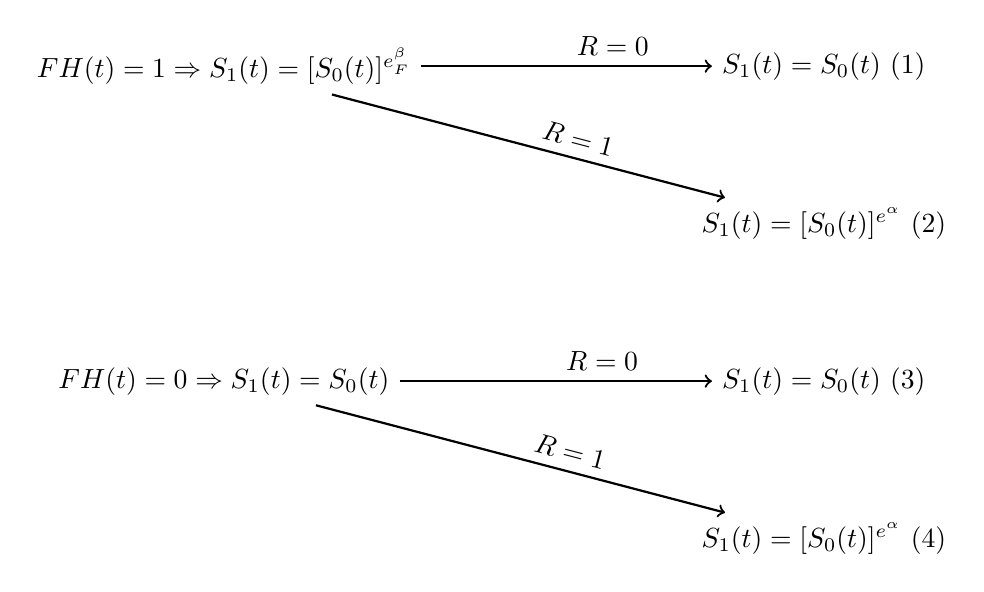
\begin{tikzpicture}[scale=4, node distance={20mm}, thick, main/.style = {draw=none}] 
\node (1) {$S_1(t) = S_0(t)$ (1)}; 
\node (2) [left of=1, node distance=3in]
{$FH(t)=1\Rightarrow S_1(t)=[S_0(t)]^{\text{e}^\beta_F}$};
\node (3) [below of=1] {$S_1(t) = [S_0(t)]^{\text{e}^{\alpha}}$ (2)};
\node (4) [below of=3] {$S_1(t) = S_0(t)$ (3)}; 
\node (5) [left of=4, node distance=3in] {$FH(t)=0\Rightarrow S_1(t)=S_0(t)$};
\node (6) [below of=4] {$S_1(t) = [S_0(t)]^{\text{e}^{\alpha}}$ (4)}; 
%\node[main] (8) [right of (6)]{\textcolor{red}{misspefication}};
\draw[->] (2) -- node[above right, sloped, midway] {$R=0$} (1);
\draw[->] (2) -- node[above right, sloped, midway] {$R=1$} (3); 
\draw[->] (5) -- node[above right, sloped, midway] {$R=0$}(4);
\draw[->] (5) -- node[above right, sloped, midway] {$R=1$}(6); 
\end{tikzpicture}
\end{center}

We find model misspecification in scenarios (1) and (4). If we are in the case where all the high-risk women are well classified in the high-risk group then specifications (2) and (3) are well identified and in particular, in specification (2) the parameter estimation process of $\beta_F$ leads to correct identification of the true parameter $\alpha$. 
\section{Agreement probabilities}\label{appendix:f}
We compute the probabilities of agreement $P(FH=R\mid R=1), \ P(FH=R\mid R=0)$ and the more interesting probabilities of correct classification and misclassification: \begin{align*}
    &P(FH=1\mid R=1) = p_{11} \\
    &P(FH=0\mid R=0) = p_{00} \\
    &P(FH=1\mid R=0) = p_{10} \\
    &P(FH=0\mid R=1) = 1 - p_{11}
\end{align*}
First, we compute the probability that $FH(t) = 0$ so that we have a first measure of how well the indicator represents the true latent risk group membership: \begin{align*}
    P(FH_i(b_i+t) = 0) &\overset{\perp}{=} P(t_{i_g} \ge t + 60)P(t_{i_m} \ge t + 30)P(t_{i_s} \ge t) \\ 
    &= S_{T_{i_g}}(t+60)S_{T_{i_m}}(t+30)S_{T_{i_s}}(t).
\end{align*}
    \footnote{We leave distinct survival functions for family members $S_{T_{i_g}}$ $S_{T_{i_m}}$, $S_{T_{i_s}}$ so that we can involve the improved survival across generations or not. In the generational survival improvement case we obtain the probability $P(FH_i(b_i+t)=0)=[S_{T_i}(t+60)]^{\beta_m^2}[S_{T_i}(t+30)]^{\beta_m} [S_{T_i}(t)]$.}
For simplicity, we start computations from the trivial Exponential model and we recall that there is not a generational survival change so survival functions are $S_{T_{i_g}}=S_{T_{i_m}}=S_{T_{i_s}}=S_{T_i}$. The marginal probability of the indicator in the survival case is: \begin{align*}
    P(FH_i(b_i+t) = 0) =\text{e}^{-\lambda(3t+90)}=\text{e}^{-3\lambda(t+30)}.
\end{align*}
This probability in the cure rate case is: \begin{align*}
    P(FH_i(b_i+t) = 0) =&\left(p+(1-p)\text{e}^{-\lambda^*(t+60)}\right)\left(p+(1-p)\text{e}^{-\lambda^*(t+30)}\right)\cdot \\
    &\cdot\left(p+(1-p)\text{e}^{-\lambda^*t}\right)
\end{align*}
The plot is in Figure \ref{fig:disease 0}.
\begin{figure}[ht]
    \centering
    % \includegraphics{plots/plot_0_disease.png}
    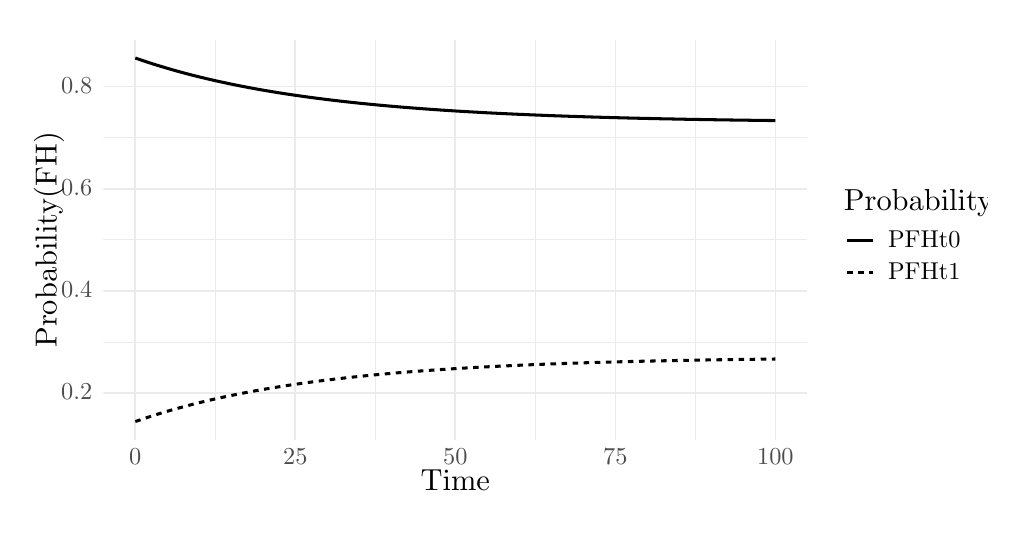
\begin{tikzpicture}[x=1pt,y=1pt, scale=0.8]
\definecolor{fillColor}{RGB}{255,255,255}
\path[use as bounding box,fill=fillColor,fill opacity=0.00] (0,0) rectangle (433.62,216.81);
\begin{scope}
\path[clip] ( 34.16, 30.69) rectangle (352.17,211.31);
\definecolor{drawColor}{gray}{0.92}

\path[draw=drawColor,line width= 0.3pt,line join=round] ( 34.16, 74.85) --
	(352.17, 74.85);

\path[draw=drawColor,line width= 0.3pt,line join=round] ( 34.16,121.00) --
	(352.17,121.00);

\path[draw=drawColor,line width= 0.3pt,line join=round] ( 34.16,167.15) --
	(352.17,167.15);

\path[draw=drawColor,line width= 0.3pt,line join=round] ( 84.75, 30.69) --
	( 84.75,211.31);

\path[draw=drawColor,line width= 0.3pt,line join=round] (157.03, 30.69) --
	(157.03,211.31);

\path[draw=drawColor,line width= 0.3pt,line join=round] (229.30, 30.69) --
	(229.30,211.31);

\path[draw=drawColor,line width= 0.3pt,line join=round] (301.58, 30.69) --
	(301.58,211.31);

\path[draw=drawColor,line width= 0.6pt,line join=round] ( 34.16, 51.77) --
	(352.17, 51.77);

\path[draw=drawColor,line width= 0.6pt,line join=round] ( 34.16, 97.92) --
	(352.17, 97.92);

\path[draw=drawColor,line width= 0.6pt,line join=round] ( 34.16,144.07) --
	(352.17,144.07);

\path[draw=drawColor,line width= 0.6pt,line join=round] ( 34.16,190.23) --
	(352.17,190.23);

\path[draw=drawColor,line width= 0.6pt,line join=round] ( 48.61, 30.69) --
	( 48.61,211.31);

\path[draw=drawColor,line width= 0.6pt,line join=round] (120.89, 30.69) --
	(120.89,211.31);

\path[draw=drawColor,line width= 0.6pt,line join=round] (193.16, 30.69) --
	(193.16,211.31);

\path[draw=drawColor,line width= 0.6pt,line join=round] (265.44, 30.69) --
	(265.44,211.31);

\path[draw=drawColor,line width= 0.6pt,line join=round] (337.72, 30.69) --
	(337.72,211.31);
\definecolor{drawColor}{RGB}{0,0,0}

\path[draw=drawColor,line width= 1.1pt,line join=round] ( 48.61,203.10) --
	( 51.50,202.10) --
	( 54.39,201.14) --
	( 57.28,200.21) --
	( 60.18,199.32) --
	( 63.07,198.46) --
	( 65.96,197.62) --
	( 68.85,196.82) --
	( 71.74,196.04) --
	( 74.63,195.29) --
	( 77.52,194.57) --
	( 80.41,193.87) --
	( 83.30,193.20) --
	( 86.20,192.55) --
	( 89.09,191.92) --
	( 91.98,191.31) --
	( 94.87,190.72) --
	( 97.76,190.16) --
	(100.65,189.61) --
	(103.54,189.08) --
	(106.43,188.57) --
	(109.32,188.08) --
	(112.21,187.60) --
	(115.11,187.14) --
	(118.00,186.70) --
	(120.89,186.27) --
	(123.78,185.86) --
	(126.67,185.46) --
	(129.56,185.07) --
	(132.45,184.70) --
	(135.34,184.33) --
	(138.23,183.99) --
	(141.13,183.65) --
	(144.02,183.32) --
	(146.91,183.01) --
	(149.80,182.70) --
	(152.69,182.41) --
	(155.58,182.13) --
	(158.47,181.85) --
	(161.36,181.59) --
	(164.25,181.33) --
	(167.14,181.08) --
	(170.04,180.84) --
	(172.93,180.61) --
	(175.82,180.39) --
	(178.71,180.17) --
	(181.60,179.96) --
	(184.49,179.76) --
	(187.38,179.56) --
	(190.27,179.37) --
	(193.16,179.19) --
	(196.05,179.01) --
	(198.95,178.84) --
	(201.84,178.68) --
	(204.73,178.52) --
	(207.62,178.36) --
	(210.51,178.21) --
	(213.40,178.07) --
	(216.29,177.93) --
	(219.18,177.80) --
	(222.07,177.67) --
	(224.97,177.54) --
	(227.86,177.42) --
	(230.75,177.30) --
	(233.64,177.19) --
	(236.53,177.08) --
	(239.42,176.97) --
	(242.31,176.87) --
	(245.20,176.77) --
	(248.09,176.67) --
	(250.98,176.58) --
	(253.88,176.49) --
	(256.77,176.40) --
	(259.66,176.32) --
	(262.55,176.24) --
	(265.44,176.16) --
	(268.33,176.08) --
	(271.22,176.01) --
	(274.11,175.94) --
	(277.00,175.87) --
	(279.90,175.80) --
	(282.79,175.74) --
	(285.68,175.67) --
	(288.57,175.61) --
	(291.46,175.56) --
	(294.35,175.50) --
	(297.24,175.44) --
	(300.13,175.39) --
	(303.02,175.34) --
	(305.91,175.29) --
	(308.81,175.24) --
	(311.70,175.20) --
	(314.59,175.15) --
	(317.48,175.11) --
	(320.37,175.07) --
	(323.26,175.03) --
	(326.15,174.99) --
	(329.04,174.95) --
	(331.93,174.92) --
	(334.83,174.88) --
	(337.72,174.85);

\path[draw=drawColor,line width= 1.1pt,dash pattern=on 2pt off 2pt ,line join=round] ( 48.61, 38.90) --
	( 51.50, 39.89) --
	( 54.39, 40.85) --
	( 57.28, 41.78) --
	( 60.18, 42.68) --
	( 63.07, 43.54) --
	( 65.96, 44.37) --
	( 68.85, 45.18) --
	( 71.74, 45.95) --
	( 74.63, 46.70) --
	( 77.52, 47.43) --
	( 80.41, 48.13) --
	( 83.30, 48.80) --
	( 86.20, 49.45) --
	( 89.09, 50.08) --
	( 91.98, 50.69) --
	( 94.87, 51.27) --
	( 97.76, 51.84) --
	(100.65, 52.39) --
	(103.54, 52.91) --
	(106.43, 53.42) --
	(109.32, 53.92) --
	(112.21, 54.39) --
	(115.11, 54.85) --
	(118.00, 55.30) --
	(120.89, 55.72) --
	(123.78, 56.14) --
	(126.67, 56.54) --
	(129.56, 56.93) --
	(132.45, 57.30) --
	(135.34, 57.66) --
	(138.23, 58.01) --
	(141.13, 58.35) --
	(144.02, 58.67) --
	(146.91, 58.99) --
	(149.80, 59.29) --
	(152.69, 59.59) --
	(155.58, 59.87) --
	(158.47, 60.15) --
	(161.36, 60.41) --
	(164.25, 60.67) --
	(167.14, 60.92) --
	(170.04, 61.15) --
	(172.93, 61.39) --
	(175.82, 61.61) --
	(178.71, 61.83) --
	(181.60, 62.04) --
	(184.49, 62.24) --
	(187.38, 62.43) --
	(190.27, 62.62) --
	(193.16, 62.81) --
	(196.05, 62.98) --
	(198.95, 63.15) --
	(201.84, 63.32) --
	(204.73, 63.48) --
	(207.62, 63.63) --
	(210.51, 63.78) --
	(213.40, 63.93) --
	(216.29, 64.06) --
	(219.18, 64.20) --
	(222.07, 64.33) --
	(224.97, 64.46) --
	(227.86, 64.58) --
	(230.75, 64.70) --
	(233.64, 64.81) --
	(236.53, 64.92) --
	(239.42, 65.03) --
	(242.31, 65.13) --
	(245.20, 65.23) --
	(248.09, 65.32) --
	(250.98, 65.42) --
	(253.88, 65.51) --
	(256.77, 65.60) --
	(259.66, 65.68) --
	(262.55, 65.76) --
	(265.44, 65.84) --
	(268.33, 65.92) --
	(271.22, 65.99) --
	(274.11, 66.06) --
	(277.00, 66.13) --
	(279.90, 66.20) --
	(282.79, 66.26) --
	(285.68, 66.32) --
	(288.57, 66.38) --
	(291.46, 66.44) --
	(294.35, 66.50) --
	(297.24, 66.55) --
	(300.13, 66.60) --
	(303.02, 66.65) --
	(305.91, 66.70) --
	(308.81, 66.75) --
	(311.70, 66.80) --
	(314.59, 66.84) --
	(317.48, 66.89) --
	(320.37, 66.93) --
	(323.26, 66.97) --
	(326.15, 67.01) --
	(329.04, 67.04) --
	(331.93, 67.08) --
	(334.83, 67.12) --
	(337.72, 67.15);
\end{scope}
\begin{scope}
\path[clip] (  0.00,  0.00) rectangle (433.62,216.81);
\definecolor{drawColor}{gray}{0.30}

\node[text=drawColor,anchor=base east,inner sep=0pt, outer sep=0pt, scale=  0.88] at ( 29.21, 48.74) {0.2};

\node[text=drawColor,anchor=base east,inner sep=0pt, outer sep=0pt, scale=  0.88] at ( 29.21, 94.89) {0.4};

\node[text=drawColor,anchor=base east,inner sep=0pt, outer sep=0pt, scale=  0.88] at ( 29.21,141.04) {0.6};

\node[text=drawColor,anchor=base east,inner sep=0pt, outer sep=0pt, scale=  0.88] at ( 29.21,187.20) {0.8};
\end{scope}
\begin{scope}
\path[clip] (  0.00,  0.00) rectangle (433.62,216.81);
\definecolor{drawColor}{gray}{0.30}

\node[text=drawColor,anchor=base,inner sep=0pt, outer sep=0pt, scale=  0.88] at ( 48.61, 19.68) {0};

\node[text=drawColor,anchor=base,inner sep=0pt, outer sep=0pt, scale=  0.88] at (120.89, 19.68) {25};

\node[text=drawColor,anchor=base,inner sep=0pt, outer sep=0pt, scale=  0.88] at (193.16, 19.68) {50};

\node[text=drawColor,anchor=base,inner sep=0pt, outer sep=0pt, scale=  0.88] at (265.44, 19.68) {75};

\node[text=drawColor,anchor=base,inner sep=0pt, outer sep=0pt, scale=  0.88] at (337.72, 19.68) {100};
\end{scope}
\begin{scope}
\path[clip] (  0.00,  0.00) rectangle (433.62,216.81);
\definecolor{drawColor}{RGB}{0,0,0}

\node[text=drawColor,anchor=base,inner sep=0pt, outer sep=0pt, scale=  1.10] at (193.16,  7.64) {Time};
\end{scope}
\begin{scope}
\path[clip] (  0.00,  0.00) rectangle (433.62,216.81);
\definecolor{drawColor}{RGB}{0,0,0}

\node[text=drawColor,rotate= 90.00,anchor=base,inner sep=0pt, outer sep=0pt, scale=  1.10] at ( 13.08,121.00) {Probability(FH)};
\end{scope}
\begin{scope}
\path[clip] (  0.00,  0.00) rectangle (433.62,216.81);
\definecolor{drawColor}{RGB}{0,0,0}

\node[text=drawColor,anchor=base west,inner sep=0pt, outer sep=0pt, scale=  1.10] at (368.67,134.41) {Probability};
\end{scope}
\begin{scope}
\path[clip] (  0.00,  0.00) rectangle (433.62,216.81);
\definecolor{drawColor}{RGB}{0,0,0}

\path[draw=drawColor,line width= 1.1pt,line join=round] (370.12,120.62) -- (381.68,120.62);
\end{scope}
\begin{scope}
\path[clip] (  0.00,  0.00) rectangle (433.62,216.81);
\definecolor{drawColor}{RGB}{0,0,0}

\path[draw=drawColor,line width= 1.1pt,dash pattern=on 2pt off 2pt ,line join=round] (370.12,106.16) -- (381.68,106.16);
\end{scope}
\begin{scope}
\path[clip] (  0.00,  0.00) rectangle (433.62,216.81);
\definecolor{drawColor}{RGB}{0,0,0}

\node[text=drawColor,anchor=base west,inner sep=0pt, outer sep=0pt, scale=  0.88] at (388.63,117.59) {PFHt0};
\end{scope}
\begin{scope}
\path[clip] (  0.00,  0.00) rectangle (433.62,216.81);
\definecolor{drawColor}{RGB}{0,0,0}

\node[text=drawColor,anchor=base west,inner sep=0pt, outer sep=0pt, scale=  0.88] at (388.63,103.13) {PFHt1};
\end{scope}
\end{tikzpicture}
    \caption{Probability of FH = 0 (PFHt0) vs Probability of FH = 1 (PFHt1)}
    \label{fig:disease 0}
\end{figure}
The difference between the two indicators can assume the values: $(FH(t) - R) \in \left\{-1, 0, 1\right\}$. We would like to be as close as possible to the scenario with no difference between the indicators. Importantly, $R$ is fixed while $FH(t)$ depends on $t$. 

% We compute the probabilities of the agreement for low and high-risk group membership. The conditional probability of agreement in the low-risk group over the whole $\mathbb{R}^+$ time axis is:

We now compute the probabilities of the agreement for low and high-risk group membership. For the survival case we recall that the hazard function in the low (high) risk group is $\lambda_0(t)$ ($\lambda_1(t)=\alpha\cdot\lambda_0(t)$). keeping in mind that  $\lambda(t\mid R=0)=\lambda_0=\lambda$ and $\lambda(t\mid R=1)=\lambda_1(t)=\beta\lambda_0(t)=\beta\lambda$. But this does not hold in the disease development case. The probability of agreement in the low-risk group over the whole $\mathbb{R}^+$ time axis is: 
\begin{align*}
    %\label{prob_0}
    &P(FH_i(b_i+t) = R_i\mid R_i=0) =\int_0^{\infty}P(FH_i(b_i+t)=0)f_{0}(t)\text{d}t \nonumber \\
    &=\int_0^{\infty}\left(p+(1-p)\text{e}^{-\lambda^*(t+60)}\right)\left(p+(1-p)\text{e}^{-\lambda^*(t+30)}\right)\cdot\\ 
    &\cdot\left(p+(1-p)\text{e}^{-\lambda^*t}\right)(1-p)\lambda^* e^{-\lambda^* t}\text{d}t
\end{align*}
Similarly, we compute the probability of agreement for the high-risk group:
    \begin{align*}
    %\label{prob_1}
    &P(FH_i(b_i+t) = R_i\mid R_i=1) =\int_0^{\infty}P(FH_i(b_i+t)=1)f_{1}(t)\text{d}t \\
    &=\int_0^{\infty}(1 - P(FH_i(b_i+t)=0))f_1(t,\lambda^*)\text{d}t \nonumber \\
    &=\int_0^{\infty}f_1(t,\lambda^*) - P(FH_i(b_i+t)=0)f_1(t,\lambda^*)\text{d}t \nonumber \\
    &=\int_0^{\infty}f_1(t,\lambda^*)\text{d}t - \int_0^{\infty}P(FH_i(b_i+t)=0)f_1(t,\lambda^*)\text{d}t  \\
    &=1 - \int_0^{\infty}P(FH_i(b_i+t)=0)f_1(t,\lambda^*)\text{d}t\nonumber \\
    &=1 - \int_0^{\infty}P(FH_i(b_i+t)=0)(1-\widetilde{p})\left(\dfrac{f^*(t)e^{\alpha}}{1-\widetilde{p}}\right)(p+(1-p)S^*(t))^{e^\alpha-1}\text{d}t \nonumber
\end{align*} 
One would like both probabilities to be large. For the cure rate case, the conditional probability of agreement in the low-risk group over the whole $\mathbb{R}^+$ time axis is: 
\begin{align*}
    % \label{formula:1_2}
    P(FH_i(b_i+t) = R_i\mid R_i=0) &=\int_0^{\infty}P(FH_i(b_i+t)=0)f_0(t)\text{d}t 
\end{align*} Easily, we obtain the conditional probability of agreement for the high-risk group:
\begin{align*}
    % \label{formula:1_3}
    P(F H_i(b_i+t) = R_i\mid R_i=1)  &=\int_0^{\infty}P(F H_i(b_i+t)=1)f_1(t)\text{d}t
\end{align*} 
We can also analyse the misclassification probabilities (note that we implicitly assume that the proportion of high-risk families $P(R=1)=h$ is constant over time).
For the cure rate case the conditional correct classification probabilities are: \begin{align*}
    % \label{probs_final}
    &P(FH_i(t)=0\mid R_i=0)=S_0(t+60)S_0(t+30)S_0(t) \\
    &=(p+(1-p)S^*(t+60)) (p+(1-p)S^*(t+30)) (p+(1-p)S^*(t)) \\
    &=(p+(1-p)e^{-\lambda^*(t+60)}) (p+(1-p)e^{-\lambda^*(t+30)}) (p+(1-p)e^{-\lambda^*(t)}) \\
    &P(FH_i(t)=0\mid R_i=1) = S_1(t+60)S_1(t+30)S_1(t) \\
    &=(S_0(t+60)S_0(t+30)S_0(t))^{e^\alpha} \\
    &=((p+(1-p)e^{-\lambda^*(t+60)}) (p+(1-p)e^{-\lambda^*(t+30)}) (p+(1-p)e^{-\lambda^*(t)}))^{e^\alpha}
\end{align*} 
Clearly, \begin{align*}
    &S_0(t) = p+(1-p)e^{-\lambda^*(t)} \\
    &S_1(t) = (p+(1-p)e^{-\lambda^*(t)})^{e^\alpha}  \\
    &P(FH_i(t)=1\mid R_i=0) = 1 - S_0(t+60)S_0(t+30)S_0(t) \\
    &P(FH_i(t)=1\mid R_i=1) = 1 - S_1(t+60)S_1(t+30)S_1(t)
\end{align*} 
A graphical visualization of these probabilities is illustrated in Figure \ref{fig:disease 1}. 
\begin{figure}[ht]
    \centering
    % \includegraphics{plots/plot_1_disease.png}
    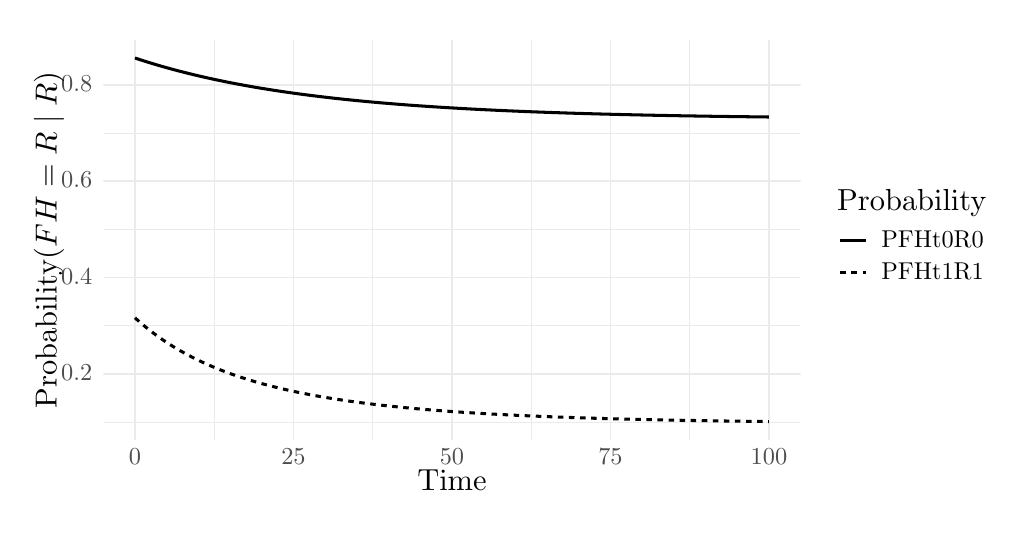
\begin{tikzpicture}[x=1pt,y=1pt,scale=0.8]
\definecolor{fillColor}{RGB}{255,255,255}
\path[use as bounding box,fill=fillColor,fill opacity=0.00] (0,0) rectangle (433.62,216.81);
\begin{scope}
\path[clip] ( 34.16, 30.69) rectangle (349.14,211.31);
\definecolor{drawColor}{gray}{0.92}

\path[draw=drawColor,line width= 0.3pt,line join=round] ( 34.16, 38.66) --
	(349.14, 38.66);

\path[draw=drawColor,line width= 0.3pt,line join=round] ( 34.16, 82.17) --
	(349.14, 82.17);

\path[draw=drawColor,line width= 0.3pt,line join=round] ( 34.16,125.69) --
	(349.14,125.69);

\path[draw=drawColor,line width= 0.3pt,line join=round] ( 34.16,169.20) --
	(349.14,169.20);

\path[draw=drawColor,line width= 0.3pt,line join=round] ( 84.27, 30.69) --
	( 84.27,211.31);

\path[draw=drawColor,line width= 0.3pt,line join=round] (155.86, 30.69) --
	(155.86,211.31);

\path[draw=drawColor,line width= 0.3pt,line join=round] (227.44, 30.69) --
	(227.44,211.31);

\path[draw=drawColor,line width= 0.3pt,line join=round] (299.03, 30.69) --
	(299.03,211.31);

\path[draw=drawColor,line width= 0.6pt,line join=round] ( 34.16, 60.41) --
	(349.14, 60.41);

\path[draw=drawColor,line width= 0.6pt,line join=round] ( 34.16,103.93) --
	(349.14,103.93);

\path[draw=drawColor,line width= 0.6pt,line join=round] ( 34.16,147.45) --
	(349.14,147.45);

\path[draw=drawColor,line width= 0.6pt,line join=round] ( 34.16,190.96) --
	(349.14,190.96);

\path[draw=drawColor,line width= 0.6pt,line join=round] ( 48.47, 30.69) --
	( 48.47,211.31);

\path[draw=drawColor,line width= 0.6pt,line join=round] (120.06, 30.69) --
	(120.06,211.31);

\path[draw=drawColor,line width= 0.6pt,line join=round] (191.65, 30.69) --
	(191.65,211.31);

\path[draw=drawColor,line width= 0.6pt,line join=round] (263.24, 30.69) --
	(263.24,211.31);

\path[draw=drawColor,line width= 0.6pt,line join=round] (334.82, 30.69) --
	(334.82,211.31);
\definecolor{drawColor}{RGB}{0,0,0}

\path[draw=drawColor,line width= 1.1pt,line join=round] ( 48.47,203.10) --
	( 51.34,202.16) --
	( 54.20,201.25) --
	( 57.06,200.38) --
	( 59.93,199.54) --
	( 62.79,198.72) --
	( 65.65,197.94) --
	( 68.52,197.18) --
	( 71.38,196.45) --
	( 74.25,195.74) --
	( 77.11,195.06) --
	( 79.97,194.40) --
	( 82.84,193.76) --
	( 85.70,193.15) --
	( 88.56,192.56) --
	( 91.43,191.98) --
	( 94.29,191.43) --
	( 97.15,190.90) --
	(100.02,190.38) --
	(102.88,189.88) --
	(105.74,189.40) --
	(108.61,188.94) --
	(111.47,188.49) --
	(114.33,188.06) --
	(117.20,187.64) --
	(120.06,187.23) --
	(122.92,186.84) --
	(125.79,186.46) --
	(128.65,186.10) --
	(131.52,185.75) --
	(134.38,185.41) --
	(137.24,185.08) --
	(140.11,184.76) --
	(142.97,184.45) --
	(145.83,184.16) --
	(148.70,183.87) --
	(151.56,183.59) --
	(154.42,183.32) --
	(157.29,183.06) --
	(160.15,182.81) --
	(163.01,182.57) --
	(165.88,182.34) --
	(168.74,182.11) --
	(171.60,181.89) --
	(174.47,181.68) --
	(177.33,181.48) --
	(180.19,181.28) --
	(183.06,181.09) --
	(185.92,180.91) --
	(188.79,180.73) --
	(191.65,180.56) --
	(194.51,180.39) --
	(197.38,180.23) --
	(200.24,180.07) --
	(203.10,179.92) --
	(205.97,179.78) --
	(208.83,179.64) --
	(211.69,179.50) --
	(214.56,179.37) --
	(217.42,179.24) --
	(220.28,179.12) --
	(223.15,179.00) --
	(226.01,178.88) --
	(228.87,178.77) --
	(231.74,178.67) --
	(234.60,178.56) --
	(237.46,178.46) --
	(240.33,178.37) --
	(243.19,178.27) --
	(246.06,178.18) --
	(248.92,178.09) --
	(251.78,178.01) --
	(254.65,177.93) --
	(257.51,177.85) --
	(260.37,177.77) --
	(263.24,177.70) --
	(266.10,177.62) --
	(268.96,177.55) --
	(271.83,177.49) --
	(274.69,177.42) --
	(277.55,177.36) --
	(280.42,177.30) --
	(283.28,177.24) --
	(286.14,177.18) --
	(289.01,177.13) --
	(291.87,177.08) --
	(294.73,177.02) --
	(297.60,176.97) --
	(300.46,176.93) --
	(303.33,176.88) --
	(306.19,176.84) --
	(309.05,176.79) --
	(311.92,176.75) --
	(314.78,176.71) --
	(317.64,176.67) --
	(320.51,176.63) --
	(323.37,176.60) --
	(326.23,176.56) --
	(329.10,176.53) --
	(331.96,176.49) --
	(334.82,176.46);

\path[draw=drawColor,line width= 1.1pt,dash pattern=on 2pt off 2pt ,line join=round] ( 48.47, 85.74) --
	( 51.34, 83.22) --
	( 54.20, 80.86) --
	( 57.06, 78.65) --
	( 59.93, 76.58) --
	( 62.79, 74.64) --
	( 65.65, 72.82) --
	( 68.52, 71.11) --
	( 71.38, 69.51) --
	( 74.25, 68.00) --
	( 77.11, 66.57) --
	( 79.97, 65.23) --
	( 82.84, 63.97) --
	( 85.70, 62.78) --
	( 88.56, 61.65) --
	( 91.43, 60.58) --
	( 94.29, 59.57) --
	( 97.15, 58.62) --
	(100.02, 57.71) --
	(102.88, 56.85) --
	(105.74, 56.04) --
	(108.61, 55.27) --
	(111.47, 54.54) --
	(114.33, 53.84) --
	(117.20, 53.18) --
	(120.06, 52.55) --
	(122.92, 51.95) --
	(125.79, 51.38) --
	(128.65, 50.83) --
	(131.52, 50.31) --
	(134.38, 49.82) --
	(137.24, 49.35) --
	(140.11, 48.90) --
	(142.97, 48.46) --
	(145.83, 48.05) --
	(148.70, 47.66) --
	(151.56, 47.29) --
	(154.42, 46.93) --
	(157.29, 46.58) --
	(160.15, 46.25) --
	(163.01, 45.94) --
	(165.88, 45.64) --
	(168.74, 45.35) --
	(171.60, 45.07) --
	(174.47, 44.81) --
	(177.33, 44.55) --
	(180.19, 44.31) --
	(183.06, 44.07) --
	(185.92, 43.85) --
	(188.79, 43.63) --
	(191.65, 43.43) --
	(194.51, 43.23) --
	(197.38, 43.04) --
	(200.24, 42.85) --
	(203.10, 42.68) --
	(205.97, 42.51) --
	(208.83, 42.34) --
	(211.69, 42.19) --
	(214.56, 42.04) --
	(217.42, 41.89) --
	(220.28, 41.75) --
	(223.15, 41.62) --
	(226.01, 41.49) --
	(228.87, 41.37) --
	(231.74, 41.25) --
	(234.60, 41.13) --
	(237.46, 41.02) --
	(240.33, 40.91) --
	(243.19, 40.81) --
	(246.06, 40.71) --
	(248.92, 40.61) --
	(251.78, 40.52) --
	(254.65, 40.43) --
	(257.51, 40.35) --
	(260.37, 40.27) --
	(263.24, 40.19) --
	(266.10, 40.11) --
	(268.96, 40.04) --
	(271.83, 39.96) --
	(274.69, 39.90) --
	(277.55, 39.83) --
	(280.42, 39.77) --
	(283.28, 39.70) --
	(286.14, 39.64) --
	(289.01, 39.59) --
	(291.87, 39.53) --
	(294.73, 39.48) --
	(297.60, 39.43) --
	(300.46, 39.38) --
	(303.33, 39.33) --
	(306.19, 39.28) --
	(309.05, 39.24) --
	(311.92, 39.19) --
	(314.78, 39.15) --
	(317.64, 39.11) --
	(320.51, 39.07) --
	(323.37, 39.03) --
	(326.23, 39.00) --
	(329.10, 38.96) --
	(331.96, 38.93) --
	(334.82, 38.90);
\end{scope}
\begin{scope}
\path[clip] (  0.00,  0.00) rectangle (433.62,216.81);
\definecolor{drawColor}{gray}{0.30}

\node[text=drawColor,anchor=base east,inner sep=0pt, outer sep=0pt, scale=  0.88] at ( 29.21, 57.38) {0.2};

\node[text=drawColor,anchor=base east,inner sep=0pt, outer sep=0pt, scale=  0.88] at ( 29.21,100.90) {0.4};

\node[text=drawColor,anchor=base east,inner sep=0pt, outer sep=0pt, scale=  0.88] at ( 29.21,144.42) {0.6};

\node[text=drawColor,anchor=base east,inner sep=0pt, outer sep=0pt, scale=  0.88] at ( 29.21,187.93) {0.8};
\end{scope}
\begin{scope}
\path[clip] (  0.00,  0.00) rectangle (433.62,216.81);
\definecolor{drawColor}{gray}{0.30}

\node[text=drawColor,anchor=base,inner sep=0pt, outer sep=0pt, scale=  0.88] at ( 48.47, 19.68) {0};

\node[text=drawColor,anchor=base,inner sep=0pt, outer sep=0pt, scale=  0.88] at (120.06, 19.68) {25};

\node[text=drawColor,anchor=base,inner sep=0pt, outer sep=0pt, scale=  0.88] at (191.65, 19.68) {50};

\node[text=drawColor,anchor=base,inner sep=0pt, outer sep=0pt, scale=  0.88] at (263.24, 19.68) {75};

\node[text=drawColor,anchor=base,inner sep=0pt, outer sep=0pt, scale=  0.88] at (334.82, 19.68) {100};
\end{scope}
\begin{scope}
\path[clip] (  0.00,  0.00) rectangle (433.62,216.81);
\definecolor{drawColor}{RGB}{0,0,0}

\node[text=drawColor,anchor=base,inner sep=0pt, outer sep=0pt, scale=  1.10] at (191.65,  7.64) {Time};
\end{scope}
\begin{scope}
\path[clip] (  0.00,  0.00) rectangle (433.62,216.81);
\definecolor{drawColor}{RGB}{0,0,0}

\node[text=drawColor,rotate= 90.00,anchor=base,inner sep=0pt, outer sep=0pt, scale=  1.10] at ( 13.08,121.00) {Probability($FH = R\mid R$)};
\end{scope}
\begin{scope}
\path[clip] (  0.00,  0.00) rectangle (433.62,216.81);
\definecolor{drawColor}{RGB}{0,0,0}

\node[text=drawColor,anchor=base west,inner sep=0pt, outer sep=0pt, scale=  1.10] at (365.64,134.41) {Probability};
\end{scope}
\begin{scope}
\path[clip] (  0.00,  0.00) rectangle (433.62,216.81);
\definecolor{drawColor}{RGB}{0,0,0}

\path[draw=drawColor,line width= 1.1pt,line join=round] (367.09,120.62) -- (378.65,120.62);
\end{scope}
\begin{scope}
\path[clip] (  0.00,  0.00) rectangle (433.62,216.81);
\definecolor{drawColor}{RGB}{0,0,0}

\path[draw=drawColor,line width= 1.1pt,dash pattern=on 2pt off 2pt ,line join=round] (367.09,106.16) -- (378.65,106.16);
\end{scope}
\begin{scope}
\path[clip] (  0.00,  0.00) rectangle (433.62,216.81);
\definecolor{drawColor}{RGB}{0,0,0}

\node[text=drawColor,anchor=base west,inner sep=0pt, outer sep=0pt, scale=  0.88] at (385.60,117.59) {PFHt0R0};
\end{scope}
\begin{scope}
\path[clip] (  0.00,  0.00) rectangle (433.62,216.81);
\definecolor{drawColor}{RGB}{0,0,0}

\node[text=drawColor,anchor=base west,inner sep=0pt, outer sep=0pt, scale=  0.88] at (385.60,103.13) {PFHt1R1};
\end{scope}
\end{tikzpicture}
    \caption{Probability of $FH = 0$ conditional to $R = 0$ (PFHt0R0) vs. Probability of $(FH = 1$ conditional to $R=1$ (PFHt1R1)}
    \label{fig:disease 1}
\end{figure}
We also compute the inverse probabilities of correct classification only for the survival case, i.e.: (i) $P(R_i=0\mid FH_i(t)=0)$ and (ii) $P(R_i=1\mid FH_i(t)=1)$. These are: \begin{align*}
    &(i) \ P(R_i = 0\mid FH_i(t)=0) = \dfrac{P(FH_i(t)=0\mid R_i=0)P(R_i=0)}{P(FH_i(t)=0)} \\
    &= \dfrac{P(FH_i(t)=0\mid R_i=0)(1-h)}{P(FH_i(t)=0\mid R_i=0)(1-h) +P(FH_i(t)=0\mid R_i=1)h} \\
    &= \dfrac{f(t,p,\lambda^*)(1-h)}{f(t,p,\lambda^*)(1-h)+\left(f(t,p,\lambda^*)^{e^\alpha} \right)h}
\end{align*} and \begin{align*}
    &(ii) \ P(R_i = 1\mid FH_i(t)=1) = \dfrac{P(FH_i(t)=1\mid R_i=1)P(R_i=1)}{P(FH_i(t)=1)}  \\
    &= \dfrac{P(FH_i(t)=1\mid R_i=1)h}{P(FH_i(t)=1\mid R_i=1)h +P(FH_i(t)=1\mid R_i=0)(1-h) } \\
    &=\dfrac{(1-f(t,p,\lambda^*)^{e^\alpha})h}{(1-f(t,p,\lambda^*)^{e^\alpha})h+\left(1-f(t,p,\lambda^*)\right)(1-h)}
\end{align*}
with $f(t,p,\lambda^*) = (p+(1-p)e^{-\lambda^*(t+60)}) (p+(1-p)e^{-\lambda^*(t+30)}) (p+(1-p)e^{-\lambda^*(t)})$
With these probabilities, we describe the distribution of the measurement error when using the observed $FH(t)$ instead of $R$ in the observed data model. A graphical representation of the trend of these probabilities for the fixed values $\lambda=1/90$, $\alpha=2$, $h=0.7$ is illustrated in figure \ref{fig:disease 2}. \begin{figure}[ht]
    \centering
    % \includegraphics{plots/plot_2_disease.png}
    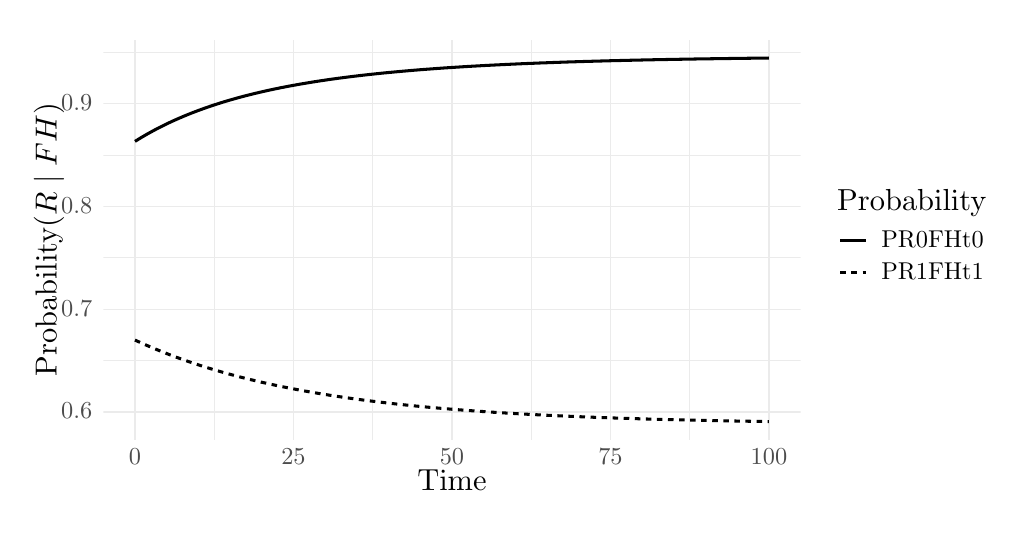
\begin{tikzpicture}[x=1pt,y=1pt,scale=0.8]
\definecolor{fillColor}{RGB}{255,255,255}
\path[use as bounding box,fill=fillColor,fill opacity=0.00] (0,0) rectangle (433.62,216.81);
\begin{scope}
\path[clip] ( 34.16, 30.69) rectangle (349.14,211.31);
\definecolor{drawColor}{gray}{0.92}

\path[draw=drawColor,line width= 0.3pt,line join=round] ( 34.16, 66.34) --
	(349.14, 66.34);

\path[draw=drawColor,line width= 0.3pt,line join=round] ( 34.16,112.82) --
	(349.14,112.82);

\path[draw=drawColor,line width= 0.3pt,line join=round] ( 34.16,159.31) --
	(349.14,159.31);

\path[draw=drawColor,line width= 0.3pt,line join=round] ( 34.16,205.79) --
	(349.14,205.79);

\path[draw=drawColor,line width= 0.3pt,line join=round] ( 84.27, 30.69) --
	( 84.27,211.31);

\path[draw=drawColor,line width= 0.3pt,line join=round] (155.86, 30.69) --
	(155.86,211.31);

\path[draw=drawColor,line width= 0.3pt,line join=round] (227.44, 30.69) --
	(227.44,211.31);

\path[draw=drawColor,line width= 0.3pt,line join=round] (299.03, 30.69) --
	(299.03,211.31);

\path[draw=drawColor,line width= 0.6pt,line join=round] ( 34.16, 43.10) --
	(349.14, 43.10);

\path[draw=drawColor,line width= 0.6pt,line join=round] ( 34.16, 89.58) --
	(349.14, 89.58);

\path[draw=drawColor,line width= 0.6pt,line join=round] ( 34.16,136.07) --
	(349.14,136.07);

\path[draw=drawColor,line width= 0.6pt,line join=round] ( 34.16,182.55) --
	(349.14,182.55);

\path[draw=drawColor,line width= 0.6pt,line join=round] ( 48.47, 30.69) --
	( 48.47,211.31);

\path[draw=drawColor,line width= 0.6pt,line join=round] (120.06, 30.69) --
	(120.06,211.31);

\path[draw=drawColor,line width= 0.6pt,line join=round] (191.65, 30.69) --
	(191.65,211.31);

\path[draw=drawColor,line width= 0.6pt,line join=round] (263.24, 30.69) --
	(263.24,211.31);

\path[draw=drawColor,line width= 0.6pt,line join=round] (334.82, 30.69) --
	(334.82,211.31);
\definecolor{drawColor}{RGB}{0,0,0}

\path[draw=drawColor,line width= 1.1pt,line join=round] ( 48.47,165.45) --
	( 51.34,167.21) --
	( 54.20,168.87) --
	( 57.06,170.44) --
	( 59.93,171.93) --
	( 62.79,173.35) --
	( 65.65,174.69) --
	( 68.52,175.96) --
	( 71.38,177.17) --
	( 74.25,178.32) --
	( 77.11,179.41) --
	( 79.97,180.45) --
	( 82.84,181.44) --
	( 85.70,182.38) --
	( 88.56,183.28) --
	( 91.43,184.13) --
	( 94.29,184.94) --
	( 97.15,185.72) --
	(100.02,186.46) --
	(102.88,187.16) --
	(105.74,187.83) --
	(108.61,188.48) --
	(111.47,189.09) --
	(114.33,189.68) --
	(117.20,190.24) --
	(120.06,190.77) --
	(122.92,191.28) --
	(125.79,191.77) --
	(128.65,192.24) --
	(131.52,192.69) --
	(134.38,193.12) --
	(137.24,193.53) --
	(140.11,193.93) --
	(142.97,194.30) --
	(145.83,194.67) --
	(148.70,195.01) --
	(151.56,195.35) --
	(154.42,195.67) --
	(157.29,195.97) --
	(160.15,196.27) --
	(163.01,196.55) --
	(165.88,196.82) --
	(168.74,197.08) --
	(171.60,197.33) --
	(174.47,197.58) --
	(177.33,197.81) --
	(180.19,198.03) --
	(183.06,198.24) --
	(185.92,198.45) --
	(188.79,198.65) --
	(191.65,198.84) --
	(194.51,199.02) --
	(197.38,199.20) --
	(200.24,199.37) --
	(203.10,199.53) --
	(205.97,199.69) --
	(208.83,199.84) --
	(211.69,199.98) --
	(214.56,200.12) --
	(217.42,200.26) --
	(220.28,200.39) --
	(223.15,200.52) --
	(226.01,200.64) --
	(228.87,200.75) --
	(231.74,200.87) --
	(234.60,200.97) --
	(237.46,201.08) --
	(240.33,201.18) --
	(243.19,201.28) --
	(246.06,201.37) --
	(248.92,201.46) --
	(251.78,201.55) --
	(254.65,201.63) --
	(257.51,201.71) --
	(260.37,201.79) --
	(263.24,201.87) --
	(266.10,201.94) --
	(268.96,202.01) --
	(271.83,202.08) --
	(274.69,202.14) --
	(277.55,202.21) --
	(280.42,202.27) --
	(283.28,202.33) --
	(286.14,202.38) --
	(289.01,202.44) --
	(291.87,202.49) --
	(294.73,202.54) --
	(297.60,202.59) --
	(300.46,202.64) --
	(303.33,202.69) --
	(306.19,202.73) --
	(309.05,202.77) --
	(311.92,202.81) --
	(314.78,202.85) --
	(317.64,202.89) --
	(320.51,202.93) --
	(323.37,202.97) --
	(326.23,203.00) --
	(329.10,203.04) --
	(331.96,203.07) --
	(334.82,203.10);

\path[draw=drawColor,line width= 1.1pt,dash pattern=on 2pt off 2pt ,line join=round] ( 48.47, 75.70) --
	( 51.34, 74.39) --
	( 54.20, 73.13) --
	( 57.06, 71.92) --
	( 59.93, 70.75) --
	( 62.79, 69.61) --
	( 65.65, 68.52) --
	( 68.52, 67.46) --
	( 71.38, 66.44) --
	( 74.25, 65.46) --
	( 77.11, 64.51) --
	( 79.97, 63.59) --
	( 82.84, 62.71) --
	( 85.70, 61.85) --
	( 88.56, 61.03) --
	( 91.43, 60.23) --
	( 94.29, 59.47) --
	( 97.15, 58.72) --
	(100.02, 58.01) --
	(102.88, 57.32) --
	(105.74, 56.65) --
	(108.61, 56.01) --
	(111.47, 55.39) --
	(114.33, 54.78) --
	(117.20, 54.21) --
	(120.06, 53.65) --
	(122.92, 53.11) --
	(125.79, 52.58) --
	(128.65, 52.08) --
	(131.52, 51.59) --
	(134.38, 51.12) --
	(137.24, 50.67) --
	(140.11, 50.23) --
	(142.97, 49.81) --
	(145.83, 49.40) --
	(148.70, 49.00) --
	(151.56, 48.62) --
	(154.42, 48.25) --
	(157.29, 47.90) --
	(160.15, 47.56) --
	(163.01, 47.22) --
	(165.88, 46.90) --
	(168.74, 46.59) --
	(171.60, 46.29) --
	(174.47, 46.00) --
	(177.33, 45.72) --
	(180.19, 45.45) --
	(183.06, 45.19) --
	(185.92, 44.94) --
	(188.79, 44.70) --
	(191.65, 44.46) --
	(194.51, 44.24) --
	(197.38, 44.02) --
	(200.24, 43.80) --
	(203.10, 43.60) --
	(205.97, 43.40) --
	(208.83, 43.21) --
	(211.69, 43.02) --
	(214.56, 42.84) --
	(217.42, 42.67) --
	(220.28, 42.50) --
	(223.15, 42.34) --
	(226.01, 42.18) --
	(228.87, 42.03) --
	(231.74, 41.89) --
	(234.60, 41.75) --
	(237.46, 41.61) --
	(240.33, 41.48) --
	(243.19, 41.35) --
	(246.06, 41.23) --
	(248.92, 41.11) --
	(251.78, 40.99) --
	(254.65, 40.88) --
	(257.51, 40.77) --
	(260.37, 40.67) --
	(263.24, 40.57) --
	(266.10, 40.47) --
	(268.96, 40.38) --
	(271.83, 40.29) --
	(274.69, 40.20) --
	(277.55, 40.11) --
	(280.42, 40.03) --
	(283.28, 39.95) --
	(286.14, 39.87) --
	(289.01, 39.80) --
	(291.87, 39.73) --
	(294.73, 39.66) --
	(297.60, 39.59) --
	(300.46, 39.53) --
	(303.33, 39.46) --
	(306.19, 39.40) --
	(309.05, 39.34) --
	(311.92, 39.29) --
	(314.78, 39.23) --
	(317.64, 39.18) --
	(320.51, 39.13) --
	(323.37, 39.08) --
	(326.23, 39.03) --
	(329.10, 38.98) --
	(331.96, 38.94) --
	(334.82, 38.90);
\end{scope}
\begin{scope}
\path[clip] (  0.00,  0.00) rectangle (433.62,216.81);
\definecolor{drawColor}{gray}{0.30}

\node[text=drawColor,anchor=base east,inner sep=0pt, outer sep=0pt, scale=  0.88] at ( 29.21, 40.07) {0.6};

\node[text=drawColor,anchor=base east,inner sep=0pt, outer sep=0pt, scale=  0.88] at ( 29.21, 86.55) {0.7};

\node[text=drawColor,anchor=base east,inner sep=0pt, outer sep=0pt, scale=  0.88] at ( 29.21,133.04) {0.8};

\node[text=drawColor,anchor=base east,inner sep=0pt, outer sep=0pt, scale=  0.88] at ( 29.21,179.52) {0.9};
\end{scope}
\begin{scope}
\path[clip] (  0.00,  0.00) rectangle (433.62,216.81);
\definecolor{drawColor}{gray}{0.30}

\node[text=drawColor,anchor=base,inner sep=0pt, outer sep=0pt, scale=  0.88] at ( 48.47, 19.68) {0};

\node[text=drawColor,anchor=base,inner sep=0pt, outer sep=0pt, scale=  0.88] at (120.06, 19.68) {25};

\node[text=drawColor,anchor=base,inner sep=0pt, outer sep=0pt, scale=  0.88] at (191.65, 19.68) {50};

\node[text=drawColor,anchor=base,inner sep=0pt, outer sep=0pt, scale=  0.88] at (263.24, 19.68) {75};

\node[text=drawColor,anchor=base,inner sep=0pt, outer sep=0pt, scale=  0.88] at (334.82, 19.68) {100};
\end{scope}
\begin{scope}
\path[clip] (  0.00,  0.00) rectangle (433.62,216.81);
\definecolor{drawColor}{RGB}{0,0,0}

\node[text=drawColor,anchor=base,inner sep=0pt, outer sep=0pt, scale=  1.10] at (191.65,  7.64) {Time};
\end{scope}
\begin{scope}
\path[clip] (  0.00,  0.00) rectangle (433.62,216.81);
\definecolor{drawColor}{RGB}{0,0,0}

\node[text=drawColor,rotate= 90.00,anchor=base,inner sep=0pt, outer sep=0pt, scale=  1.10] at ( 13.08,121.00) {Probability($R\mid FH$)};
\end{scope}
\begin{scope}
\path[clip] (  0.00,  0.00) rectangle (433.62,216.81);
\definecolor{drawColor}{RGB}{0,0,0}

\node[text=drawColor,anchor=base west,inner sep=0pt, outer sep=0pt, scale=  1.10] at (365.64,134.41) {Probability};
\end{scope}
\begin{scope}
\path[clip] (  0.00,  0.00) rectangle (433.62,216.81);
\definecolor{drawColor}{RGB}{0,0,0}

\path[draw=drawColor,line width= 1.1pt,line join=round] (367.09,120.62) -- (378.65,120.62);
\end{scope}
\begin{scope}
\path[clip] (  0.00,  0.00) rectangle (433.62,216.81);
\definecolor{drawColor}{RGB}{0,0,0}

\path[draw=drawColor,line width= 1.1pt,dash pattern=on 2pt off 2pt ,line join=round] (367.09,106.16) -- (378.65,106.16);
\end{scope}
\begin{scope}
\path[clip] (  0.00,  0.00) rectangle (433.62,216.81);
\definecolor{drawColor}{RGB}{0,0,0}

\node[text=drawColor,anchor=base west,inner sep=0pt, outer sep=0pt, scale=  0.88] at (385.60,117.59) {PR0FHt0};
\end{scope}
\begin{scope}
\path[clip] (  0.00,  0.00) rectangle (433.62,216.81);
\definecolor{drawColor}{RGB}{0,0,0}

\node[text=drawColor,anchor=base west,inner sep=0pt, outer sep=0pt, scale=  0.88] at (385.60,103.13) {PR1FHt1};
\end{scope}
\end{tikzpicture}
    \caption{Probability of $R=0$ conditional to $FH=0$ (PR0FHt0) vs. Probability of $R=1$ conditional to $FH=1$ (PR1FHt1)}
    \label{fig:disease 2}
\end{figure}
\newpage
\section{Agreement probabilities}
\label{appendix:e}
We compute the probabilities of agreement $P(FH=R\mid R=1), \ P(FH=R\mid R=0)$ and the more interesting probabilities of correct classification and misclassification: \begin{align*}
    &P(FH=1\mid R=1) = p_{11} \\
    &P(FH=0\mid R=0) = p_{00} \\
    &P(FH=1\mid R=0) = p_{10} \\
    &P(FH=0\mid R=1) = 1 - p_{11}
\end{align*}
First, we compute the probability that $FH(t) = 0$ so that we have a first measure of how well the indicator represents the true latent risk group membership: \begin{align*}
    P(FH_i(b_i+t) = 0) &\overset{\perp}{=} P(t_{i_g} \ge t + 60)P(t_{i_m} \ge t + 30)P(t_{i_s} \ge t) \\ 
    &= S_{T_{i_g}}(t+60)S_{T_{i_m}}(t+30)S_{T_{i_s}}(t).
\end{align*}
    \footnote{We leave distinct survival functions for family members $S_{T_{i_g}}$ $S_{T_{i_m}}$, $S_{T_{i_s}}$ so that we can involve the improved survival across generations or not. In the generational survival improvement case we obtain the probability $P(FH_i(b_i+t)=0)=[S_{T_i}(t+60)]^{\beta_m^2}[S_{T_i}(t+30)]^{\beta_m} [S_{T_i}(t)]$.}
For simplicity, we start computations from the trivial Exponential model and we recall that there is not a generational survival change so survival functions are $S_{T_{i_g}}=S_{T_{i_m}}=S_{T_{i_s}}=S_{T_i}$. The marginal probability of the indicator in the survival case is: \begin{align*}
    P(FH_i(b_i+t) = 0) =\text{e}^{-\lambda(3t+90)}=\text{e}^{-3\lambda(t+30)}.
\end{align*}
This probability in the cure rate case is: \begin{align*}
    P(FH_i(b_i+t) = 0) =\left(p+(1-p)\text{e}^{-\lambda^*(t+60)}\right)\left(p+(1-p)\text{e}^{-\lambda^*(t+30)}\right)\left(p+(1-p)\text{e}^{-\lambda^*t}\right)
\end{align*}
The plot is in Figure \ref{fig:disease 0}.
\begin{figure}[ht]
    \centering
    % \includegraphics{plots/plot_0_disease.png}
    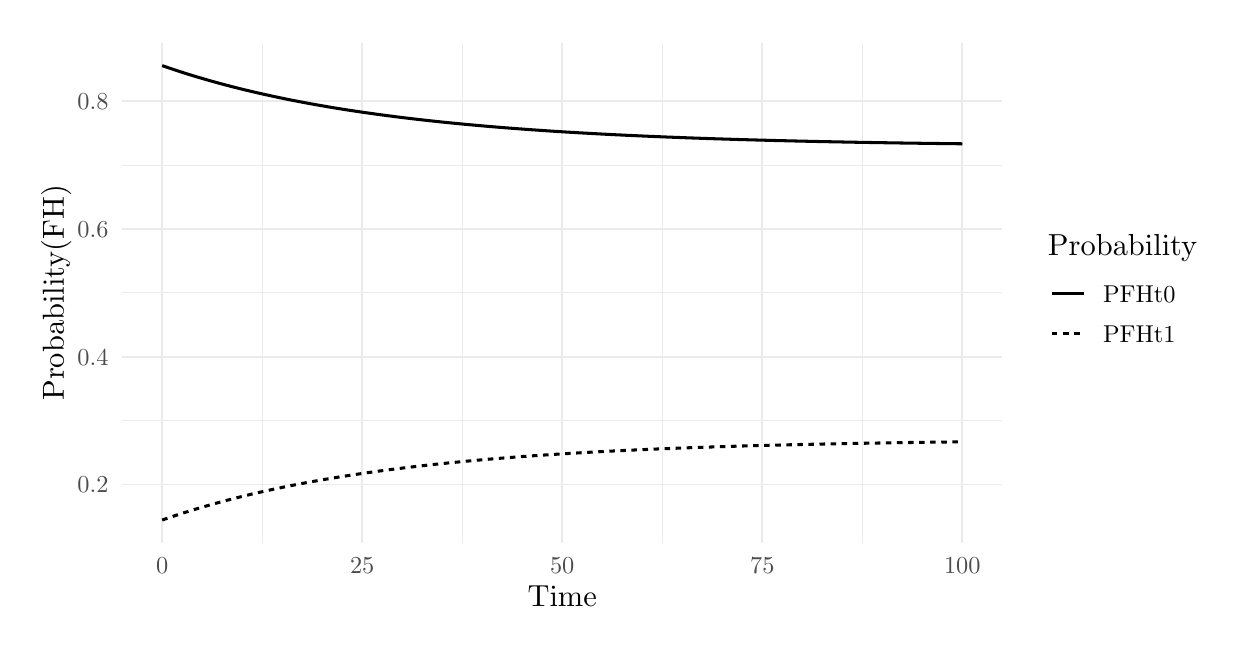
\begin{tikzpicture}[x=1pt,y=1pt]
\definecolor{fillColor}{RGB}{255,255,255}
\path[use as bounding box,fill=fillColor,fill opacity=0.00] (0,0) rectangle (433.62,216.81);
\begin{scope}
\path[clip] ( 34.16, 30.69) rectangle (352.17,211.31);
\definecolor{drawColor}{gray}{0.92}

\path[draw=drawColor,line width= 0.3pt,line join=round] ( 34.16, 74.85) --
    (352.17, 74.85);

\path[draw=drawColor,line width= 0.3pt,line join=round] ( 34.16,121.00) --
    (352.17,121.00);

\path[draw=drawColor,line width= 0.3pt,line join=round] ( 34.16,167.15) --
    (352.17,167.15);

\path[draw=drawColor,line width= 0.3pt,line join=round] ( 84.75, 30.69) --
    ( 84.75,211.31);

\path[draw=drawColor,line width= 0.3pt,line join=round] (157.03, 30.69) --
    (157.03,211.31);

\path[draw=drawColor,line width= 0.3pt,line join=round] (229.30, 30.69) --
    (229.30,211.31);

\path[draw=drawColor,line width= 0.3pt,line join=round] (301.58, 30.69) --
    (301.58,211.31);

\path[draw=drawColor,line width= 0.6pt,line join=round] ( 34.16, 51.77) --
    (352.17, 51.77);

\path[draw=drawColor,line width= 0.6pt,line join=round] ( 34.16, 97.92) --
    (352.17, 97.92);

\path[draw=drawColor,line width= 0.6pt,line join=round] ( 34.16,144.07) --
    (352.17,144.07);

\path[draw=drawColor,line width= 0.6pt,line join=round] ( 34.16,190.23) --
    (352.17,190.23);

\path[draw=drawColor,line width= 0.6pt,line join=round] ( 48.61, 30.69) --
    ( 48.61,211.31);

\path[draw=drawColor,line width= 0.6pt,line join=round] (120.89, 30.69) --
    (120.89,211.31);

\path[draw=drawColor,line width= 0.6pt,line join=round] (193.16, 30.69) --
    (193.16,211.31);

\path[draw=drawColor,line width= 0.6pt,line join=round] (265.44, 30.69) --
    (265.44,211.31);

\path[draw=drawColor,line width= 0.6pt,line join=round] (337.72, 30.69) --
    (337.72,211.31);
\definecolor{drawColor}{RGB}{0,0,0}

\path[draw=drawColor,line width= 1.1pt,line join=round] ( 48.61,203.10) --
    ( 51.50,202.10) --
    ( 54.39,201.14) --
    ( 57.28,200.21) --
    ( 60.18,199.32) --
    ( 63.07,198.46) --
    ( 65.96,197.62) --
    ( 68.85,196.82) --
    ( 71.74,196.04) --
    ( 74.63,195.29) --
    ( 77.52,194.57) --
    ( 80.41,193.87) --
    ( 83.30,193.20) --
    ( 86.20,192.55) --
    ( 89.09,191.92) --
    ( 91.98,191.31) --
    ( 94.87,190.72) --
    ( 97.76,190.16) --
    (100.65,189.61) --
    (103.54,189.08) --
    (106.43,188.57) --
    (109.32,188.08) --
    (112.21,187.60) --
    (115.11,187.14) --
    (118.00,186.70) --
    (120.89,186.27) --
    (123.78,185.86) --
    (126.67,185.46) --
    (129.56,185.07) --
    (132.45,184.70) --
    (135.34,184.33) --
    (138.23,183.99) --
    (141.13,183.65) --
    (144.02,183.32) --
    (146.91,183.01) --
    (149.80,182.70) --
    (152.69,182.41) --
    (155.58,182.13) --
    (158.47,181.85) --
    (161.36,181.59) --
    (164.25,181.33) --
    (167.14,181.08) --
    (170.04,180.84) --
    (172.93,180.61) --
    (175.82,180.39) --
    (178.71,180.17) --
    (181.60,179.96) --
    (184.49,179.76) --
    (187.38,179.56) --
    (190.27,179.37) --
    (193.16,179.19) --
    (196.05,179.01) --
    (198.95,178.84) --
    (201.84,178.68) --
    (204.73,178.52) --
    (207.62,178.36) --
    (210.51,178.21) --
    (213.40,178.07) --
    (216.29,177.93) --
    (219.18,177.80) --
    (222.07,177.67) --
    (224.97,177.54) --
    (227.86,177.42) --
    (230.75,177.30) --
    (233.64,177.19) --
    (236.53,177.08) --
    (239.42,176.97) --
    (242.31,176.87) --
    (245.20,176.77) --
    (248.09,176.67) --
    (250.98,176.58) --
    (253.88,176.49) --
    (256.77,176.40) --
    (259.66,176.32) --
    (262.55,176.24) --
    (265.44,176.16) --
    (268.33,176.08) --
    (271.22,176.01) --
    (274.11,175.94) --
    (277.00,175.87) --
    (279.90,175.80) --
    (282.79,175.74) --
    (285.68,175.67) --
    (288.57,175.61) --
    (291.46,175.56) --
    (294.35,175.50) --
    (297.24,175.44) --
    (300.13,175.39) --
    (303.02,175.34) --
    (305.91,175.29) --
    (308.81,175.24) --
    (311.70,175.20) --
    (314.59,175.15) --
    (317.48,175.11) --
    (320.37,175.07) --
    (323.26,175.03) --
    (326.15,174.99) --
    (329.04,174.95) --
    (331.93,174.92) --
    (334.83,174.88) --
    (337.72,174.85);

\path[draw=drawColor,line width= 1.1pt,dash pattern=on 2pt off 2pt ,line join=round] ( 48.61, 38.90) --
    ( 51.50, 39.89) --
    ( 54.39, 40.85) --
    ( 57.28, 41.78) --
    ( 60.18, 42.68) --
    ( 63.07, 43.54) --
    ( 65.96, 44.37) --
    ( 68.85, 45.18) --
    ( 71.74, 45.95) --
    ( 74.63, 46.70) --
    ( 77.52, 47.43) --
    ( 80.41, 48.13) --
    ( 83.30, 48.80) --
    ( 86.20, 49.45) --
    ( 89.09, 50.08) --
    ( 91.98, 50.69) --
    ( 94.87, 51.27) --
    ( 97.76, 51.84) --
    (100.65, 52.39) --
    (103.54, 52.91) --
    (106.43, 53.42) --
    (109.32, 53.92) --
    (112.21, 54.39) --
    (115.11, 54.85) --
    (118.00, 55.30) --
    (120.89, 55.72) --
    (123.78, 56.14) --
    (126.67, 56.54) --
    (129.56, 56.93) --
    (132.45, 57.30) --
    (135.34, 57.66) --
    (138.23, 58.01) --
    (141.13, 58.35) --
    (144.02, 58.67) --
    (146.91, 58.99) --
    (149.80, 59.29) --
    (152.69, 59.59) --
    (155.58, 59.87) --
    (158.47, 60.15) --
    (161.36, 60.41) --
    (164.25, 60.67) --
    (167.14, 60.92) --
    (170.04, 61.15) --
    (172.93, 61.39) --
    (175.82, 61.61) --
    (178.71, 61.83) --
    (181.60, 62.04) --
    (184.49, 62.24) --
    (187.38, 62.43) --
    (190.27, 62.62) --
    (193.16, 62.81) --
    (196.05, 62.98) --
    (198.95, 63.15) --
    (201.84, 63.32) --
    (204.73, 63.48) --
    (207.62, 63.63) --
    (210.51, 63.78) --
    (213.40, 63.93) --
    (216.29, 64.06) --
    (219.18, 64.20) --
    (222.07, 64.33) --
    (224.97, 64.46) --
    (227.86, 64.58) --
    (230.75, 64.70) --
    (233.64, 64.81) --
    (236.53, 64.92) --
    (239.42, 65.03) --
    (242.31, 65.13) --
    (245.20, 65.23) --
    (248.09, 65.32) --
    (250.98, 65.42) --
    (253.88, 65.51) --
    (256.77, 65.60) --
    (259.66, 65.68) --
    (262.55, 65.76) --
    (265.44, 65.84) --
    (268.33, 65.92) --
    (271.22, 65.99) --
    (274.11, 66.06) --
    (277.00, 66.13) --
    (279.90, 66.20) --
    (282.79, 66.26) --
    (285.68, 66.32) --
    (288.57, 66.38) --
    (291.46, 66.44) --
    (294.35, 66.50) --
    (297.24, 66.55) --
    (300.13, 66.60) --
    (303.02, 66.65) --
    (305.91, 66.70) --
    (308.81, 66.75) --
    (311.70, 66.80) --
    (314.59, 66.84) --
    (317.48, 66.89) --
    (320.37, 66.93) --
    (323.26, 66.97) --
    (326.15, 67.01) --
    (329.04, 67.04) --
    (331.93, 67.08) --
    (334.83, 67.12) --
    (337.72, 67.15);
\end{scope}
\begin{scope}
\path[clip] (  0.00,  0.00) rectangle (433.62,216.81);
\definecolor{drawColor}{gray}{0.30}

\node[text=drawColor,anchor=base east,inner sep=0pt, outer sep=0pt, scale=  0.88] at ( 29.21, 48.74) {0.2};

\node[text=drawColor,anchor=base east,inner sep=0pt, outer sep=0pt, scale=  0.88] at ( 29.21, 94.89) {0.4};

\node[text=drawColor,anchor=base east,inner sep=0pt, outer sep=0pt, scale=  0.88] at ( 29.21,141.04) {0.6};

\node[text=drawColor,anchor=base east,inner sep=0pt, outer sep=0pt, scale=  0.88] at ( 29.21,187.20) {0.8};
\end{scope}
\begin{scope}
\path[clip] (  0.00,  0.00) rectangle (433.62,216.81);
\definecolor{drawColor}{gray}{0.30}

\node[text=drawColor,anchor=base,inner sep=0pt, outer sep=0pt, scale=  0.88] at ( 48.61, 19.68) {0};

\node[text=drawColor,anchor=base,inner sep=0pt, outer sep=0pt, scale=  0.88] at (120.89, 19.68) {25};

\node[text=drawColor,anchor=base,inner sep=0pt, outer sep=0pt, scale=  0.88] at (193.16, 19.68) {50};

\node[text=drawColor,anchor=base,inner sep=0pt, outer sep=0pt, scale=  0.88] at (265.44, 19.68) {75};

\node[text=drawColor,anchor=base,inner sep=0pt, outer sep=0pt, scale=  0.88] at (337.72, 19.68) {100};
\end{scope}
\begin{scope}
\path[clip] (  0.00,  0.00) rectangle (433.62,216.81);
\definecolor{drawColor}{RGB}{0,0,0}

\node[text=drawColor,anchor=base,inner sep=0pt, outer sep=0pt, scale=  1.10] at (193.16,  7.64) {Time};
\end{scope}
\begin{scope}
\path[clip] (  0.00,  0.00) rectangle (433.62,216.81);
\definecolor{drawColor}{RGB}{0,0,0}

\node[text=drawColor,rotate= 90.00,anchor=base,inner sep=0pt, outer sep=0pt, scale=  1.10] at ( 13.08,121.00) {Probability(FH)};
\end{scope}
\begin{scope}
\path[clip] (  0.00,  0.00) rectangle (433.62,216.81);
\definecolor{drawColor}{RGB}{0,0,0}

\node[text=drawColor,anchor=base west,inner sep=0pt, outer sep=0pt, scale=  1.10] at (368.67,134.41) {Probability};
\end{scope}
\begin{scope}
\path[clip] (  0.00,  0.00) rectangle (433.62,216.81);
\definecolor{drawColor}{RGB}{0,0,0}

\path[draw=drawColor,line width= 1.1pt,line join=round] (370.12,120.62) -- (381.68,120.62);
\end{scope}
\begin{scope}
\path[clip] (  0.00,  0.00) rectangle (433.62,216.81);
\definecolor{drawColor}{RGB}{0,0,0}

\path[draw=drawColor,line width= 1.1pt,dash pattern=on 2pt off 2pt ,line join=round] (370.12,106.16) -- (381.68,106.16);
\end{scope}
\begin{scope}
\path[clip] (  0.00,  0.00) rectangle (433.62,216.81);
\definecolor{drawColor}{RGB}{0,0,0}

\node[text=drawColor,anchor=base west,inner sep=0pt, outer sep=0pt, scale=  0.88] at (388.63,117.59) {PFHt0};
\end{scope}
\begin{scope}
\path[clip] (  0.00,  0.00) rectangle (433.62,216.81);
\definecolor{drawColor}{RGB}{0,0,0}

\node[text=drawColor,anchor=base west,inner sep=0pt, outer sep=0pt, scale=  0.88] at (388.63,103.13) {PFHt1};
\end{scope}
\end{tikzpicture}
    \caption{Probability of FH = 0 (PFHt0) vs Probability of FH = 1 (PFHt1)}
    \label{fig:disease 0}
\end{figure}
The difference between the two indicators can assume the values: $(FH(t) - R) \in \left\{-1, 0, 1\right\}$. We would like to be as close as possible to the scenario with no difference between the indicators. Importantly, $R$ is fixed while $FH(t)$ depends on $t$. 

% We compute the probabilities of the agreement for low and high-risk group membership. The conditional probability of agreement in the low-risk group over the whole $\mathbb{R}^+$ time axis is:

We now compute the probabilities of the agreement for low and high-risk group membership. For the survival case we recall that the hazard function in the low (high) risk group is $\lambda_0(t)$ ($\lambda_1(t)=\alpha\cdot\lambda_0(t)$). keeping in mind that  $\lambda(t\mid R=0)=\lambda_0=\lambda$ and $\lambda(t\mid R=1)=\lambda_1(t)=\beta\lambda_0(t)=\beta\lambda$. But this does not hold in the disease development case. The probability of agreement in the low-risk group over the whole $\mathbb{R}^+$ time axis is: 
\begin{align*}
    %\label{prob_0}
    P(FH_i(b_i+t) = R_i\mid R_i=0) &=\int_0^{\infty}P(FH_i(b_i+t)=0)f_{0}(t)\text{d}t \nonumber \\
    &=\int_0^{\infty}\left(p+(1-p)\text{e}^{-\lambda^*(t+60)}\right)\left(p+(1-p)\text{e}^{-\lambda^*(t+30)}\right)\cdot\\ 
    &\cdot\left(p+(1-p)\text{e}^{-\lambda^*t}\right)(1-p)\lambda^* e^{-\lambda^* t}\text{d}t
\end{align*}
Similarly, we compute the probability of agreement for the high-risk group:
    \begin{align*}
    %\label{prob_1}
    &P(FH_i(b_i+t) = R_i\mid R_i=1) =\int_0^{\infty}P(FH_i(b_i+t)=1)f_{1}(t)\text{d}t \\
    &\quad=\int_0^{\infty}(1 - P(FH_i(b_i+t)=0))f_1(t,\lambda^*)\text{d}t \nonumber \\
    &\quad=\int_0^{\infty}f_1(t,\lambda^*) - P(FH_i(b_i+t)=0)f_1(t,\lambda^*)\text{d}t \nonumber \\
    &\quad=\int_0^{\infty}f_1(t,\lambda^*)\text{d}t - \int_0^{\infty}P(FH_i(b_i+t)=0)f_1(t,\lambda^*)\text{d}t  \\
    &\quad=1 - \int_0^{\infty}P(FH_i(b_i+t)=0)f_1(t,\lambda^*)\text{d}t\nonumber \\
    &\quad=1 - \int_0^{\infty}P(FH_i(b_i+t)=0)(1-\widetilde{p})\left(\frac{f^*(t)e^{\alpha}}{1-\widetilde{p}}\right)(p+(1-p)\widetilde{S}(t))^{e^\alpha-1}\text{d}t \nonumber
\end{align*} 
One would like both probabilities to be large. For the cure rate case, the conditional probability of agreement in the low-risk group over the whole $\mathbb{R}^+$ time axis is: 
\begin{align*}
    % \label{formula:1_2}
    P(FH_i(b_i+t) = R_i\mid R_i=0) &=\int_0^{\infty}P(FH_i(b_i+t)=0)f_0(t)\text{d}t 
\end{align*} Easily, we obtain the conditional probability of agreement for the high-risk group:
\begin{align*}
    % \label{formula:1_3}
    P(F H_i(b_i+t) = R_i\mid R_i=1)  &=\int_0^{\infty}P(F H_i(b_i+t)=1)f_1(t)\text{d}t
\end{align*} 
We can also analyse the misclassification probabilities (note that we implicitly assume that the proportion of high-risk families $P(R=1)=h$ is constant over time).
For the cure rate case the conditional correct classification probabilities are: \begin{align*}
    % \label{probs_final}
    &P(FH_i(t)=0\mid R_i=0)=S_0(t+60)S_0(t+30)S_0(t) \\
    &\qquad\qquad\qquad=(p+(1-p)\widetilde{S}(t+60)) (p+(1-p)\widetilde{S}(t+30)) (p+(1-p)\widetilde{S}(t)) \\
    &\qquad\qquad\qquad=(p+(1-p)e^{-\lambda^*(t+60)}) (p+(1-p)e^{-\lambda^*(t+30)}) (p+(1-p)e^{-\lambda^*(t)}) \\
    &P(FH_i(t)=0\mid R_i=1) = S_1(t+60)S_1(t+30)S_1(t) = (S_0(t+60)S_0(t+30)S_0(t))^{e^\alpha} \\
    &\qquad\qquad\qquad=((p+(1-p)e^{-\lambda^*(t+60)}) (p+(1-p)e^{-\lambda^*(t+30)}) (p+(1-p)e^{-\lambda^*(t)}))^{e^\alpha}
\end{align*} 
Clearly, \begin{align*}
    &S_0(t) = p+(1-p)e^{-\lambda^*(t)} \\
    &S_1(t) = (p+(1-p)e^{-\lambda^*(t)})^{e^\alpha}  \\
    &P(FH_i(t)=1\mid R_i=0) = 1 - S_0(t+60)S_0(t+30)S_0(t) \\
    &P(FH_i(t)=1\mid R_i=1) = 1 - S_1(t+60)S_1(t+30)S_1(t)
\end{align*} 
A graphical visualization of these probabilities is illustrated in Figure \ref{fig:disease 1}. 
\begin{figure}[ht]
    \centering
    % \includegraphics{plots/plot_1_disease.png}
    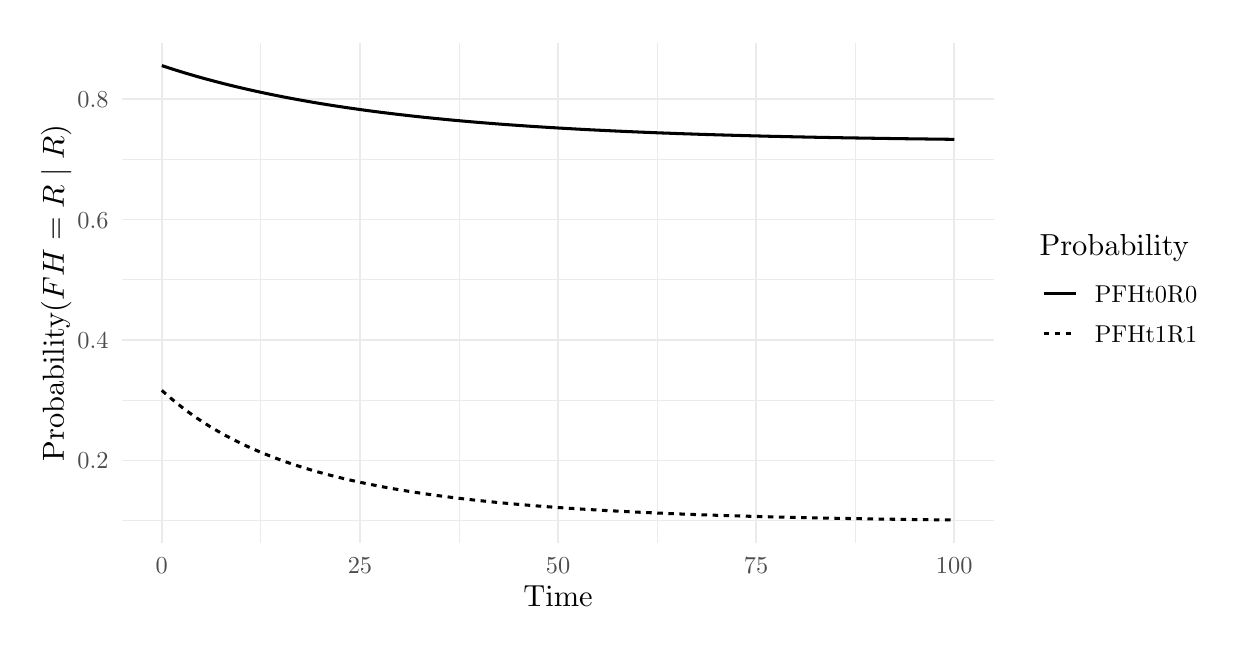
\begin{tikzpicture}[x=1pt,y=1pt]
\definecolor{fillColor}{RGB}{255,255,255}
\path[use as bounding box,fill=fillColor,fill opacity=0.00] (0,0) rectangle (433.62,216.81);
\begin{scope}
\path[clip] ( 34.16, 30.69) rectangle (349.14,211.31);
\definecolor{drawColor}{gray}{0.92}

\path[draw=drawColor,line width= 0.3pt,line join=round] ( 34.16, 38.66) --
    (349.14, 38.66);

\path[draw=drawColor,line width= 0.3pt,line join=round] ( 34.16, 82.17) --
    (349.14, 82.17);

\path[draw=drawColor,line width= 0.3pt,line join=round] ( 34.16,125.69) --
    (349.14,125.69);

\path[draw=drawColor,line width= 0.3pt,line join=round] ( 34.16,169.20) --
    (349.14,169.20);

\path[draw=drawColor,line width= 0.3pt,line join=round] ( 84.27, 30.69) --
    ( 84.27,211.31);

\path[draw=drawColor,line width= 0.3pt,line join=round] (155.86, 30.69) --
    (155.86,211.31);

\path[draw=drawColor,line width= 0.3pt,line join=round] (227.44, 30.69) --
    (227.44,211.31);

\path[draw=drawColor,line width= 0.3pt,line join=round] (299.03, 30.69) --
    (299.03,211.31);

\path[draw=drawColor,line width= 0.6pt,line join=round] ( 34.16, 60.41) --
    (349.14, 60.41);

\path[draw=drawColor,line width= 0.6pt,line join=round] ( 34.16,103.93) --
    (349.14,103.93);

\path[draw=drawColor,line width= 0.6pt,line join=round] ( 34.16,147.45) --
    (349.14,147.45);

\path[draw=drawColor,line width= 0.6pt,line join=round] ( 34.16,190.96) --
    (349.14,190.96);

\path[draw=drawColor,line width= 0.6pt,line join=round] ( 48.47, 30.69) --
    ( 48.47,211.31);

\path[draw=drawColor,line width= 0.6pt,line join=round] (120.06, 30.69) --
    (120.06,211.31);

\path[draw=drawColor,line width= 0.6pt,line join=round] (191.65, 30.69) --
    (191.65,211.31);

\path[draw=drawColor,line width= 0.6pt,line join=round] (263.24, 30.69) --
    (263.24,211.31);

\path[draw=drawColor,line width= 0.6pt,line join=round] (334.82, 30.69) --
    (334.82,211.31);
\definecolor{drawColor}{RGB}{0,0,0}

\path[draw=drawColor,line width= 1.1pt,line join=round] ( 48.47,203.10) --
    ( 51.34,202.16) --
    ( 54.20,201.25) --
    ( 57.06,200.38) --
    ( 59.93,199.54) --
    ( 62.79,198.72) --
    ( 65.65,197.94) --
    ( 68.52,197.18) --
    ( 71.38,196.45) --
    ( 74.25,195.74) --
    ( 77.11,195.06) --
    ( 79.97,194.40) --
    ( 82.84,193.76) --
    ( 85.70,193.15) --
    ( 88.56,192.56) --
    ( 91.43,191.98) --
    ( 94.29,191.43) --
    ( 97.15,190.90) --
    (100.02,190.38) --
    (102.88,189.88) --
    (105.74,189.40) --
    (108.61,188.94) --
    (111.47,188.49) --
    (114.33,188.06) --
    (117.20,187.64) --
    (120.06,187.23) --
    (122.92,186.84) --
    (125.79,186.46) --
    (128.65,186.10) --
    (131.52,185.75) --
    (134.38,185.41) --
    (137.24,185.08) --
    (140.11,184.76) --
    (142.97,184.45) --
    (145.83,184.16) --
    (148.70,183.87) --
    (151.56,183.59) --
    (154.42,183.32) --
    (157.29,183.06) --
    (160.15,182.81) --
    (163.01,182.57) --
    (165.88,182.34) --
    (168.74,182.11) --
    (171.60,181.89) --
    (174.47,181.68) --
    (177.33,181.48) --
    (180.19,181.28) --
    (183.06,181.09) --
    (185.92,180.91) --
    (188.79,180.73) --
    (191.65,180.56) --
    (194.51,180.39) --
    (197.38,180.23) --
    (200.24,180.07) --
    (203.10,179.92) --
    (205.97,179.78) --
    (208.83,179.64) --
    (211.69,179.50) --
    (214.56,179.37) --
    (217.42,179.24) --
    (220.28,179.12) --
    (223.15,179.00) --
    (226.01,178.88) --
    (228.87,178.77) --
    (231.74,178.67) --
    (234.60,178.56) --
    (237.46,178.46) --
    (240.33,178.37) --
    (243.19,178.27) --
    (246.06,178.18) --
    (248.92,178.09) --
    (251.78,178.01) --
    (254.65,177.93) --
    (257.51,177.85) --
    (260.37,177.77) --
    (263.24,177.70) --
    (266.10,177.62) --
    (268.96,177.55) --
    (271.83,177.49) --
    (274.69,177.42) --
    (277.55,177.36) --
    (280.42,177.30) --
    (283.28,177.24) --
    (286.14,177.18) --
    (289.01,177.13) --
    (291.87,177.08) --
    (294.73,177.02) --
    (297.60,176.97) --
    (300.46,176.93) --
    (303.33,176.88) --
    (306.19,176.84) --
    (309.05,176.79) --
    (311.92,176.75) --
    (314.78,176.71) --
    (317.64,176.67) --
    (320.51,176.63) --
    (323.37,176.60) --
    (326.23,176.56) --
    (329.10,176.53) --
    (331.96,176.49) --
    (334.82,176.46);

\path[draw=drawColor,line width= 1.1pt,dash pattern=on 2pt off 2pt ,line join=round] ( 48.47, 85.74) --
    ( 51.34, 83.22) --
    ( 54.20, 80.86) --
    ( 57.06, 78.65) --
    ( 59.93, 76.58) --
    ( 62.79, 74.64) --
    ( 65.65, 72.82) --
    ( 68.52, 71.11) --
    ( 71.38, 69.51) --
    ( 74.25, 68.00) --
    ( 77.11, 66.57) --
    ( 79.97, 65.23) --
    ( 82.84, 63.97) --
    ( 85.70, 62.78) --
    ( 88.56, 61.65) --
    ( 91.43, 60.58) --
    ( 94.29, 59.57) --
    ( 97.15, 58.62) --
    (100.02, 57.71) --
    (102.88, 56.85) --
    (105.74, 56.04) --
    (108.61, 55.27) --
    (111.47, 54.54) --
    (114.33, 53.84) --
    (117.20, 53.18) --
    (120.06, 52.55) --
    (122.92, 51.95) --
    (125.79, 51.38) --
    (128.65, 50.83) --
    (131.52, 50.31) --
    (134.38, 49.82) --
    (137.24, 49.35) --
    (140.11, 48.90) --
    (142.97, 48.46) --
    (145.83, 48.05) --
    (148.70, 47.66) --
    (151.56, 47.29) --
    (154.42, 46.93) --
    (157.29, 46.58) --
    (160.15, 46.25) --
    (163.01, 45.94) --
    (165.88, 45.64) --
    (168.74, 45.35) --
    (171.60, 45.07) --
    (174.47, 44.81) --
    (177.33, 44.55) --
    (180.19, 44.31) --
    (183.06, 44.07) --
    (185.92, 43.85) --
    (188.79, 43.63) --
    (191.65, 43.43) --
    (194.51, 43.23) --
    (197.38, 43.04) --
    (200.24, 42.85) --
    (203.10, 42.68) --
    (205.97, 42.51) --
    (208.83, 42.34) --
    (211.69, 42.19) --
    (214.56, 42.04) --
    (217.42, 41.89) --
    (220.28, 41.75) --
    (223.15, 41.62) --
    (226.01, 41.49) --
    (228.87, 41.37) --
    (231.74, 41.25) --
    (234.60, 41.13) --
    (237.46, 41.02) --
    (240.33, 40.91) --
    (243.19, 40.81) --
    (246.06, 40.71) --
    (248.92, 40.61) --
    (251.78, 40.52) --
    (254.65, 40.43) --
    (257.51, 40.35) --
    (260.37, 40.27) --
    (263.24, 40.19) --
    (266.10, 40.11) --
    (268.96, 40.04) --
    (271.83, 39.96) --
    (274.69, 39.90) --
    (277.55, 39.83) --
    (280.42, 39.77) --
    (283.28, 39.70) --
    (286.14, 39.64) --
    (289.01, 39.59) --
    (291.87, 39.53) --
    (294.73, 39.48) --
    (297.60, 39.43) --
    (300.46, 39.38) --
    (303.33, 39.33) --
    (306.19, 39.28) --
    (309.05, 39.24) --
    (311.92, 39.19) --
    (314.78, 39.15) --
    (317.64, 39.11) --
    (320.51, 39.07) --
    (323.37, 39.03) --
    (326.23, 39.00) --
    (329.10, 38.96) --
    (331.96, 38.93) --
    (334.82, 38.90);
\end{scope}
\begin{scope}
\path[clip] (  0.00,  0.00) rectangle (433.62,216.81);
\definecolor{drawColor}{gray}{0.30}

\node[text=drawColor,anchor=base east,inner sep=0pt, outer sep=0pt, scale=  0.88] at ( 29.21, 57.38) {0.2};

\node[text=drawColor,anchor=base east,inner sep=0pt, outer sep=0pt, scale=  0.88] at ( 29.21,100.90) {0.4};

\node[text=drawColor,anchor=base east,inner sep=0pt, outer sep=0pt, scale=  0.88] at ( 29.21,144.42) {0.6};

\node[text=drawColor,anchor=base east,inner sep=0pt, outer sep=0pt, scale=  0.88] at ( 29.21,187.93) {0.8};
\end{scope}
\begin{scope}
\path[clip] (  0.00,  0.00) rectangle (433.62,216.81);
\definecolor{drawColor}{gray}{0.30}

\node[text=drawColor,anchor=base,inner sep=0pt, outer sep=0pt, scale=  0.88] at ( 48.47, 19.68) {0};

\node[text=drawColor,anchor=base,inner sep=0pt, outer sep=0pt, scale=  0.88] at (120.06, 19.68) {25};

\node[text=drawColor,anchor=base,inner sep=0pt, outer sep=0pt, scale=  0.88] at (191.65, 19.68) {50};

\node[text=drawColor,anchor=base,inner sep=0pt, outer sep=0pt, scale=  0.88] at (263.24, 19.68) {75};

\node[text=drawColor,anchor=base,inner sep=0pt, outer sep=0pt, scale=  0.88] at (334.82, 19.68) {100};
\end{scope}
\begin{scope}
\path[clip] (  0.00,  0.00) rectangle (433.62,216.81);
\definecolor{drawColor}{RGB}{0,0,0}

\node[text=drawColor,anchor=base,inner sep=0pt, outer sep=0pt, scale=  1.10] at (191.65,  7.64) {Time};
\end{scope}
\begin{scope}
\path[clip] (  0.00,  0.00) rectangle (433.62,216.81);
\definecolor{drawColor}{RGB}{0,0,0}

\node[text=drawColor,rotate= 90.00,anchor=base,inner sep=0pt, outer sep=0pt, scale=  1.10] at ( 13.08,121.00) {Probability($FH = R\mid R$)};
\end{scope}
\begin{scope}
\path[clip] (  0.00,  0.00) rectangle (433.62,216.81);
\definecolor{drawColor}{RGB}{0,0,0}

\node[text=drawColor,anchor=base west,inner sep=0pt, outer sep=0pt, scale=  1.10] at (365.64,134.41) {Probability};
\end{scope}
\begin{scope}
\path[clip] (  0.00,  0.00) rectangle (433.62,216.81);
\definecolor{drawColor}{RGB}{0,0,0}

\path[draw=drawColor,line width= 1.1pt,line join=round] (367.09,120.62) -- (378.65,120.62);
\end{scope}
\begin{scope}
\path[clip] (  0.00,  0.00) rectangle (433.62,216.81);
\definecolor{drawColor}{RGB}{0,0,0}

\path[draw=drawColor,line width= 1.1pt,dash pattern=on 2pt off 2pt ,line join=round] (367.09,106.16) -- (378.65,106.16);
\end{scope}
\begin{scope}
\path[clip] (  0.00,  0.00) rectangle (433.62,216.81);
\definecolor{drawColor}{RGB}{0,0,0}

\node[text=drawColor,anchor=base west,inner sep=0pt, outer sep=0pt, scale=  0.88] at (385.60,117.59) {PFHt0R0};
\end{scope}
\begin{scope}
\path[clip] (  0.00,  0.00) rectangle (433.62,216.81);
\definecolor{drawColor}{RGB}{0,0,0}

\node[text=drawColor,anchor=base west,inner sep=0pt, outer sep=0pt, scale=  0.88] at (385.60,103.13) {PFHt1R1};
\end{scope}
\end{tikzpicture}
    \caption{Probability of $FH = 0$ conditional to $R = 0$ (PFHt0R0) vs. Probability of $(FH = 1$ conditional to $R=1$ (PFHt1R1)}
    \label{fig:disease 1}
\end{figure}
We also compute the inverse probabilities of correct classification only for the survival case, i.e.: (i) $P(R_i=0\mid FH_i(t)=0)$ and (ii) $P(R_i=1\mid FH_i(t)=1)$. These are: \begin{align*}
    &(i) \ P(R_i = 0\mid FH_i(t)=0) = \frac{P(FH_i(t)=0\mid R_i=0)P(R_i=0)}{P(FH_i(t)=0)} \\
    &= \frac{P(FH_i(t)=0\mid R_i=0)(1-h)}{P(FH_i(t)=0\mid R_i=0)(1-h) +P(FH_i(t)=0\mid R_i=1)h} \\
    &= \frac{\overbrace{((p+(1-p)e^{-\lambda^*(t+60)}) (p+(1-p)e^{-\lambda^*(t+30)}) (p+(1-p)e^{-\lambda^*(t)}))}^{(*)}(1-h)}{(*)(1-h)+\left(((p+(1-p)e^{-\lambda^*(t+60)}) (p+(1-p)e^{-\lambda^*(t+30)}) (p+(1-p)e^{-\lambda^*(t)}))^{e^\alpha} \right)h}
\end{align*} and \begin{align*}
    &(ii) \ P(R_i = 1\mid FH_i(t)=1) = \frac{P(FH_i(t)=1\mid R_i=1)P(R_i=1)}{P(FH_i(t)=1)}  \\
    &= \frac{P(FH_i(t)=1\mid R_i=1)h}{P(FH_i(t)=1\mid R_i=1)h +P(FH_i(t)=1\mid R_i=0)(1-h) } \\
    &=\frac{\overbrace{(1-((p+(1-p)e^{-\lambda^*(t+60)}) (p+(1-p)e^{-\lambda^*(t+30)}) (p+(1-p)e^{-\lambda^*(t)}))^{e^\alpha})}^{(*)}h}{(*)h+\left(1-(p+(1-p)e^{-\lambda^*(t+60)}) (p+(1-p)e^{-\lambda^*(t+30)}) (p+(1-p)e^{-\lambda^*(t)})\right)(1-h)}
\end{align*}
With these probabilities, we describe the distribution of the measurement error when using the observed $FH(t)$ instead of $R$ in the observed data model. A graphical representation of the trend of these probabilities for the fixed values $\lambda=1/90$, $\alpha=2$, $h=0.7$ is illustrated in figure \ref{fig:disease 2}. \begin{figure}[ht]
    \centering
    % \includegraphics{plots/plot_2_disease.png}
    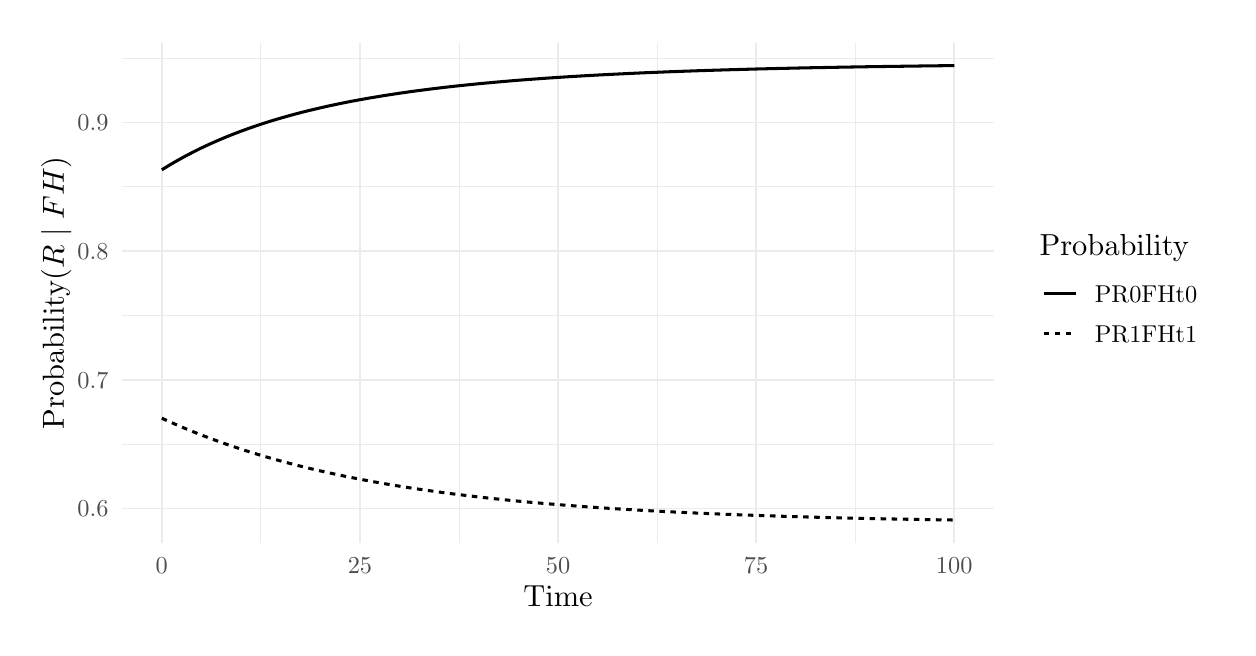
\begin{tikzpicture}[x=1pt,y=1pt]
\definecolor{fillColor}{RGB}{255,255,255}
\path[use as bounding box,fill=fillColor,fill opacity=0.00] (0,0) rectangle (433.62,216.81);
\begin{scope}
\path[clip] ( 34.16, 30.69) rectangle (349.14,211.31);
\definecolor{drawColor}{gray}{0.92}

\path[draw=drawColor,line width= 0.3pt,line join=round] ( 34.16, 66.34) --
    (349.14, 66.34);

\path[draw=drawColor,line width= 0.3pt,line join=round] ( 34.16,112.82) --
    (349.14,112.82);

\path[draw=drawColor,line width= 0.3pt,line join=round] ( 34.16,159.31) --
    (349.14,159.31);

\path[draw=drawColor,line width= 0.3pt,line join=round] ( 34.16,205.79) --
    (349.14,205.79);

\path[draw=drawColor,line width= 0.3pt,line join=round] ( 84.27, 30.69) --
    ( 84.27,211.31);

\path[draw=drawColor,line width= 0.3pt,line join=round] (155.86, 30.69) --
    (155.86,211.31);

\path[draw=drawColor,line width= 0.3pt,line join=round] (227.44, 30.69) --
    (227.44,211.31);

\path[draw=drawColor,line width= 0.3pt,line join=round] (299.03, 30.69) --
    (299.03,211.31);

\path[draw=drawColor,line width= 0.6pt,line join=round] ( 34.16, 43.10) --
    (349.14, 43.10);

\path[draw=drawColor,line width= 0.6pt,line join=round] ( 34.16, 89.58) --
    (349.14, 89.58);

\path[draw=drawColor,line width= 0.6pt,line join=round] ( 34.16,136.07) --
    (349.14,136.07);

\path[draw=drawColor,line width= 0.6pt,line join=round] ( 34.16,182.55) --
    (349.14,182.55);

\path[draw=drawColor,line width= 0.6pt,line join=round] ( 48.47, 30.69) --
    ( 48.47,211.31);

\path[draw=drawColor,line width= 0.6pt,line join=round] (120.06, 30.69) --
    (120.06,211.31);

\path[draw=drawColor,line width= 0.6pt,line join=round] (191.65, 30.69) --
    (191.65,211.31);

\path[draw=drawColor,line width= 0.6pt,line join=round] (263.24, 30.69) --
    (263.24,211.31);

\path[draw=drawColor,line width= 0.6pt,line join=round] (334.82, 30.69) --
    (334.82,211.31);
\definecolor{drawColor}{RGB}{0,0,0}

\path[draw=drawColor,line width= 1.1pt,line join=round] ( 48.47,165.45) --
    ( 51.34,167.21) --
    ( 54.20,168.87) --
    ( 57.06,170.44) --
    ( 59.93,171.93) --
    ( 62.79,173.35) --
    ( 65.65,174.69) --
    ( 68.52,175.96) --
    ( 71.38,177.17) --
    ( 74.25,178.32) --
    ( 77.11,179.41) --
    ( 79.97,180.45) --
    ( 82.84,181.44) --
    ( 85.70,182.38) --
    ( 88.56,183.28) --
    ( 91.43,184.13) --
    ( 94.29,184.94) --
    ( 97.15,185.72) --
    (100.02,186.46) --
    (102.88,187.16) --
    (105.74,187.83) --
    (108.61,188.48) --
    (111.47,189.09) --
    (114.33,189.68) --
    (117.20,190.24) --
    (120.06,190.77) --
    (122.92,191.28) --
    (125.79,191.77) --
    (128.65,192.24) --
    (131.52,192.69) --
    (134.38,193.12) --
    (137.24,193.53) --
    (140.11,193.93) --
    (142.97,194.30) --
    (145.83,194.67) --
    (148.70,195.01) --
    (151.56,195.35) --
    (154.42,195.67) --
    (157.29,195.97) --
    (160.15,196.27) --
    (163.01,196.55) --
    (165.88,196.82) --
    (168.74,197.08) --
    (171.60,197.33) --
    (174.47,197.58) --
    (177.33,197.81) --
    (180.19,198.03) --
    (183.06,198.24) --
    (185.92,198.45) --
    (188.79,198.65) --
    (191.65,198.84) --
    (194.51,199.02) --
    (197.38,199.20) --
    (200.24,199.37) --
    (203.10,199.53) --
    (205.97,199.69) --
    (208.83,199.84) --
    (211.69,199.98) --
    (214.56,200.12) --
    (217.42,200.26) --
    (220.28,200.39) --
    (223.15,200.52) --
    (226.01,200.64) --
    (228.87,200.75) --
    (231.74,200.87) --
    (234.60,200.97) --
    (237.46,201.08) --
    (240.33,201.18) --
    (243.19,201.28) --
    (246.06,201.37) --
    (248.92,201.46) --
    (251.78,201.55) --
    (254.65,201.63) --
    (257.51,201.71) --
    (260.37,201.79) --
    (263.24,201.87) --
    (266.10,201.94) --
    (268.96,202.01) --
    (271.83,202.08) --
    (274.69,202.14) --
    (277.55,202.21) --
    (280.42,202.27) --
    (283.28,202.33) --
    (286.14,202.38) --
    (289.01,202.44) --
    (291.87,202.49) --
    (294.73,202.54) --
    (297.60,202.59) --
    (300.46,202.64) --
    (303.33,202.69) --
    (306.19,202.73) --
    (309.05,202.77) --
    (311.92,202.81) --
    (314.78,202.85) --
    (317.64,202.89) --
    (320.51,202.93) --
    (323.37,202.97) --
    (326.23,203.00) --
    (329.10,203.04) --
    (331.96,203.07) --
    (334.82,203.10);

\path[draw=drawColor,line width= 1.1pt,dash pattern=on 2pt off 2pt ,line join=round] ( 48.47, 75.70) --
    ( 51.34, 74.39) --
    ( 54.20, 73.13) --
    ( 57.06, 71.92) --
    ( 59.93, 70.75) --
    ( 62.79, 69.61) --
    ( 65.65, 68.52) --
    ( 68.52, 67.46) --
    ( 71.38, 66.44) --
    ( 74.25, 65.46) --
    ( 77.11, 64.51) --
    ( 79.97, 63.59) --
    ( 82.84, 62.71) --
    ( 85.70, 61.85) --
    ( 88.56, 61.03) --
    ( 91.43, 60.23) --
    ( 94.29, 59.47) --
    ( 97.15, 58.72) --
    (100.02, 58.01) --
    (102.88, 57.32) --
    (105.74, 56.65) --
    (108.61, 56.01) --
    (111.47, 55.39) --
    (114.33, 54.78) --
    (117.20, 54.21) --
    (120.06, 53.65) --
    (122.92, 53.11) --
    (125.79, 52.58) --
    (128.65, 52.08) --
    (131.52, 51.59) --
    (134.38, 51.12) --
    (137.24, 50.67) --
    (140.11, 50.23) --
    (142.97, 49.81) --
    (145.83, 49.40) --
    (148.70, 49.00) --
    (151.56, 48.62) --
    (154.42, 48.25) --
    (157.29, 47.90) --
    (160.15, 47.56) --
    (163.01, 47.22) --
    (165.88, 46.90) --
    (168.74, 46.59) --
    (171.60, 46.29) --
    (174.47, 46.00) --
    (177.33, 45.72) --
    (180.19, 45.45) --
    (183.06, 45.19) --
    (185.92, 44.94) --
    (188.79, 44.70) --
    (191.65, 44.46) --
    (194.51, 44.24) --
    (197.38, 44.02) --
    (200.24, 43.80) --
    (203.10, 43.60) --
    (205.97, 43.40) --
    (208.83, 43.21) --
    (211.69, 43.02) --
    (214.56, 42.84) --
    (217.42, 42.67) --
    (220.28, 42.50) --
    (223.15, 42.34) --
    (226.01, 42.18) --
    (228.87, 42.03) --
    (231.74, 41.89) --
    (234.60, 41.75) --
    (237.46, 41.61) --
    (240.33, 41.48) --
    (243.19, 41.35) --
    (246.06, 41.23) --
    (248.92, 41.11) --
    (251.78, 40.99) --
    (254.65, 40.88) --
    (257.51, 40.77) --
    (260.37, 40.67) --
    (263.24, 40.57) --
    (266.10, 40.47) --
    (268.96, 40.38) --
    (271.83, 40.29) --
    (274.69, 40.20) --
    (277.55, 40.11) --
    (280.42, 40.03) --
    (283.28, 39.95) --
    (286.14, 39.87) --
    (289.01, 39.80) --
    (291.87, 39.73) --
    (294.73, 39.66) --
    (297.60, 39.59) --
    (300.46, 39.53) --
    (303.33, 39.46) --
    (306.19, 39.40) --
    (309.05, 39.34) --
    (311.92, 39.29) --
    (314.78, 39.23) --
    (317.64, 39.18) --
    (320.51, 39.13) --
    (323.37, 39.08) --
    (326.23, 39.03) --
    (329.10, 38.98) --
    (331.96, 38.94) --
    (334.82, 38.90);
\end{scope}
\begin{scope}
\path[clip] (  0.00,  0.00) rectangle (433.62,216.81);
\definecolor{drawColor}{gray}{0.30}

\node[text=drawColor,anchor=base east,inner sep=0pt, outer sep=0pt, scale=  0.88] at ( 29.21, 40.07) {0.6};

\node[text=drawColor,anchor=base east,inner sep=0pt, outer sep=0pt, scale=  0.88] at ( 29.21, 86.55) {0.7};

\node[text=drawColor,anchor=base east,inner sep=0pt, outer sep=0pt, scale=  0.88] at ( 29.21,133.04) {0.8};

\node[text=drawColor,anchor=base east,inner sep=0pt, outer sep=0pt, scale=  0.88] at ( 29.21,179.52) {0.9};
\end{scope}
\begin{scope}
\path[clip] (  0.00,  0.00) rectangle (433.62,216.81);
\definecolor{drawColor}{gray}{0.30}

\node[text=drawColor,anchor=base,inner sep=0pt, outer sep=0pt, scale=  0.88] at ( 48.47, 19.68) {0};

\node[text=drawColor,anchor=base,inner sep=0pt, outer sep=0pt, scale=  0.88] at (120.06, 19.68) {25};

\node[text=drawColor,anchor=base,inner sep=0pt, outer sep=0pt, scale=  0.88] at (191.65, 19.68) {50};

\node[text=drawColor,anchor=base,inner sep=0pt, outer sep=0pt, scale=  0.88] at (263.24, 19.68) {75};

\node[text=drawColor,anchor=base,inner sep=0pt, outer sep=0pt, scale=  0.88] at (334.82, 19.68) {100};
\end{scope}
\begin{scope}
\path[clip] (  0.00,  0.00) rectangle (433.62,216.81);
\definecolor{drawColor}{RGB}{0,0,0}

\node[text=drawColor,anchor=base,inner sep=0pt, outer sep=0pt, scale=  1.10] at (191.65,  7.64) {Time};
\end{scope}
\begin{scope}
\path[clip] (  0.00,  0.00) rectangle (433.62,216.81);
\definecolor{drawColor}{RGB}{0,0,0}

\node[text=drawColor,rotate= 90.00,anchor=base,inner sep=0pt, outer sep=0pt, scale=  1.10] at ( 13.08,121.00) {Probability($R\mid FH$)};
\end{scope}
\begin{scope}
\path[clip] (  0.00,  0.00) rectangle (433.62,216.81);
\definecolor{drawColor}{RGB}{0,0,0}

\node[text=drawColor,anchor=base west,inner sep=0pt, outer sep=0pt, scale=  1.10] at (365.64,134.41) {Probability};
\end{scope}
\begin{scope}
\path[clip] (  0.00,  0.00) rectangle (433.62,216.81);
\definecolor{drawColor}{RGB}{0,0,0}

\path[draw=drawColor,line width= 1.1pt,line join=round] (367.09,120.62) -- (378.65,120.62);
\end{scope}
\begin{scope}
\path[clip] (  0.00,  0.00) rectangle (433.62,216.81);
\definecolor{drawColor}{RGB}{0,0,0}

\path[draw=drawColor,line width= 1.1pt,dash pattern=on 2pt off 2pt ,line join=round] (367.09,106.16) -- (378.65,106.16);
\end{scope}
\begin{scope}
\path[clip] (  0.00,  0.00) rectangle (433.62,216.81);
\definecolor{drawColor}{RGB}{0,0,0}

\node[text=drawColor,anchor=base west,inner sep=0pt, outer sep=0pt, scale=  0.88] at (385.60,117.59) {PR0FHt0};
\end{scope}
\begin{scope}
\path[clip] (  0.00,  0.00) rectangle (433.62,216.81);
\definecolor{drawColor}{RGB}{0,0,0}

\node[text=drawColor,anchor=base west,inner sep=0pt, outer sep=0pt, scale=  0.88] at (385.60,103.13) {PR1FHt1};
\end{scope}
\end{tikzpicture}
    \caption{Probability of $R=0$ conditional to $FH=0$ (PR0FHt0) vs. Probability of $R=1$ conditional to $FH=1$ (PR1FHt1)}
    \label{fig:disease 2}
\end{figure}
\newpage

\section[Missing data problem]{Address the problem as a missing data problem, using the auxiliary information given by $FH$}
\label{appendix:f}
We treat the problem as a missing data problem. Indeed, typically the joint distribution of $(FH, R)$ is unknown. If it is known the estimation of $\underline{\theta}$ should be based on the observed data distribution, i.e. by integrating out the unknown $R$ from the joint distribution $f(Z, FH, R)$ to then obtain the $f(Z, FH)$. This should be expected to be more precise than just using $f(Z) = \int_R f(Z,R)\text{d}r$. If $f(FH,R)$ is totally unknown the estimations from $f(Z,FH)$ is hard, while if $f(FH,R)$ has some structure, e.g. ... then the estimation becomes again feasible from $f(Z, FH)$, and if should be better than using just $f(Z)=\int_R f(Z,R)\text{d}r$. If $f(FH,R)$ contains $\underline{\theta}$,  then again estimation from $f(Z,FH)$ may be feasible and produce as improvement over using just $f(Z)=\int_R f(Z,R)\text{d}r$. 

We start our analysis from the univariate model to extend it then to the multivariate family survival aggregated. The complete data likelihood $L(\underline{\zeta};\underline{\mathbf{Z}},\underline{R})$ in the univariate case is: \begin{align*}
    L(\underline{\zeta};\underline{\mathbf{z}},\underline{R}) &= \prod_{i=1}^G  f_Z(\underline{\textbf{z}}_i,R_i;\underline{\zeta}) = \prod_{i=1}^G\left(P(R_i=0)f_0(z_i;\underline{\zeta})^{\delta_i}S_0(z_i;\underline{\zeta})^{(1-\delta_i)}\right)^{(1-R_i)}\cdot\\ 
    &\cdot\left(P(R_i=1)f_1(z_i;\underline{\zeta})^{\delta_i}S_1(z_i;\underline{\zeta})^{(1-\delta_i)}\right)^{R_i} \\
    \text{log}L(\underline{\zeta};\underline{\mathbf{z}},\underline{R}) &= \sum_{i=1}^G\text{log}f_Z(\underline{\textbf{z}}_i,R_i;\underline{\zeta})=\sum_{i=1}^G(1-R_i)\text{log}\left(p_0f_0(z_i;\underline{\zeta})^{\delta_i}S_0(z_i;\underline{\zeta})^{(1-\delta_i)}\right) \\
    &+R_i\text{log}\left(p_1f_1(z_i;\underline{\zeta})^{\delta_i}S_1(z_i;\underline{\zeta})^{(1-\delta_i)}\right) 
\end{align*} with $p_1 = P(R_i=1)$ and $p_0 = 1 - p_1$.
Parameter estimation is achieved by maximizing the likelihood through the EM algorithm. We need to obtain the form of $R_i$ in the expectation step, and consequently the MLE of the parameter in function of $\mathbb{E}(R_i)$ in the maximization step. 

The expectation step consists of: \begin{align*}
    Q(\underline{\zeta}\mid \underline{\zeta}^{(n)}) &= \mathbb{E}_{R\mid y,\underline{\zeta}^{(n)}}\sum_{i=1}^G(1-R_i)\text{log}\left(p_0f_0(z_i;\underline{\zeta})^{\delta_i}S_0(z_i;\underline{\zeta})^{(1-\delta_i)}\right) \\
    &+R_i\text{log}\left(p_1f_1(z_i;\underline{\zeta})^{\delta_i}S_1(z_i;\underline{\zeta})^{(1-\delta_i)}\right) \\ 
    &= \sum_{i=1}^G\mathbb{E}_{R\mid y,\underline{\zeta}^{(n)}}(1-R_i)\text{log}\left(p_0f_0(z_i;\underline{\zeta})^{\delta_i}S_0(z_i;\underline{\zeta})^{(1-\delta_i)}\right) \\
    &+ \mathbb{E}_{R\mid y,\underline{\zeta}^{(n)}}(R_i)\text{log}\left(p_1f_1(z_i;\underline{\zeta})^{\delta_i}S_1(z_i;\underline{\zeta})^{(1-\delta_i)}\right) \\
    &= \sum_{i=1}^G 1-\mathbb{E}_{R\mid y,\underline{\zeta}^{(n)}}(R_i)\text{log}\left(p_0f_0(z_i;\underline{\zeta})^{\delta_i}S_0(z_i;\underline{\zeta})^{(1-\delta_i)}\right) \\
    &+ \mathbb{E}_{R\mid y,\underline{\zeta}^{(n)}}(R_i)\text{log}\left(p_1f_1(z_i;\underline{\zeta})^{\delta_i}S_1(z_i;\underline{\zeta})^{(1-\delta_i)}\right) \\
    &=\sum_{i=1}^G 1-p_{\underline{\zeta}^{(n)}}(R_i=1\mid y)\text{log}\left(p_0f_0(z_i;\underline{\zeta})^{\delta_i}S_0(z_i;\underline{\zeta})^{(1-\delta_i)}\right) \\
    &+ p_{\underline{\zeta}^{(n)}}(R_i=1\mid y)\text{log}\left(p_1 f_1(z_i;\underline{\zeta})^{\delta_i}S_1(z_i;\underline{\zeta})^{(1-\delta_i)}\right)
\end{align*} with \begin{align*}
    &R_i^{(n)} = p_{\underline{\zeta}^{(n)}}(R_i=1\mid y) \\
    &p_{\underline{\zeta}^{(n)}}(R_i=1\mid y) = \frac{p_1f_1\left(z_i;\underline{\zeta}^{(n)}\right)^{\delta_i}S_1\left(z_i;\underline{\zeta}^{(n)}\right)^{(1-\delta_i)}}{p_1f_1\left(z_i;\underline{\zeta}^{(n)}\right)^{\delta_i}S_1\left(z_i;\underline{\zeta}^{(n)}\right)^{(1-\delta_i)}+p_0f_0\left(z_i;\underline{\zeta}^{(n)}\right)^{\delta_i}S_0\left(z_i;\underline{\zeta}^{(n)}\right)^{(1-\delta_i)}}
\end{align*}
The maximization step consists of finding the MLE of the following: \begin{align*}
    &p_1^{(n+1)} = \frac{\sum_i R_i^{(n)}}{G} \\
    &{\lambda^*}^{(n+1)} = \text{unknown analytical form}\\
    &p^{(n+1)} = \text{unknown analytical form}\\
    &\alpha^{(n+1)} = \text{ln}\left(\frac{\sum_i R^{(n)}_i\delta_i}{\sum_iR^{(n)}_i\text{ln}(p^{(n+1)}+(1-p^{(n+1)})\text{e}^{-{\lambda^*}^{(n+1)}z_i})}\right)
\end{align*} where we wrote the form of $p_1^{(n+1)}$ intuitively and we obtained $\alpha^{(n+1)}$ analytically in closed form. The proof is below: \begin{align*}
    &\frac{\partial }{\partial\alpha}\left[\sum_i\delta_iR^{(n)}_i\text{ln}(\lambda^*\text{e}^{-\lambda^*z_i}\text{e}^{\alpha})+\sum_i(\text{e}^\alpha-\delta_i)R^{(n)}_i\text{ln}\left(p+(1-p)\text{e}^{-\lambda^*z_i}\right)\right] = 0 \\
    &\frac{\partial}{\partial\alpha}\left[\alpha\sum_i\delta_iR^{(n)}_i+\text{e}^\alpha\sum_iR^{(n)}_i\text{ln}\left(p+(1-p)\text{e}^{-\lambda^*z_i}\right)\right] = 0 \\
    &\sum_i\delta_iR^{(n)}_i + \text{e}^\alpha\sum_iR^{(n)}_i\text{ln}\left(p+(1-p)\text{e}^{-\lambda^*z_i}\right) = 0 \\
    &\alpha^{(n+1)} = \text{ln}\left(\frac{\sum_i\delta_iR^{(n)}_i}{\sum_iR^{(n)}_i\text{ln}\left(p+(1-p)\text{e}^{-\lambda^*z_i}\right)}\right)
\end{align*}
We do not work anymore with the incomplete likelihood $L(\underline{\zeta};\underline{\mathbf{Z}})$ but with the complete data likelihood $L(\underline{\zeta};\underline{\mathbf{Z}},\underline{R})$, where $FH$ is not directly included because the additional information from it is redundant. Recall the form of the likelihood: \begin{align}
    \label{missingdata_model}
    L(\underline{\zeta};\underline{\mathbf{Z}},\underline{R}) &= \prod_{i=1}^G \nonumber f_Z(\underline{\textbf{Z}}_i,R_i;\underline{\zeta}) \\
    &= \prod_{i=1}^G\left(P(R_i=0)f_Z(\underline{\textbf{Z}}_i\mid R_i=0;\underline{\zeta})\right)^{(1-R_i)}\left(P(R_i=1)f_Z(\underline{\textbf{Z}}_i\mid R_i=1;\underline{\zeta})\right)^{R_i} 
    \end{align}
where, the first component is obtained, under the assumption of conditional independence of the survival times within each family, as:
\begin{align*}
    &f_Z(\underline{\textbf{z}}_i\mid R_i=0) =  \left[f_T(z_i\mid R_i=0)S_C(z_i)\right]^{\delta_i} \left[S_T(z_i\mid R_i=0)f_C(z_i)\right]^{1-\delta_i} \\
    &\qquad\qquad\qquad\propto f_T(z_i\mid R_i=0)^{\delta_i}S_T(z_i\mid R_i=0)^{1-\delta_i} \\
    &\qquad\qquad\qquad=\left[((1-p)f^*(z_{i}))^{\delta_{i}}(p+(1-p)\widetilde{S}(z_i))^{(1-\delta_{i})}\right] \\
    &f_Z(\underline{\textbf{zs}}_i\mid R_i=0) = f_T(zs_i\mid R_i=0)^{\delta s_i}S_T(zs_i\mid R_i=0)^{1-\delta s_i} = \\
    &=\left[((1-p)f^*(zs_i))^{\delta s_i}(p+(1-p)\widetilde{S}(zs_i))^{(1-\delta s_i)}\right] \\
    &f_Z(\underline{\textbf{zm}}_i\mid R_i=0) = f_T(zm_i\mid R_i=0)^{\delta m_i}S_T(zm_i\mid R_i=0)^{1-\delta m_i} = \\
    &=\left[((1-p)f^*(zm_i))^{\delta m_i}(p+(1-p)\widetilde{S}(zm_i))^{(1-\delta m_i)}\right] \\
    &f_Z(\underline{\textbf{zg}}_i\mid R_i=0) = f_T(zg_i\mid R_i=0)^{\delta g_i}S_T(zg_i\mid R_i=0)^{1-\delta g_i} = \\
    &=\left[((1-p)f^*(zg_i))^{\delta g_i}(p+(1-p)\widetilde{S}(zg_i))^{(1-\delta g_i)}\right] \\
    &f_Z(\underline{\textbf{Z}}_i;\underline{\zeta}\mid R_i=0) \overset{\perp\mid R}{=} f_Z(\underline{\textbf{z}}_i\mid R_i=0)f_Z(\textbf{zs}_i\mid R_i=0)f_Z(\textbf{zm}_i\mid R_i=0)f_Z(\textbf{zg}_i\mid R_i=0) \\ 
    &\qquad\qquad\qquad=\left[((1-p)f^*(z_{i}))^{\delta_{i}}(p+(1-p)\widetilde{S}(z_i))^{(1-\delta_{i})}\right] \cdot \\
    &\qquad\qquad\qquad\cdot\left[((1-p)f^*(zs_i))^{\delta s_i}(p+(1-p)\widetilde{S}(zs_i))^{(1-\delta s_i)}\right]\cdot \\
    &\qquad\qquad\qquad\cdot\left[((1-p)f^*(zm_i))^{\delta m_i}(p+(1-p)\widetilde{S}(zm_i))^{(1-\delta m_i)}\right] \cdot \\
    &\qquad\qquad\qquad\cdot \left[((1-p)f^*(zg_i))^{\delta g_i}(p+(1-p)\widetilde{S}(zg_i))^{(1-\delta g_i)}\right]
\end{align*}
\begin{align*}
    &\text{similarly for the second component we have:} \\
    &S_1(z_i) = S_T(z_i\mid R_i=1) = [S_T(z_i\mid R_i=0)]^{e^\alpha} = [S_0(z_i)]^{e^\alpha} = [p+(1-p)\widetilde{S}(z_i)]^{e^\alpha} \\
    &\qquad \ = \widetilde{p} + (1-\widetilde{p})\widetilde{S}^*(z_i) \\ 
    &\tilde{p} = p^{\text{e}^\alpha}\text{ and, } \widetilde{S}^*(z_i)=\frac{(p+(1-p)\widetilde{S}(z_i))^{\text{e}^\alpha}-\widetilde{p}}{1-\widetilde{p}} \\
    &f_1(z_i) = (1-\widetilde{p})\left(\frac{1-p}{1-\widetilde{p}}\right)f^*(t)\text{e}^\alpha\left(p+(1-p)\widetilde{S}(z_i)\right)^{\text{e}^\alpha-1} \\
    &f_Z(\textbf{z}_i\mid R_i=1) = \left[f_T(z_i\mid R_i=1)S_C(z_i)\right]^{\delta_i} \left[S_T(z_i\mid R_i=1)f_C(z_i)\right]^{1-\delta_i} \\
    &\qquad\qquad\qquad\propto f_T(z_i\mid R_i=1)^{\delta_i}S_T(z_i\mid R_i=1)^{1-\delta_i}=f_1(z_i)^{\delta_i}S_1(z_i)^{1-\delta_i} \\
    &\qquad\qquad\qquad=\left[ (1-\widetilde{p})\left(\frac{f^*(z_i)\text{e}^\alpha}{1-\widetilde{p}}\right)\left(p+(1-p)\widetilde{S}(z_i)\right)^{\text{e}^\alpha-1} \right]^{\delta_i}\cdot \\
    &\qquad\qquad\qquad\cdot\left[\widetilde{p} + (1-\widetilde{p})\widetilde{S}^*(z_i)\right]^{1-\delta_i} \\
    &f_Z(\textbf{zs}_i\mid R_i=1) = f_1(zs_i)^{\delta s_i}S_1(zs_i)^{1-\delta s_i} = \\ &=\left[ (1-\widetilde{p})\left(\frac{f^*(zs_i)\text{e}^\alpha}{1-\widetilde{p}}\right)\left(p+(1-p)\widetilde{S}(zs_i)\right)^{\text{e}^\alpha-1} \right]^{\delta s_i}
    \left[\widetilde{p} + (1-\widetilde{p})\widetilde{S}^*(zs_i)\right]^{1-\delta s_i} \\
    &f_Z(\textbf{zm}_i\mid R_i=1) = f_1(zm_i)^{\delta m_i}S_1(zm_i)^{1-\delta m_i} = \\
    &=\left[ (1-\widetilde{p})\left(\frac{f^*(zm_i)\text{e}^\alpha}{1-\widetilde{p}}\right)\left(p+(1-p)\widetilde{S}(zm_i)\right)^{\text{e}^\alpha-1} \right]^{\delta m_i}\left[\widetilde{p} + (1-\widetilde{p})\widetilde{S}^*(zm_i)\right]^{1-\delta m_i} \\
    &f_Z(\textbf{zg}_i\mid R_i=1) = f_1(zg_i)^{\delta g_i}S_1(zg_i)^{1-\delta g_i} = \\
    &=\left[ (1-\widetilde{p})\left(\frac{f^*(zg_i)\text{e}^\alpha}{1-\widetilde{p}}\right)\left(p+(1-p)\widetilde{S}(zg_i)\right)^{\text{e}^\alpha-1} \right]^{\delta g_i}\left[\widetilde{p} + (1-\widetilde{p})\widetilde{S}^*(zg_i)\right]^{1-\delta g_i} \\
    &f_Z(\underline{\textbf{Z}}_i;\underline{\zeta}\mid R_i=1) \overset{\perp\mid R}{=} f_Z(\textbf{z}_i\mid R_i=1)f_Z(\textbf{zs}_i\mid R_i=1)f_Z(\textbf{zm}_i\mid R_i=1)f_Z(\textbf{zg}_i\mid R_i=1) 
\end{align*}
The parameter estimation is obtained by maximizing the likelihood through the EM algorithm. This is due to the missing component of the likelihood, the true genetic risk $R$. The EM algorithm here is composed of the two steps: \begin{itemize}
    \item E-step: \begin{align*}
        Q(\underline{\zeta}\mid \underline{\zeta}^{(n)}) = \sum_{i=1}^G\text{log}&\left(P(R_i=0)f_Z(\underline{\textbf{Z}}_i\mid R_i=0;\underline{\zeta})\right)^{(1-R^{(n)}_i)}\cdot \\
        &\cdot\left(P(R_i=1)f_Z(\underline{\textbf{Z}}_i\mid R_i=1;\underline{\zeta})\right)^{R^{(n)}_i},
    \end{align*} where \begin{align*}
        R^{(n)}_i = \frac{p_1 f_Z(\underline{\textbf{Z}}_i\mid R_i=1;\underline{\zeta})}{p_1f_Z(\underline{\textbf{Z}}_i\mid R_i=1;\underline{\zeta})+(1-p_1)f_Z(\underline{\textbf{Z}}_i\mid R_i=0;\underline{\zeta})},
    \end{align*} with the probability of belonging in a high-risk family that is $p_1 = P(R_i=1)$; Notice that the prior probability of belonging to a high-risk family is the same for all the subjects in the population, independently to the family: $p_1 = P(R_i=1) = P(R=1)$.
    \item M-step: the quantity $Q$ is maximized to obtain the value of the parameters to estimate. \begin{align*}
       \underline{\zeta}^{(n+1)} = (p_1, \lambda^*, p, \alpha)^T = \underset{\underline{\zeta}}{\text{argmax}}\left(Q(\underline{\zeta}\mid\underline{\zeta}^{(n)})\right).
    \end{align*} The maximization method can be carried out numerically since there is not a closed form for the estimator in function of the expected value at the first step: $R^{(n)}_i$. For example, the estimates can be obtained by solving the Newton-Raphson equations for $\underline{\zeta}$ \cite{rodriguez2005multivariate}. 
    %I implemented some code in \texttt{accounting\_for\_R\_as\_missing-MVV} but with no desirable results so far.
\end{itemize}
We are interested in addressing this problem as a missing data problem because for the extension to $k$ ordered risk group or continuous frailty, this is crucial to implement and use. 
% \section{identifiability models}
% \begin{verbatim}
%     # CAREFUL AS TIME TO ONSET HERE IS EXPONENTIAL!!
% # MB 13 JULY 2022
% # Univariate likelihood
% # FOR BINARY R
% rm(list = ls())
% set.seed <- 43262
% #### load packages ####
% library(survival)
% library(foreach)
% library(doParallel)

% ## ADDED CONSTRAINT: lambda1/lambda0 = p0/p1   (1/alpha)
% ## SENS. ANALYSIS WILL FIX p0/p1

% #### fix external parameter ####
% n <- 1000 # This is the number of families
% nsims <- 100
% P0 <- c(0.2, 0.5, 0.8)
% L0 <- c(1 / 3, 1 / 7, 1 / 10)
% ALPHA <- c(1 / 3, 1 / 7, 1 / 10)
% H <- c(0.2, 0.5, 0.8)
% p0 <-
%   0.2  # Probability of "cured" NON-cases among low-risk group (so that (1-pt = P(cases)))
% #k <- 0.5   # defines p1 = k*p0 for k in (0,1)
% #   p1 = k*p0   # Probability of "cured" NON-cases among high-risk group (so that (1-pt = P(cases)))
% l0 <- 1 / 10
% alpha <- 1 / 3  # Defines l0 = l1*alpha con alpha in (0,1)
% h <- 0.8  # Proportion of high-risk families

% for (h in H) {
%   # for(alpha in ALPHA){
%   #   for(l0 in L0){
%   #     for(p0 in P0){
%   l1 <- (1 / alpha) * l0
%   p1 = alpha * p0   # Probability of "cured" NON-cases among high-risk group (so that (1-pt = P(cases)))
%   truepars <- c(p0, l0, alpha, h)
  
%   cl <- makeCluster(8, outfile = "Temp.out")
%   registerDoParallel(cl)
  
%   #parsims <- matrix(NA,nrow=nsims,ncol=5)
%   #parsims <- matrix(NA,nrow=nsims,ncol=4)
  
%   parsims <- foreach(1:nsims, .combine = rbind) %dopar%
%     #for(i in 1:nsims)
%     {
%       #print(paste("Sim.",i))
%       #### generate data ####
%       R <-
%         rbinom(n, 1, h)   # h is the probability of the high-risk group
%       n1 <- sum(R)   # number of high-risk families
%       n0 <- n - n1     # number of low-risk families
      
%       #cured  <- R*rbernoulli(n,p1)+(1-R)*rbernoulli(n,p0)   # High vs. Low-risk
%       cured <- rep(NA, n)
%       cured[R == 0] <- rbinom(n0, 1, p0)
%       cured[R == 1] <- rbinom(n1, 1, p1)
      
%       Tval <- rep(NA, n)
%       # These are the low-risk families
%       Tval[R == 0] <-
%         ifelse(cured[R == 0] == 1, Inf, rexp(n0, rate = l0))
%       # These are the high-risk families
%       Tval[R == 1] <-
%         ifelse(cured[R == 1] == 1, Inf, rexp(n1, rate = l1))
%       Xval <- pmin(Tval, 1000)
%       delta <- 1 * (Tval < 1000)
      
%       table(delta) / n
      
%       # par(mfrow=c(1,1))  # SEEMS OK!
%       # plot(survfit(Surv(Xval[R==0],delta[R==0])~1),col=1,xlim=c(0,80),ylim=c(0,1))
%       # lines(survfit(Surv(Xval[R==1],delta[R==1])~1),col=2)
      
%       # ##### Univariate (shared) frailty direct lilekihood maximization from subjects ####
%       TrueDataLogLikallpars <- function(pars, zvals, dvals)
%       {
%         p0 <- exp(pars[1]) / (1 + exp(pars[1]))
%         l0 <- exp(pars[2])
%         alpha <- exp(pars[3]) / (1 + exp(pars[3]))
%         l1 <- (1 / alpha) * l0
%         p1 <- alpha * p0
%         h <- exp(pars[4]) / (1 + exp(pars[4]))
%         # print(c(p0,k,l0,alpha,h))
%         f_0 <- (1 - p0) * dexp(zvals, rate = l0)
%         S_0 <- p0
%         term1 <- (1 - h) * ifelse(dvals == 1, f_0, S_0)
%         f_1 <- (1 - p1) * dexp(zvals, rate = l1)
%         S_1 <- p1
%         term2 <- h * ifelse(dvals == 1, f_1, S_1)
%         term12 <- term1 + term2
%         ret <- sum(log(term12))
%         return(-ret)
%       }
      
%       initpars <- c(0.6, 1 / 15, 0.4, .5)
%       initparstransf <-
%         c(log(initpars[1] / (1 - initpars[1])),
%           log(initpars[2]),
%           log(initpars[3] / (1 - initpars[3])),
%           log(initpars[4] / (1 - initpars[4])))
      
%       fitallpars <-
%         optim(
%           initparstransf,
%           TrueDataLogLikallpars,
%           zvals = Xval,
%           dvals = delta,
%           control = list(maxit = 1000)
%         )
%       parsims <-
%         c(
%           exp(fitallpars$par[1]) / (1 + exp(fitallpars$par[1])),
%           exp(fitallpars$par[2]),
%           exp(fitallpars$par[3]) / (1 + exp(fitallpars$par[3])),
%           exp(fitallpars$par[4]) / (1 + exp(fitallpars$par[4]))
%         )
%     }
  
  
%   write(
%     t(parsims),
%     paste(
%       "parsims-",
%       n,
%       "-",
%       truepars[1],
%       "-",
%       truepars[2],
%       "-",
%       truepars[3],
%       "-",
%       truepars[4],
%       ".out",
%       sep = ""
%     ),
%     ncolumns = dim(parsims)[2]
%   )
%   stopCluster(cl)
  
%   parsims <-
%     matrix(scan(
%       file = paste(
%         "parsims-",
%         n,
%         "-",
%         truepars[1],
%         "-",
%         truepars[2],
%         "-",
%         truepars[3],
%         "-",
%         truepars[4],
%         ".out",
%         sep = ""
%       )
%     ),
%     byrow = T,
%     ncol = length(truepars))
  
%   print(paste("nsims =", nsims))
%   print(paste("n =", n))
  
%   print("true parameter values:")
%   print(paste(
%     "p0 =",
%     p0,
%     "; l0 =",
%     round(l0, digits = 4),
%     "; alpha =",
%     round(alpha, digits = 4),
%     "; h = ",
%     h
%   ))
  
%   # print('Mean:')
%   # print(round(apply(parsims, 2, mean), digits = 4))
%   # print('Sd:')
%   # print(round(sqrt(apply(parsims, 2, var)), digits = 4))
%   # print('sqrt(MSE):')
%   # print(round(sqrt((apply(parsims, 2, mean) - truepars) ^ 2 + apply(parsims, 2, var)
%   # ), digits = 4))
%   # print("95% C.I. Lower")
%   # print(round(
%   #   apply(parsims, 2, mean) - qnorm(1 - .05 / 2) * sqrt(apply(parsims, 2, var) /
%   #                                                         nsims),
%   #   digits = 4
%   # ))
%   # print("95% C.I. Upper")
%   # print(round(
%   #   apply(parsims, 2, mean) + qnorm(1 - .05 / 2) * sqrt(apply(parsims, 2, var) /
%   #                                                         nsims),
%   #   digits = 4
%   # ))
%   print(xtable(rbind(Mean = round(apply(parsims, 2, mean), digits = 4), 
%                      Sd = round(sqrt(apply(parsims, 2, var)), digits = 4), 
%                      sqrt_MSE = round(sqrt((apply(parsims, 2, mean) - truepars) ^ 2 + apply(parsims, 2, var)
%                      ), digits = 4))))
%   #     }
%   #   }
%   # }
% }
% \end{verbatim}
% \section{Code}\label{appendix:h}
%     \begin{verbatim}
%         # probability of belonging to hihg-risk group
% rm(list = ls())

% ### load packages ####
% library(ggplot2)
% library(tidyverse)

% # exponential distribution according to estimated parameters
% ### set external paratemers ####
% p0 <- 0.8 # Prob of NON-cases among low-risk group (so that (1-pt = P(cases)))
% l0 <- 1 / 30
% alpha <- 2 # Survival function of R=1 group is lower than that of R=0 group
% # because we use S_1(t) = [S_0(t)]^(1/alpha)
% p1 <- p0 ^ (1 / alpha) # Probability of non-cases among high-risk group
% h <- 0.10 # Proportion of high-risk families
% truepars <- c(p0, l0, alpha, h)
% print(truepars)
% n <- 1000 # This is the number of families
% nsims <- 2
% ncores <- 1

% genf1tildeFAST <- function(u, p0f, lf, alphaf)
%   return(ifelse(u <= p0f ^ (1 / alphaf), Inf, qexp(pmin((1 - u ^ alphaf) /
%         (1 - p0f), 0.9), lf)))

% ### generate data ####
% R <- rbinom(n, 1, h) # h is the probability of the high-risk group
% n1 <- sum(R) # number of high-risk families
% n0 <- n - n1 # number of low-risk families

% Bg <- runif(n, min = 1880, max = 1910)
% Bm <- Bg + runif(n, min = 25, max = 35)
% Bs <- Bm + runif(n, min = 25, max = 35)
% Bval <- Bm + runif(n, min = 25, max = 35)
% # Subjects and sisters born as late as 2000

% Deathg <- Bg + runif(n, min = 60, max = 105)
% Deathm <- Bm + runif(n, min = 60, max = 105)
% Deaths <- Bs + runif(n, min = 60, max = 105)
% Death <- Bval + runif(n, min = 60, max = 105)

% Censg <- pmin(Deathg, 2020)
% Censm <- pmin(Deathm, 2020)
% Censs <- pmin(Deaths, 2020)
% Cens <- pmin(Death, 2020)

% noncasesg <-
%   R * rbinom(n, 1, p1) + (1 - R) * rbinom(n, 1, p0) # High vs. Low-risk
% noncasesm <-
%   R * rbinom(n, 1, p1) + (1 - R) * rbinom(n, 1, p0) # High vs. Low-risk
% noncasess <-
%   R * rbinom(n, 1, p1) + (1 - R) * rbinom(n, 1, p0) # High vs. Low-risk
% noncases <-
%   R * rbinom(n, 1, p1) + (1 - R) * rbinom(n, 1, p0) # High vs. Low-risk

% Tg <- rep(NA, n)
% Tm <- rep(NA, n)
% Ts <- rep(NA, n)
% Tval <- rep(NA, n)

% # These are the low-risk families
% Tg[R == 0] <-
%   ifelse(noncasesg[R == 0] == 1, Inf, rexp(n0, l0))
% Tm[R == 0] <-
%   ifelse(noncasesm[R == 0] == 1, Inf, rexp(n0, l0))
% Ts[R == 0] <-
%   ifelse(noncasess[R == 0] == 1, Inf, rexp(n0, l0))
% Tval[R == 0] <-
%   ifelse(noncases[R == 0] == 1, Inf, rexp(n0, l0))

% # These are the high-risk families
% uvalg <- runif(n1, 0, 1)
% Tg[R == 1] <-
%   # genf1tilde(uvalg, p1, p0, l0, alpha)
%   genf1tildeFAST(uvalg, p0, l0, alpha)
% # -(1/l0t)*log(((ptildet+uvalg*(1-ptildet))^(1/exp(alphat))-pt)/(1-pt)))
% uvalm <- runif(n1, 0, 1)
% Tm[R == 1] <-
%   # genf1tilde(uvalm, p1, p0, l0, alpha)
%   genf1tildeFAST(uvalm, p0, l0, alpha)
% uvals <- runif(n1, 0, 1)
% Ts[R == 1] <-
%   # genf1tilde(uvals, p1, p0, l0, alpha)
%   genf1tildeFAST(uvals, p0, l0, alpha)
% uval <- runif(n1, 0, 1)
% Tval[R == 1] <-
%   # genf1tilde(uval, p1, p0, l0, alpha)
%   genf1tildeFAST(uval, p0, l0, alpha)

% # (X,delta) observed data
% Xg <- pmin(Bg + Tg, Censg) - Bg
% deltag <- 1 * (Bg + Tg < Censg)
% Xm <- pmin(Bm + Tm, Censm) - Bm
% deltam <- 1 * (Bm + Tm < Censm)
% Xs <- pmin(Bs + Ts, Censs) - Bs
% deltas <- 1 * (Bs + Ts < Censs)
% Xval <- pmin(Bval + Tval, Cens) - Bval
% delta <- 1 * (Bval + Tval < Cens)

% data <-
%   tibble(R, Xval, delta, Bval, Xs, deltas, Bs, Xm, deltam, Bm, Xg, deltag, Bg)

% ### compute predictive probabilities ####
% aEst <- 2.8805
% pEst <- 0.8118
% lEst <- 0.0328
% hEst <- 0.2691
% pTilde <- pEst ^ (exp(aEst))

% survStar <- function(x) {
%   return(exp(-lEst * x))
% }

% # survTildeStar <- function(x) {
% #   ((pEst + (1 - pEst) * survStar(x, lEst)) ^ (exp(aEst)) - pTilde) /
% #     (1 - pTilde)
% # }

% fTildeStar <- function(x) {
%   (((1 - pEst) * lEst * exp(aEst) * exp(-lEst * x)) / (1 - pTilde)) *
%     ((pEst + (1 - pEst) * survStar(x)) ^ (exp(aEst) - 1))
% }

% x <- data$Xval
% d <- data$delta
% S0 <- pEst + (1 - pEst) * survStar(x)
% f0 <- (1 - pEst) * dexp(x, rate = lEst)
% f1 <- (1 - pTilde) * fTildeStar(x)
% S1 <- S0 ^ (exp(aEst))

% # univariate
% fxR1 <- f1 ^ d * S1 ^ (1 - d)
% fxR0 <- f0 ^ d * S0 ^ (1 - d)

% PR1UniExpo <- fxR1 * hEst / (fxR1 * hEst + fxR0 * (1 - hEst))
% data <- data %>%
%   add_column(PR1UniExpo) %>%
%   relocate(R, PR1UniExpo)

% plot <- ggplot(data = data) +
%   theme_minimal() +
%   geom_histogram(aes(x = PR1UniExpo, y = ..density..), binwidth = 0.1) +
%   xlab('P(R=1|survival data)') +
%   ylab('Density') +
%   xlim(c(-.1,1)) +
%   facet_grid(. ~ R)

% plot

% ggsave(
%   plot = plot,
%   filename = paste('plots/ER_hist_uni_exp_', n, '.pdf', sep = ''),
%   height = 4,
%   width = 8
% )

% # multivariate
% aEst <- 1 / 0.4091
% pEst <- 0.8355
% lEst <- 0.0313
% hEst <- 0.4166
% S0fun <- function(x)
%   return(pEst + (1 - pEst) * survStar(x))
% f0fun <- function(x)
%   return((1 - pEst) * dexp(x, rate = lEst))
% f1fun <- function(x)
%   return((1 - pTilde) * fTildeStar(x))
% S1fun <- function(x) S0fun(x)^(exp(aEst))

% fxR1 <- f1fun(data$Xval) ^ data$delta * S1fun(data$Xval) ^ (1 - data$delta)
% fxR0 <-
%   f0fun(data$Xval) ^ data$delta * S0fun(data$Xval) ^ (1 - data$delta)
% fxsR1 <- f1fun(data$Xs) ^ data$deltas * S1fun(data$Xs) ^ (1 - data$deltas)
% fxsR0 <-
%   f0fun(data$Xs) ^ data$deltas * S0fun(data$Xs) ^ (1 - data$deltas)
% fxmR1 <- f1fun(data$Xm) ^ data$deltam * S1fun(data$Xm) ^ (1 - data$deltam)
% fxmR0 <-
%   f0fun(data$Xm) ^ data$deltam * S0fun(data$Xm) ^ (1 - data$deltam)
% fxgR1 <- f1fun(data$Xg) ^ data$deltag * S1fun(data$Xg) ^ (1 - data$deltag)
% fxgR0 <-
%   f0fun(data$Xg) ^ data$deltag * S0fun(data$Xg) ^ (1 - data$deltag)

% fFamR1 <- fxR1 * fxsR1 * fxmR1 * fxgR1
% fFamR0 <- fxR0 * fxsR0 * fxmR0 * fxgR0

% PR1MultiExpo <- fFamR1 * hEst / (fFamR1 * hEst + fFamR0 * (1 - hEst))
% data <- data %>%
%   add_column(PR1MultiExpo) %>%
%   relocate(R, PR1UniExpo, PR1MultiExpo)

% plot <- ggplot(data = data) +
%   theme_minimal() +
%   geom_histogram(aes(x = PR1MultiExpo, y = ..density..), binwidth = 0.1) +
%   xlab('P(R=1|family survival data)') +
%   ylab('Density') +
%   # xlim(c(0,1)) +
%   facet_grid(. ~ R)

% plot

% ggsave(
%   plot = plot,
%   filename = paste('plots/ER_hist_multi_exp_', n, '.pdf', sep = ''),
%   height = 4,
%   width = 8
% )

% # # fh univariate
% # aEst <- 0.4553
% # pEst <- 0.7859
% # lEst <- 0.0389
% # FH <- 1 - ((1 - (data$Bs + data$Xs < data$Bval + data$Xval ) * data$deltas) *
% #              (1 -
% #                 (data$Bm + data$Xm < data$Bval + data$Xval ) * data$deltam) *
% #              (1 -
% #                 (data$Bg + data$Xg < data$Bval + data$Xval ) * data$deltag))
% # data <- data %>%
% #   add_column(FH) %>%
% #   relocate(FH)
% #
% # fxR1 <- f1fun(data$Xval) ^ data$delta * S1 ^ (1 - data$delta)
% # fxR0 <- f0fun(data$Xval) ^ data$delta * S0fun(data$Xval) ^ (1 - data$delta)
% #
% # PR1FH <- fxR1 * FH / (fxR1 * FH + fxR0 * (1 - FH))
% # data <- data %>%
% #   add_column(PR1FH) %>%
% #   relocate(R, PR1UniExpo, PR1MultiExpo, PR1FH)
% #
% # plot <- ggplot(data = data) +
% #   theme_minimal() +
% #   geom_histogram(aes(x = PR1FH, y = ..density..), binwidth = 0.1) +
% #   xlab('P(R=1|family survival data)') +
% #   ylab('Density')
% # # +
% # #   facet_grid(. ~ R)
% #
% # plot
% #
% # ggsave(
% #   plot = plot,
% #   filename = paste('plots/hist_uni_multi', n, '.pdf', sep = ''),
% #   height = 4,
% #   width = 8
% # )

% # weibull distribution according to estimated parameters
% ### fix external parameters ####
% p0 <- 0.8
% shape0 <- 10
% scale0 <- 70
% alpha <- 1 / 2 # S_1(t) = [S_0(t)]^(1/alpha)
% p1 <- p0 ^ (1 / alpha)
% h <- 0.1

% genf1tildeFAST <- function(u, p0f, shapef, scalef, alphaf)
%   return(ifelse(u <= p0f ^ (1 / alphaf), Inf, qweibull(pmin((1 - u ^ alphaf) / 
%         (1 - p0f), 0.9), shapef, scalef)))

% # Lehmann density function (R=1 group)
% densf1tilde <- function(t, p0f, shapef, scalef, alphaf)
%   return(((1 / alphaf) * (1 - p0f) / (1 - p0f ^ (1 / alphaf))) * (p0f + (1 - p0f) *
%         (1 - pweibull(t, shape = shapef, scale = scalef))) ^ (1 / alphaf - 1) * 
%          dweibull(t, shape = shapef, scale = scalef))  # tvals<- (1:1300)/10

% # Weibull baseline survival function (R=0 group)
% survfun0 <- function(x, p0, shapef, scalef)
%   return(p0 + (1 - p0) * (1 - pweibull(x, shapef, scalef)))

% # Lehmann survival function (R=1 group)
% survfun1 <- function(x, p0, shapef, scalef, alpha)
%   return((p0 + (1 - p0) * (1 - pweibull(x, shapef, scalef))) ^ (1 / alpha))

% ### generate data ####
% TgWei <- rep(NA, n)
% TmWei <- rep(NA, n)
% TsWei <- rep(NA, n)
% TvalWei <- rep(NA, n)
% # These are the low-risk families
% TgWei[R == 0] <-
%   ifelse(noncasesg[R == 0] == 1, Inf, rweibull(n0, shape = shape0, scale =
%                                                  scale0))
% TmWei[R == 0] <-
%   ifelse(noncasesm[R == 0] == 1, Inf, rweibull(n0, shape = shape0, scale =
%                                                  scale0))
% TsWei[R == 0] <-
%   ifelse(noncasess[R == 0] == 1, Inf, rweibull(n0, shape = shape0, scale =
%                                                  scale0))
% TvalWei[R == 0] <-
%   ifelse(noncases[R == 0] == 1, Inf, rweibull(n0, shape = shape0, scale =
%                                                 scale0))
% # These are the high-risk families
% # uvalg <- runif(n1, 0, 1)
% TgWei[R == 1] <-
%   genf1tildeFAST(uvalg, p0, shape0, scale0, alpha)
% # -(1/l0t)*log(((ptildet+uvalg*(1-ptildet))^(1/exp(alphat))-pt)/(1-pt)))
% # uvalm <- runif(n1, 0, 1)
% TmWei[R == 1] <-
%   genf1tildeFAST(uvalm, p0, shape0, scale0, alpha)
% # uvals <- runif(n1, 0, 1)
% TsWei[R == 1] <-
%   genf1tildeFAST(uvals, p0, shape0, scale0, alpha)
% # uval <- runif(n1, 0, 1)
% TvalWei[R == 1] <-
%   genf1tildeFAST(uval, p0, shape0, scale0, alpha)
% # (X,delta) observed data
% XgWei <- pmin(Bg + TgWei, Censg) - Bg
% deltagWei <- 1 * (Bg + TgWei < Censg)
% XmWei <- pmin(Bm + TmWei, Censm) - Bm
% deltamWei <- 1 * (Bm + TmWei < Censm)
% XsWei <- pmin(Bs + TsWei, Censs) - Bs
% deltasWei <- 1 * (Bs + TsWei < Censs)
% XvalWei <- pmin(Bval + TvalWei, Cens) - Bval
% deltaWei <- 1 * (Bval + TvalWei < Cens)

% data <- data %>%
%   add_column(XvalWei,
%              deltaWei,
%              XsWei,
%              deltasWei,
%              XmWei,
%              deltamWei,
%              XgWei,
%              deltagWei)

% ### compute predictive probabilities ####
% aEst <- 0.3973    
% pEst <- 0.8441
% shapeEst <- 10.1277
% scaleEst <- 72.3216
% hEst <- 0.3368

% S0fun <- function(x) survfun0(x, pEst, shapeEst, scaleEst)
% f0fun <- function(x) (1 - pEst) * dweibull(x, shape = shapeEst, scale = scaleEst)
% f1fun <- function(x) (1 - pEst ^ (1 / aEst)) * densf1tilde(x, pEst, shapeEst, scaleEst, aEst)
% S1fun <- function(x) survfun1(x, pEst, shapeEst, scaleEst, aEst)

% fxR1 <- f1fun(data$XvalWei) ^ data$deltaWei * S1fun(data$XvalWei) ^ (1 - data$deltaWei)
% fxR0 <- f0fun(data$XvalWei) ^ data$deltaWei * S0fun(data$XvalWei) ^ (1 - data$deltaWei)
% fxsR1 <- f1fun(data$XsWei) ^ data$deltasWei * S1fun(data$XsWei) ^ (1 - data$deltasWei)
% fxsR0 <- f0fun(data$XsWei) ^ data$deltasWei * S0fun(data$XsWei) ^ (1 - data$deltasWei)
% fxmR1 <- f1fun(data$XmWei) ^ data$deltamWei * S1fun(data$XmWei) ^ (1 - data$deltamWei)
% fxmR0 <- f0fun(data$XmWei) ^ data$deltamWei * S0fun(data$XmWei) ^ (1 - data$deltamWei)
% fxgR1 <- f1fun(data$XgWei) ^ data$deltagWei * S1fun(data$XgWei) ^ (1 - data$deltagWei)
% fxgR0 <- f0fun(data$XgWei) ^ data$deltagWei * S0fun(data$XgWei) ^ (1 - data$deltagWei)

% # univariate 
% options(warn=-1)
% PR1UniWei <- fxR1 * hEst / (fxR1 * hEst + fxR0 * (1 - hEst))
% data <- data %>%
%   add_column(PR1UniWei) %>%
%   relocate(R, PR1UniWei)

% plot <- ggplot(data = data) +
%   theme_minimal() +
%   geom_histogram(aes(x = PR1UniWei, y = ..density..), binwidth = 0.1) +
%   xlab('P(R=1|survival data)') +
%   ylab('Density') +
%   xlim(c(0,1)) +
%   facet_grid(. ~ R)

% plot

% ggsave(
%   plot = plot,
%   filename = paste('plots/ER_hist_uni_wei_', n, '.pdf', sep = ''),
%   height = 4,
%   width = 8
% )

% # multivariate 
% fFamR1 <- fxR1 * fxsR1 * fxmR1 * fxgR1
% fFamR0 <- fxR0 * fxsR0 * fxmR0 * fxgR0

% PR1MultiWei <- fFamR1 * hEst / (fFamR1 * hEst + fFamR0 * (1 - hEst))
% data <- data %>%
%   add_column(PR1MultiWei) %>%
%   relocate(R, PR1UniWei, PR1MultiWei)

% plot <- ggplot(data = data) +
%   theme_minimal() +
%   geom_histogram(aes(x = PR1MultiWei, y = ..density..), binwidth = 0.1) +
%   xlab('P(R=1|family survival data)') +
%   ylab('Density') +
%   xlim(c(0,1)) +
%   facet_grid(. ~ R)

% plot

% ggsave(
%   plot = plot,
%   filename = paste('plots/ER_hist_multi_wei_', n, '.pdf', sep = ''),
%   height = 4,
%   width = 8
% )
%     \end{verbatim}
% \section{Code}\label{appendix:i}
% \begin{verbatim}
%     rm(list = ls())
% set.seed <- 43262

% #### load packages ####
% library(survival)
% library(foreach)
% library(doParallel)
% library(pROC)

% #### fix external parameters ####
% p0 <- 0.8 # Prob of NON-cases among low-risk group (so that (1-pt = P(cases)))
% l0 <- 1/30
% alpha <- 2 # Survival function of R=1 group is lower than that of R=0 group
% # because we use S_1(t) = [S_0(t)]^(1/alpha)
% p1 <- p0 ^ (1 / alpha) # Probability of non-cases among high-risk group
% h <- 0.10 # Proportion of high-risk families
% truepars <- c(alpha, p0, l0, h)
% print(truepars)
% n <- 10000 # This is the number of families
% nsims <- 2
% ncores <- 1

% # WE STILL NEED THIS FOR THE LIKELIHOOD BELOW
% densf1tilde <- function(t, p0f, lf, alphaf)
%   return(((1 / alphaf) * (1 - p0f) / (1 - p0f ^ (1 / alphaf))) * 
%            (p0f + (1 - p0f) * (1 - pexp(t, lf))) ^
%            (1 / alphaf - 1) * dexp(t, lf))

% genf1tildeFAST <- function(u, p0f, lf, alphaf)
%   return(ifelse(u <= p0f ^ (1 / alphaf), Inf, qexp(pmin((1 - u ^ alphaf) /
%                                                           (1 - p0f), 0.9), lf)))

% # ptildet <- p1 
% # pt <- p0
% # l0t <- l0
% # alphat <- alpha
% # 
% # genf1tilde <- function(uvalg, ptildet, pt, l0t, alphat)
% #   return(-(1/l0t)*log(((ptildet+uvalg*(1-ptildet))^(1/exp(alphat))-pt)/
% #                         (1-pt)))

% # Lehmann survival function (R=0 group)
% survfun0 <- function(x, p0, l0)
%   return(p0 + (1 - p0) * (1 - pexp(x, l0)))

% # Lehmann survival function (R=1 group)
% survfun1 <- function(x, p0, l0, alpha)
%   return((p0 + (1 - p0) * (1 - pexp(x, l0))) ^ (1 / alpha))
% #### Univariate (shared) frailty direct likeliood maximization from subj. ####
% TrueDataLogLikallpars <- function(pars, zvals, dvals, riskflag)
% {
%   alpha <- exp(pars[1]) / (1 + exp(pars[1]))
%   p0 <- exp(pars[2]) / (1 + exp(pars[2]))
%   l0 <- exp(pars[3])
%   h <- exp(pars[4]) / (1 + exp(pars[4]))
%   f_0 <- (1 - p0) * dexp(zvals, rate = l0)
%   S_0 <- survfun0(zvals, p0, l0)
%   term1 <- (1 - h) * (f_0 ^ dvals) * (S_0 ^ (1 - dvals))
  
%   f_1 <- (1 - p0 ^ (1 / alpha)) * densf1tilde(zvals, p0, l0, alpha)
%   S_1 <- survfun1(zvals, p0, l0, alpha)  
%   term2 <- h * (f_1 ^ dvals) * (S_1 ^ (1 - dvals))
%   term12 <- term1 + term2
%   if (riskflag == 0)
%   {
%     ret <- -sum(log(term12)) # Loglikelihood
%   } 
%   if (riskflag == 1)
%     ret <- term2 / (term1 + term2) # Estimated E(R)
%   return(ret)
% }

% # #### Univariate (shared) frailty direct likeliood maximization from subjects ####
% MVLogLik <-
%   function(pars,
%            zvalsg,
%            dvalsg,
%            zvalsm,
%            dvalsm,
%            zvalss,
%            dvalss,
%            zvals,
%            dvals,
%            riskflag)
%   {
%     alpha <- exp(pars[1]) / (1 + exp(pars[1]))
%     p0 <- exp(pars[2]) / (1 + exp(pars[2]))
%     l0 <- exp(pars[3])
%     h <- exp(pars[4]) / (1 + exp(pars[4]))
    
%     # low-risk
%     f_0g <- (1 - p0) * dexp(zvalsg, rate = l0)
%     S_0g <- survfun0(zvalsg, p0, l0)
%     f_0m <- (1 - p0) * dexp(zvalsm, rate = l0)
%     S_0m <- survfun0(zvalsm, p0, l0)
%     f_0s <- (1 - p0) * dexp(zvalss, rate = l0)
%     S_0s <- survfun0(zvalss, p0, l0)
%     f_0 <- (1 - p0) * dexp(zvals, rate = l0)
%     S_0 <- survfun0(zvals, p0, l0)
%     term1 <- 
%       (1 - h) * (f_0g ^ dvalsg) * (f_0m ^ dvalsm) * (f_0s ^ dvalss) * 
%       (f_0 ^ dvals) * (S_0g ^ (1 - dvalsg)) * (S_0m ^ (1 - dvalsm)) * 
%       (S_0s ^ (1 - dvalss)) * (S_0 ^ (1 - dvals))
    
%     # high-risk
%     f_1g <- (1 - p0 ^ (1 / alpha)) * densf1tilde(zvalsg, p0, l0, alpha)
%     S_1g <- survfun1(zvalsg, p0, l0, alpha)
%     f_1m <- (1 - p0 ^ (1 / alpha)) * densf1tilde(zvalsm, p0, l0, alpha)
%     S_1m <- survfun1(zvalsm, p0, l0, alpha)
%     f_1s <- (1 - p0 ^ (1 / alpha)) * densf1tilde(zvalss, p0, l0, alpha)
%     S_1s <- survfun1(zvalss, p0, l0, alpha)
%     f_1 <- (1 - p0 ^ (1 / alpha)) * densf1tilde(zvals, p0, l0, alpha)
%     S_1 <- survfun1(zvals, p0, l0, alpha)
%     term2 <-
%       h * (f_1g ^ dvalsg) * (f_1m ^ dvalsm) * (f_1s ^ dvalss) * (f_1 ^ dvals) *
%       (S_1g ^ (1 - dvalsg)) * (S_1m ^ (1 - dvalsm)) * (S_1s ^ (1 - dvalss)) *
%       (S_1 ^ (1 - dvals))
%     term12 <- term1 + term2
%     if (riskflag == 0)
%     {
%       ret <- -sum(log(term12)) # Loglikelihood
%     } 
%     if (riskflag == 1)
%       ret <- term2 / (term1 + term2) # Estimated E(R)
%     return(ret)
%   }

% #### generate data ####
% library(pROC)
% R <- rbinom(n, 1, h) # h is the probability of the high-risk group
% n1 <- sum(R) # number of high-risk families
% n0 <- n - n1 # number of low-risk families

% Bg <- runif(n, min = 1880, max = 1910)
% Bm <- Bg + runif(n, min = 25, max = 35)
% Bs <- Bm + runif(n, min = 25, max = 35)
% Bval <- Bm + runif(n, min = 25, max = 35) 
% # Subjects and sisters born as late as 2000

% Deathg <- Bg + runif(n, min = 60, max = 105)
% Deathm <- Bm + runif(n, min = 60, max = 105)
% Deaths <- Bs + runif(n, min = 60, max = 105)
% Death <- Bval + runif(n, min = 60, max = 105)

% Censg <- pmin(Deathg, 2020)
% Censm <- pmin(Deathm, 2020)
% Censs <- pmin(Deaths, 2020)
% Cens <- pmin(Death, 2020)

% noncasesg <-
%   R * rbinom(n, 1, p1) + (1 - R) * rbinom(n, 1, p0) # High vs. Low-risk
% noncasesm <-
%   R * rbinom(n, 1, p1) + (1 - R) * rbinom(n, 1, p0) # High vs. Low-risk
% noncasess <-
%   R * rbinom(n, 1, p1) + (1 - R) * rbinom(n, 1, p0) # High vs. Low-risk
% noncases <-
%   R * rbinom(n, 1, p1) + (1 - R) * rbinom(n, 1, p0) # High vs. Low-risk

% Tg <- rep(NA, n)
% Tm <- rep(NA, n)
% Ts <- rep(NA, n)
% Tval <- rep(NA, n)

% # These are the low-risk families
% Tg[R == 0] <-
%   ifelse(noncasesg[R == 0] == 1, Inf, rexp(n0, l0))
% Tm[R == 0] <-
%   ifelse(noncasesm[R == 0] == 1, Inf, rexp(n0, l0))
% Ts[R == 0] <-
%   ifelse(noncasess[R == 0] == 1, Inf, rexp(n0, l0))
% Tval[R == 0] <-
%   ifelse(noncases[R == 0] == 1, Inf, rexp(n0, l0))

% # These are the high-risk families
% uvalg <- runif(n1, 0, 1)
% Tg[R == 1] <-
%   # genf1tilde(uvalg, p1, p0, l0, alpha)
%   genf1tildeFAST(uvalg, p0, l0, alpha)
% # -(1/l0t)*log(((ptildet+uvalg*(1-ptildet))^(1/exp(alphat))-pt)/(1-pt)))
% uvalm <- runif(n1, 0, 1)
% Tm[R == 1] <-
%   # genf1tilde(uvalm, p1, p0, l0, alpha)
%   genf1tildeFAST(uvalm, p0, l0, alpha)
% uvals <- runif(n1, 0, 1)
% Ts[R == 1] <-
%   # genf1tilde(uvals, p1, p0, l0, alpha)
%   genf1tildeFAST(uvals, p0, l0, alpha)
% uval <- runif(n1, 0, 1)
% Tval[R == 1] <-
%   # genf1tilde(uval, p1, p0, l0, alpha)
%   genf1tildeFAST(uval, p0, l0, alpha)

% # (X,delta) observed data
% Xg <- pmin(Bg + Tg, Censg) - Bg
% deltag <- 1 * (Bg + Tg < Censg)
% Xm <- pmin(Bm + Tm, Censm) - Bm
% deltam <- 1 * (Bm + Tm < Censm)
% Xs <- pmin(Bs + Ts, Censs) - Bs
% deltas <- 1 * (Bs + Ts < Censs)
% Xval <- pmin(Bval + Tval, Cens) - Bval
% delta <- 1 * (Bval + Tval < Cens)
% ## Univariate estimation

% initparsuni <- c(.5, .5, 1 / 20, .1)
% initparstransfuni <- c(log(initparsuni[1] / (1 - initparsuni[1])),
%                        log(initparsuni[2] / (1 - initparsuni[2])),
%                        log(initparsuni[3]),
%                        log(initparsuni[4] / (1 - initparsuni[4])))
    
% parsimstruni <- optim(initparstransfuni, TrueDataLogLikallpars, zvals = Xval,
%              dvals = delta, riskflag=0, control=list(maxit=10000))$par
    
% parsimsuni <- c(exp(parsimstruni[1]) / (1 + exp(parsimstruni[1])),
%                 exp(parsimstruni[2]) / (1 + exp(parsimstruni[2])),
%                 exp(parsimstruni[3]),
%                 exp(parsimstruni[4]) / (1 + exp(parsimstruni[4])))
  
% ERuni <- TrueDataLogLikallpars(parsimstruni, zvals = Xval, dvals = delta, 
%                                riskflag=1)

% par(mfrow=c(1,2))
% hist(ERuni[R==0],xlim=c(0,1),ylim=c(0,21),prob=T,main="Low-Risk (Univ)")
% hist(ERuni[R==1],xlim=c(0,1),ylim=c(0,21),prob=T,main="High-Risk (Univ)")

% # COMPUTE ROC and AUC
% roc_objuni <- roc(R,ERuni)
% plot.roc(roc_objuni,main="Univariate Likelihood",legacy.axes=T)
% auc(roc_objuni)
% fromrocuni <- cbind(roc_objuni$thresholds,roc_objuni$sensitivities,
%                     roc_objuni$specificities)

% AUCuni <- as.numeric(auc(roc_objuni))
% print(c(parsimsuni,AUCuni))

% # Now we compute the classification error rates for different percentiles
% # used as cutoffs
% pvals <- c(0.8, 0.85, 0.9, 0.95)
% errorsuni <- matrix(NA, ncol=length(pvals),nrow=2)
% colnames(errorsuni) <- as.list(pvals)
% rownames(errorsuni) <- list("FNR","FPR")
% thresholdsuni <- quantile(ERuni,probs=pvals)
% for(i in 1:length(pvals))
% {
% errorsuni[1,i] <- sum(ERuni[R==1] <= thresholdsuni[i])/sum(R==1)
% errorsuni[2,i] <- sum(ERuni[R==0] > thresholdsuni[i])/sum(R==0)
% }
% print(errorsuni)

% # Extract values from ROC above to compare!
% errorsrocuni <- matrix(NA, ncol=length(pvals),nrow=2)
% colnames(errorsrocuni) <- as.list(pvals)
% rownames(errorsrocuni) <- list("FNR","FPR")
% for(i in 1:length(pvals))
% {
%   index <- sum(fromrocuni[,1] <= thresholdsuni[i])
% #  print(quantile(ERuni,pvals[i]))
% #  print(index)
% #  print(fromrocuni[index,])
%   errorsrocuni[1,i] <- 1-fromrocuni[index,2]
%   errorsrocuni[2,i] <- 1-fromrocuni[index,3]
% }
% print(errorsrocuni)

% ## MV estimation
% initparsmv <- c(0.3, .5, 1 / 20, .1)
% initparstransfmv <- c(
%   log(initparsmv[1] / (1 - initparsmv[1])),
%   log(initparsmv[2] / (1 - initparsmv[2])),
%   log(initparsmv[3]),
%   log(initparsmv[4] / (1 - initparsmv[4])))
    
% parsimstrmv <- optim(initparstransfmv, MVLogLik, zvalsg = Xg, dvalsg = deltag,
%         zvalsm = Xm, dvalsm = deltam,
%         zvalss = Xs, dvalss = deltas,
%         zvals = Xval, dvals = delta, riskflag=0,
%         control=list(maxit=10000))$par
    
% parsimsmv <- c(
%   exp(parsimstrmv[1]) / (1 + exp(parsimstrmv[1])),
%   exp(parsimstrmv[2]) / (1 + exp(parsimstrmv[2])),
%   exp(parsimstrmv[3]),
%   exp(parsimstrmv[4]) / (1 + exp(parsimstrmv[4]))
% )

% ERmv <- MVLogLik(parsimstrmv, zvalsg = Xg, dvalsg = deltag,
%          zvalsm = Xm, dvalsm = deltam, zvalss = Xs, dvalss = deltas,
%          zvals = Xval,dvals = delta, riskflag=1)

% par(mfrow=c(1,2))
% hist(ERmv[R==0],xlim=c(0,1),ylim=c(0,22),prob=T,main="Low-Risk (MV)")
% hist(ERmv[R==1],xlim=c(0,1),ylim=c(0,22),prob=T,main="High-Risk (MV)")

% # COMPUTE ROC and AUC
% roc_objmv <- roc(R,ERmv)
% plot.roc(roc_objmv,main="MV Likelihood",legacy.axes=T)
% auc(roc_objmv)
% fromrocmv <- cbind(roc_objmv$thresholds,roc_objmv$sensitivities,roc_objmv$specificities)

% AUCmv <- as.numeric(auc(roc_objmv))
% print(c(parsimsmv,AUCmv))

% # Now we compute the classification error rates for different percentiles
% # used as cutoffs
% pvals <- c(0.8, 0.85, 0.9, 0.95)
% errorsmv <- matrix(NA, ncol=length(pvals),nrow=2)
% colnames(errorsmv) <- as.list(pvals)
% rownames(errorsmv) <- list("FNR","FPR")
% thresholdsmv <- quantile(ERmv,probs=pvals)
% for(i in 1:length(pvals))
% {
%   errorsmv[1,i] <- sum(ERmv[R==1] <= thresholdsmv[i])/sum(R==1)
%   errorsmv[2,i] <- sum(ERmv[R==0] > thresholdsmv[i])/sum(R==0)
% }
% print(errorsmv)

% # Extract values from ROC above to compare!
% errorsrocmv <- matrix(NA, ncol=length(pvals),nrow=2)
% colnames(errorsrocmv) <- as.list(pvals)
% rownames(errorsrocmv) <- list("FNR","FPR")
% for(i in 1:length(pvals))
% {
%   index <- sum(fromrocmv[,1] <= thresholdsmv[i])
%   #  print(quantile(ERuni,pvals[i]))
%   #  print(index)
%   #  print(fromrocuni[index,])
%   errorsrocmv[1,i] <- 1-fromrocmv[index,2]
%   errorsrocmv[2,i] <- 1-fromrocmv[index,3]
% }
% print(errorsrocmv)

% ####################################

% print(paste("n =",n))
% summary(ERuni)
% print(paste("AUC(uni) =",AUCuni))
% summary(ERmv)
% print(paste("AUC(MV) =",AUCmv))

% print("true parameter values:")
% paste("alpha =",round(alpha,digits=4),"p0 =",round(p0,digits=4),"; l0 =",
%       round(l0,digits=4),"; h = ",h)

% print("Comparing parameter estimation for univariate vs. MV:")
% print(rbind(truepars,parsimsuni,parsimsmv))

% print("Comparing classification errors for univariate vs. MV:")
% print(errorsuni)
% print(errorsmv)

% print("Comparing predicted probabilities for univariate vs. MV:")
% print(cor(ERuni,ERmv))
% print(cor(ERuni,ERmv,method="spearman"))
% print(cor(ERuni[R==0],ERmv[R==0],method="spearman"))
% print(cor(ERuni[R==1],ERmv[R==1],method="spearman"))
% # plot(ERuni, ERmv,pch=".")
% plot(ERuni[R==0], ERmv[R==0],pch=".",main="Low-risk")
% plot(ERuni[R==1], ERmv[R==1],pch=".",main="High-risk")

% print("Change in classification for univ vs. MV") 
% lowlow0 <- rep(0,length(pvals))
% lowhigh0 <- rep(0,length(pvals))
% highlow0 <- rep(0,length(pvals))
% highhigh0 <- rep(0,length(pvals))
% lowlow1 <- rep(0,length(pvals))
% lowhigh1 <- rep(0,length(pvals))
% highlow1 <- rep(0,length(pvals))
% highhigh1 <- rep(0,length(pvals))

% for(i in 1:length(pvals))
% {
% # For R=0
%   lowlow0[i] <- sum((ERuni[R==0] <= thresholdsuni[i])*(ERmv[R==0] <= thresholdsmv[i]))/sum(R==0)
%   lowhigh0[i] <- sum((ERuni[R==0] <= thresholdsuni[i])*(ERmv[R==0] > thresholdsmv[i]))/sum(R==0)
%   highlow0[i] <- sum((ERuni[R==0] > thresholdsuni[i])*(ERmv[R==0] <= thresholdsmv[i]))/sum(R==0)
%   highhigh0[i] <- sum((ERuni[R==0] > thresholdsuni[i])*(ERmv[R==0] > thresholdsmv[i]))/sum(R==0)
% # For R=1 group
%   lowlow1[i] <- sum((ERuni[R==1] <= thresholdsuni[i])*(ERmv[R==1] <= thresholdsmv[i]))/sum(R==1)
%   lowhigh1[i] <- sum((ERuni[R==1] <= thresholdsuni[i])*(ERmv[R==1] > thresholdsmv[i]))/sum(R==1)
%   highlow1[i] <- sum((ERuni[R==1] > thresholdsuni[i])*(ERmv[R==1] <= thresholdsmv[i]))/sum(R==1)
%   highhigh1[i] <- sum((ERuni[R==1] > thresholdsuni[i])*(ERmv[R==1] > thresholdsmv[i]))/sum(R==1)
% }

% print("Cross-classification rates for R=0:")
% print(t(data.frame(lowlow0, lowhigh0, highlow0, highhigh0,row.names=as.character(pvals))))
% print("Cross-classification rates for R=1:")
% print(t(data.frame(lowlow1, lowhigh1, highlow1, highhigh1,row.names=as.character(pvals))))

% print("Probs of wrong/correct classification for univ and MV:")
% wrongwrong0 <- rep(0,length(pvals))
% wrongcorr0 <- rep(0,length(pvals))
% corrwrong0 <- rep(0,length(pvals))
% corrcorr0 <- rep(0,length(pvals))
% wrongwrong1 <- rep(0,length(pvals))
% wrongcorr1 <- rep(0,length(pvals))
% corrwrong1 <- rep(0,length(pvals))
% corrcorr1 <- rep(0,length(pvals))
% wrongwrongall <- rep(0,length(pvals))
% wrongcorrall <- rep(0,length(pvals))
% corrwrongall <- rep(0,length(pvals))
% corrcorrall <- rep(0,length(pvals))

% # For R=0
% wrongwrong0 <- highhigh0
% wrongcorr0 <- highlow0
% corrwrong0 <- lowhigh0
% corrcorr0 <- lowlow0
% # For R=1 group
% wrongwrong1 <- lowlow1
% wrongcorr1 <- lowhigh1
% corrwrong1 <- highlow1
% corrcorr1 <- highhigh1
% # Overall
% wrongwrongall <- (wrongwrong0*sum(R==0)+wrongwrong1*sum(R==1))/n
% wrongcorrall <- (wrongcorr0*sum(R==0)+wrongcorr1*sum(R==1))/n
% corrwrongall <- (corrwrong0*sum(R==0)+corrwrong1*sum(R==1))/n
% corrcorrall <- (corrcorr0*sum(R==0)+corrcorr1*sum(R==1))/n

% print("Wrong-Correct classification rates:")
% print(t(data.frame(wrongwrongall, wrongcorrall, corrwrongall, corrcorrall,row.names=as.character(pvals))))

% # cat("Now we look at the change from univariate to MV likelihood in the \n  predicted P(R=1) and P(R=0) for the two groups \n \n")
% # summary(ERmv[R==1]-ERuni[R==1])
% # par(mfrow=c(2,2))
% # plot(ERuni[R==1],ERmv[R==1],pch=".")
% # plot(ERuni[R==0],ERmv[R==0],pch=".")
% # #par(mfrow=c(2,2))
% # hist(ERuni[R==0],xlim=c(0,1),prob=T,ylim=c(0,21),main="Low-Risk (Univ)",xlab="ER")
% # hist(ERuni[R==1],xlim=c(0,1),prob=T,ylim=c(0,21),main="High-Risk (Univ)",xlab="ER")
% # hist(ERmv[R==0],xlim=c(0,1),prob=T,ylim=c(0,21),main="Low-Risk (MV)",xlab="ER")
% # hist(ERmv[R==1],xlim=c(0,1),prob=T,ylim=c(0,21),main="High-Risk (MV)",xlab="ER")
% # summary((1-ERmv[R==0])-(1-ERuni[R==0]))

% # Comparison with misclassification rates of FH(t):
% xtabs(~FHt+R)/n

% print(sum(FHt[R==0] == 0)/sum(R==0))
% print(sum(FHt[R==0] == 1)/sum(R==0))
% print(sum(FHt[R==1] == 0)/sum(R==1))
% print(sum(FHt[R==1] == 1)/sum(R==1))
% \end{verbatim}
\end{appendices}
\renewcommand{\bibname}{References}
\bibliographystyle{apalike}
\bibliography{biblio}
